\documentclass[a4paper]{book}
\usepackage{makeidx}
\usepackage{natbib}
\usepackage{graphicx}
\usepackage{multicol}
\usepackage{float}
\usepackage{listings}
\usepackage{color}
\usepackage{ifthen}
\usepackage[table]{xcolor}
\usepackage{textcomp}
\usepackage{alltt}
\usepackage{ifpdf}
\ifpdf
\usepackage[pdftex,
            pagebackref=true,
            colorlinks=true,
            linkcolor=blue,
            unicode
           ]{hyperref}
\else
\usepackage[ps2pdf,
            pagebackref=true,
            colorlinks=true,
            linkcolor=blue,
            unicode
           ]{hyperref}
\usepackage{pspicture}
\fi
\usepackage[utf8]{inputenc}
\usepackage{mathptmx}
\usepackage[scaled=.90]{helvet}
\usepackage{courier}
\usepackage{sectsty}
\usepackage[titles]{tocloft}
\usepackage{doxygen}
\lstset{language=C++,inputencoding=utf8,basicstyle=\footnotesize,breaklines=true,breakatwhitespace=true,tabsize=8,numbers=left }
\makeindex
\setcounter{tocdepth}{3}
\renewcommand{\footrulewidth}{0.4pt}
\renewcommand{\familydefault}{\sfdefault}
\hfuzz=15pt
\setlength{\emergencystretch}{15pt}
\hbadness=750
\tolerance=750
\begin{document}
\hypersetup{pageanchor=false,citecolor=blue}
\begin{titlepage}
\vspace*{7cm}
\begin{center}
{\Large \-My \-Project }\\
\vspace*{1cm}
{\large \-Generated by Doxygen 1.7.6.1}\\
\vspace*{0.5cm}
{\small Sat Jun 2 2012 23:28:26}\\
\end{center}
\end{titlepage}
\clearemptydoublepage
\pagenumbering{roman}
\tableofcontents
\clearemptydoublepage
\pagenumbering{arabic}
\hypersetup{pageanchor=true,citecolor=blue}
\chapter{\-Class \-Index}
\section{\-Class \-Hierarchy}
\-This inheritance list is sorted roughly, but not completely, alphabetically\-:\begin{DoxyCompactList}
\item \contentsline{section}{\-X\-Bee}{\pageref{classXBee}}{}
\item \contentsline{section}{\-X\-Bee\-Address}{\pageref{classXBeeAddress}}{}
\begin{DoxyCompactList}
\item \contentsline{section}{\-X\-Bee\-Address64}{\pageref{classXBeeAddress64}}{}
\end{DoxyCompactList}
\item \contentsline{section}{\-X\-Bee\-Request}{\pageref{classXBeeRequest}}{}
\begin{DoxyCompactList}
\item \contentsline{section}{\-At\-Command\-Request}{\pageref{classAtCommandRequest}}{}
\begin{DoxyCompactList}
\item \contentsline{section}{\-Remote\-At\-Command\-Request}{\pageref{classRemoteAtCommandRequest}}{}
\end{DoxyCompactList}
\item \contentsline{section}{\-Payload\-Request}{\pageref{classPayloadRequest}}{}
\begin{DoxyCompactList}
\item \contentsline{section}{\-Tx16\-Request}{\pageref{classTx16Request}}{}
\item \contentsline{section}{\-Tx64\-Request}{\pageref{classTx64Request}}{}
\item \contentsline{section}{\-Z\-B\-Tx\-Request}{\pageref{classZBTxRequest}}{}
\end{DoxyCompactList}
\end{DoxyCompactList}
\item \contentsline{section}{\-X\-Bee\-Response}{\pageref{classXBeeResponse}}{}
\begin{DoxyCompactList}
\item \contentsline{section}{\-Frame\-Id\-Response}{\pageref{classFrameIdResponse}}{}
\begin{DoxyCompactList}
\item \contentsline{section}{\-At\-Command\-Response}{\pageref{classAtCommandResponse}}{}
\begin{DoxyCompactList}
\item \contentsline{section}{\-Remote\-At\-Command\-Response}{\pageref{classRemoteAtCommandResponse}}{}
\end{DoxyCompactList}
\item \contentsline{section}{\-Tx\-Status\-Response}{\pageref{classTxStatusResponse}}{}
\item \contentsline{section}{\-Z\-B\-Tx\-Status\-Response}{\pageref{classZBTxStatusResponse}}{}
\end{DoxyCompactList}
\item \contentsline{section}{\-Modem\-Status\-Response}{\pageref{classModemStatusResponse}}{}
\item \contentsline{section}{\-Rx\-Data\-Response}{\pageref{classRxDataResponse}}{}
\begin{DoxyCompactList}
\item \contentsline{section}{\-Rx\-Response}{\pageref{classRxResponse}}{}
\begin{DoxyCompactList}
\item \contentsline{section}{\-Rx16\-Response}{\pageref{classRx16Response}}{}
\item \contentsline{section}{\-Rx64\-Response}{\pageref{classRx64Response}}{}
\item \contentsline{section}{\-Rx\-Io\-Sample\-Base\-Response}{\pageref{classRxIoSampleBaseResponse}}{}
\begin{DoxyCompactList}
\item \contentsline{section}{\-Rx16\-Io\-Sample\-Response}{\pageref{classRx16IoSampleResponse}}{}
\item \contentsline{section}{\-Rx64\-Io\-Sample\-Response}{\pageref{classRx64IoSampleResponse}}{}
\end{DoxyCompactList}
\end{DoxyCompactList}
\item \contentsline{section}{\-Z\-B\-Rx\-Response}{\pageref{classZBRxResponse}}{}
\begin{DoxyCompactList}
\item \contentsline{section}{\-Z\-B\-Rx\-Io\-Sample\-Response}{\pageref{classZBRxIoSampleResponse}}{}
\end{DoxyCompactList}
\end{DoxyCompactList}
\end{DoxyCompactList}
\end{DoxyCompactList}

\chapter{\-Class \-Index}
\section{\-Class \-List}
\-Here are the classes, structs, unions and interfaces with brief descriptions\-:\begin{DoxyCompactList}
\item\contentsline{section}{\hyperlink{classAtCommandRequest}{\-At\-Command\-Request} }{\pageref{classAtCommandRequest}}{}
\item\contentsline{section}{\hyperlink{classAtCommandResponse}{\-At\-Command\-Response} }{\pageref{classAtCommandResponse}}{}
\item\contentsline{section}{\hyperlink{classFrameIdResponse}{\-Frame\-Id\-Response} }{\pageref{classFrameIdResponse}}{}
\item\contentsline{section}{\hyperlink{classModemStatusResponse}{\-Modem\-Status\-Response} }{\pageref{classModemStatusResponse}}{}
\item\contentsline{section}{\hyperlink{classPayloadRequest}{\-Payload\-Request} }{\pageref{classPayloadRequest}}{}
\item\contentsline{section}{\hyperlink{classRemoteAtCommandRequest}{\-Remote\-At\-Command\-Request} }{\pageref{classRemoteAtCommandRequest}}{}
\item\contentsline{section}{\hyperlink{classRemoteAtCommandResponse}{\-Remote\-At\-Command\-Response} }{\pageref{classRemoteAtCommandResponse}}{}
\item\contentsline{section}{\hyperlink{classRx16IoSampleResponse}{\-Rx16\-Io\-Sample\-Response} }{\pageref{classRx16IoSampleResponse}}{}
\item\contentsline{section}{\hyperlink{classRx16Response}{\-Rx16\-Response} }{\pageref{classRx16Response}}{}
\item\contentsline{section}{\hyperlink{classRx64IoSampleResponse}{\-Rx64\-Io\-Sample\-Response} }{\pageref{classRx64IoSampleResponse}}{}
\item\contentsline{section}{\hyperlink{classRx64Response}{\-Rx64\-Response} }{\pageref{classRx64Response}}{}
\item\contentsline{section}{\hyperlink{classRxDataResponse}{\-Rx\-Data\-Response} }{\pageref{classRxDataResponse}}{}
\item\contentsline{section}{\hyperlink{classRxIoSampleBaseResponse}{\-Rx\-Io\-Sample\-Base\-Response} }{\pageref{classRxIoSampleBaseResponse}}{}
\item\contentsline{section}{\hyperlink{classRxResponse}{\-Rx\-Response} }{\pageref{classRxResponse}}{}
\item\contentsline{section}{\hyperlink{classTx16Request}{\-Tx16\-Request} }{\pageref{classTx16Request}}{}
\item\contentsline{section}{\hyperlink{classTx64Request}{\-Tx64\-Request} }{\pageref{classTx64Request}}{}
\item\contentsline{section}{\hyperlink{classTxStatusResponse}{\-Tx\-Status\-Response} }{\pageref{classTxStatusResponse}}{}
\item\contentsline{section}{\hyperlink{classXBee}{\-X\-Bee} }{\pageref{classXBee}}{}
\item\contentsline{section}{\hyperlink{classXBeeAddress}{\-X\-Bee\-Address} }{\pageref{classXBeeAddress}}{}
\item\contentsline{section}{\hyperlink{classXBeeAddress64}{\-X\-Bee\-Address64} }{\pageref{classXBeeAddress64}}{}
\item\contentsline{section}{\hyperlink{classXBeeRequest}{\-X\-Bee\-Request} }{\pageref{classXBeeRequest}}{}
\item\contentsline{section}{\hyperlink{classXBeeResponse}{\-X\-Bee\-Response} }{\pageref{classXBeeResponse}}{}
\item\contentsline{section}{\hyperlink{classZBRxIoSampleResponse}{\-Z\-B\-Rx\-Io\-Sample\-Response} }{\pageref{classZBRxIoSampleResponse}}{}
\item\contentsline{section}{\hyperlink{classZBRxResponse}{\-Z\-B\-Rx\-Response} }{\pageref{classZBRxResponse}}{}
\item\contentsline{section}{\hyperlink{classZBTxRequest}{\-Z\-B\-Tx\-Request} }{\pageref{classZBTxRequest}}{}
\item\contentsline{section}{\hyperlink{classZBTxStatusResponse}{\-Z\-B\-Tx\-Status\-Response} }{\pageref{classZBTxStatusResponse}}{}
\end{DoxyCompactList}

\chapter{\-Class \-Documentation}
\hypertarget{classAtCommandRequest}{\section{\-At\-Command\-Request \-Class \-Reference}
\label{classAtCommandRequest}\index{\-At\-Command\-Request@{\-At\-Command\-Request}}
}


{\ttfamily \#include $<$\-X\-Bee.\-h$>$}

\-Inheritance diagram for \-At\-Command\-Request\-:\begin{figure}[H]
\begin{center}
\leavevmode
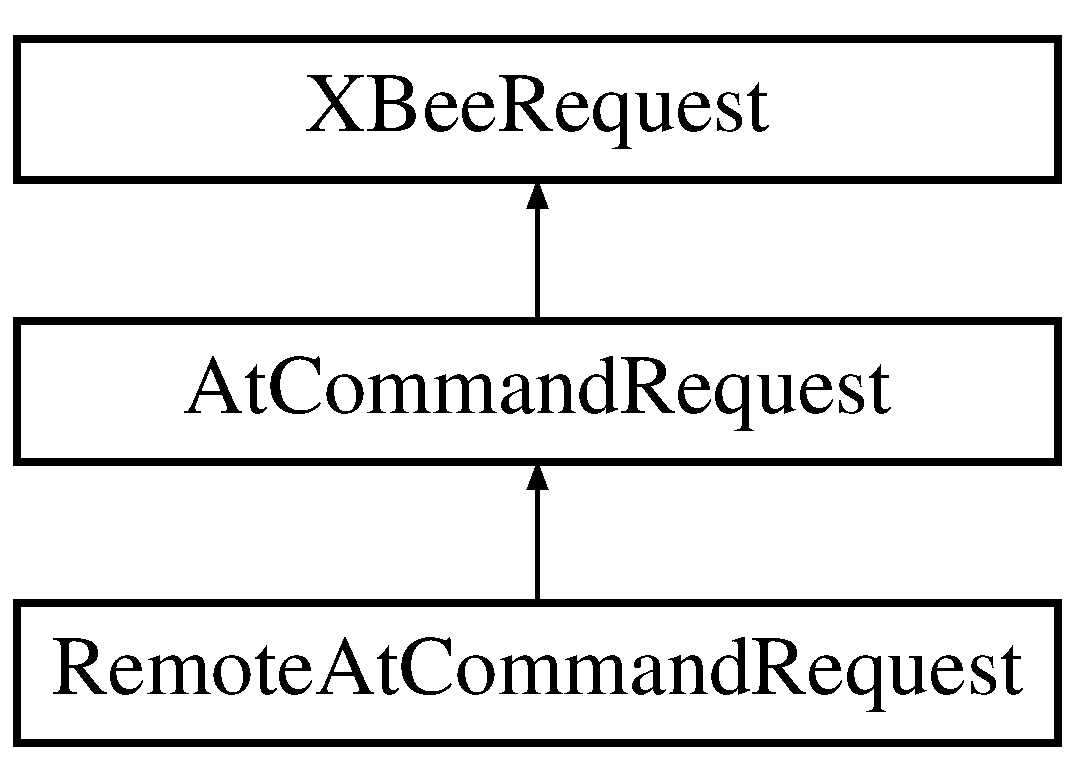
\includegraphics[height=3.000000cm]{classAtCommandRequest}
\end{center}
\end{figure}
\subsection*{\-Public \-Member \-Functions}
\begin{DoxyCompactItemize}
\item 
\hypertarget{classAtCommandRequest_ab62a1c4d5cd0d99cfb3e55fccd19f2fa}{{\bfseries \-At\-Command\-Request} (uint8\-\_\-t $\ast$command)}\label{classAtCommandRequest_ab62a1c4d5cd0d99cfb3e55fccd19f2fa}

\item 
\hypertarget{classAtCommandRequest_a20ca09437c349f4b71abbcb0bc007c56}{{\bfseries \-At\-Command\-Request} (uint8\-\_\-t $\ast$command, uint8\-\_\-t $\ast$command\-Value, uint8\-\_\-t command\-Value\-Length)}\label{classAtCommandRequest_a20ca09437c349f4b71abbcb0bc007c56}

\item 
uint8\-\_\-t \hyperlink{classAtCommandRequest_aa4fc8f0c8404172cd5532f3d8e5564f2}{get\-Frame\-Data} (uint8\-\_\-t pos)
\item 
uint8\-\_\-t \hyperlink{classAtCommandRequest_aad12b8357e63fca9e95b6731a4bfda0d}{get\-Frame\-Data\-Length} ()
\item 
\hypertarget{classAtCommandRequest_a5b2607da4f8f66fde9e87c25d575de7a}{uint8\-\_\-t $\ast$ {\bfseries get\-Command} ()}\label{classAtCommandRequest_a5b2607da4f8f66fde9e87c25d575de7a}

\item 
\hypertarget{classAtCommandRequest_aeae10ae23793aae47db036a0700407cc}{void {\bfseries set\-Command} (uint8\-\_\-t $\ast$command)}\label{classAtCommandRequest_aeae10ae23793aae47db036a0700407cc}

\item 
\hypertarget{classAtCommandRequest_a3faa9c8b83960d6464ab718a5f9179fa}{uint8\-\_\-t $\ast$ {\bfseries get\-Command\-Value} ()}\label{classAtCommandRequest_a3faa9c8b83960d6464ab718a5f9179fa}

\item 
\hypertarget{classAtCommandRequest_acd78ffba48b7c860c2be86f4a7787109}{void {\bfseries set\-Command\-Value} (uint8\-\_\-t $\ast$command)}\label{classAtCommandRequest_acd78ffba48b7c860c2be86f4a7787109}

\item 
\hypertarget{classAtCommandRequest_ac5a4595489d7c06779511243b38b99fb}{uint8\-\_\-t {\bfseries get\-Command\-Value\-Length} ()}\label{classAtCommandRequest_ac5a4595489d7c06779511243b38b99fb}

\item 
\hypertarget{classAtCommandRequest_a1fc2fb3033d4c7f1280c0989fd309519}{void {\bfseries set\-Command\-Value\-Length} (uint8\-\_\-t length)}\label{classAtCommandRequest_a1fc2fb3033d4c7f1280c0989fd309519}

\item 
void \hyperlink{classAtCommandRequest_a6842d0e270162c389d804eafd37a4f45}{clear\-Command\-Value} ()
\end{DoxyCompactItemize}


\subsection{\-Detailed \-Description}
\-Represents an \-A\-T \-Command \-T\-X packet \-The command is used to configure the serially connected \hyperlink{classXBee}{\-X\-Bee} radio 

\subsection{\-Member \-Function \-Documentation}
\hypertarget{classAtCommandRequest_a6842d0e270162c389d804eafd37a4f45}{\index{\-At\-Command\-Request@{\-At\-Command\-Request}!clear\-Command\-Value@{clear\-Command\-Value}}
\index{clear\-Command\-Value@{clear\-Command\-Value}!AtCommandRequest@{\-At\-Command\-Request}}
\subsubsection[{clear\-Command\-Value}]{\setlength{\rightskip}{0pt plus 5cm}void {\bf \-At\-Command\-Request\-::clear\-Command\-Value} (
\begin{DoxyParamCaption}
{}
\end{DoxyParamCaption}
)}}\label{classAtCommandRequest_a6842d0e270162c389d804eafd37a4f45}
\-Clears the optional command\-Value and command\-Value\-Length so that a query may be sent \hypertarget{classAtCommandRequest_aa4fc8f0c8404172cd5532f3d8e5564f2}{\index{\-At\-Command\-Request@{\-At\-Command\-Request}!get\-Frame\-Data@{get\-Frame\-Data}}
\index{get\-Frame\-Data@{get\-Frame\-Data}!AtCommandRequest@{\-At\-Command\-Request}}
\subsubsection[{get\-Frame\-Data}]{\setlength{\rightskip}{0pt plus 5cm}uint8\-\_\-t {\bf \-At\-Command\-Request\-::get\-Frame\-Data} (
\begin{DoxyParamCaption}
\item[{uint8\-\_\-t}]{pos}
\end{DoxyParamCaption}
)\hspace{0.3cm}{\ttfamily  \mbox{[}virtual\mbox{]}}}}\label{classAtCommandRequest_aa4fc8f0c8404172cd5532f3d8e5564f2}
\-Starting after the frame id (pos = 0) and up to but not including the checksum \-Note\-: \-Unlike \-Digi's definition of the frame data, this does not start with the \-A\-P\-I \-I\-D. \-The reason for this is the \-A\-P\-I \-I\-D and \-Frame \-I\-D are common to all requests, whereas my definition of frame data is only the \-A\-P\-I specific data. 

\-Implements \hyperlink{classXBeeRequest_ad5b998cd95a570bdaa4d74c6c8790d94}{\-X\-Bee\-Request}.



\-Reimplemented in \hyperlink{classRemoteAtCommandRequest_a0e576cf564ebd5a82cb2ed05239a856a}{\-Remote\-At\-Command\-Request}.

\hypertarget{classAtCommandRequest_aad12b8357e63fca9e95b6731a4bfda0d}{\index{\-At\-Command\-Request@{\-At\-Command\-Request}!get\-Frame\-Data\-Length@{get\-Frame\-Data\-Length}}
\index{get\-Frame\-Data\-Length@{get\-Frame\-Data\-Length}!AtCommandRequest@{\-At\-Command\-Request}}
\subsubsection[{get\-Frame\-Data\-Length}]{\setlength{\rightskip}{0pt plus 5cm}uint8\-\_\-t {\bf \-At\-Command\-Request\-::get\-Frame\-Data\-Length} (
\begin{DoxyParamCaption}
{}
\end{DoxyParamCaption}
)\hspace{0.3cm}{\ttfamily  \mbox{[}virtual\mbox{]}}}}\label{classAtCommandRequest_aad12b8357e63fca9e95b6731a4bfda0d}
\-Returns the size of the api frame (not including frame id or api id or checksum). 

\-Implements \hyperlink{classXBeeRequest_a03b6c558db5836fa7167c0fba7405642}{\-X\-Bee\-Request}.



\-Reimplemented in \hyperlink{classRemoteAtCommandRequest_a1d78334a8924b0a0e06de6ef3a09c24f}{\-Remote\-At\-Command\-Request}.



\-The documentation for this class was generated from the following files\-:\begin{DoxyCompactItemize}
\item 
\-X\-Bee.\-h\item 
\-X\-Bee.\-cpp\end{DoxyCompactItemize}

\hypertarget{classAtCommandResponse}{\section{\-At\-Command\-Response \-Class \-Reference}
\label{classAtCommandResponse}\index{\-At\-Command\-Response@{\-At\-Command\-Response}}
}


{\ttfamily \#include $<$\-X\-Bee.\-h$>$}

\-Inheritance diagram for \-At\-Command\-Response\-:\begin{figure}[H]
\begin{center}
\leavevmode
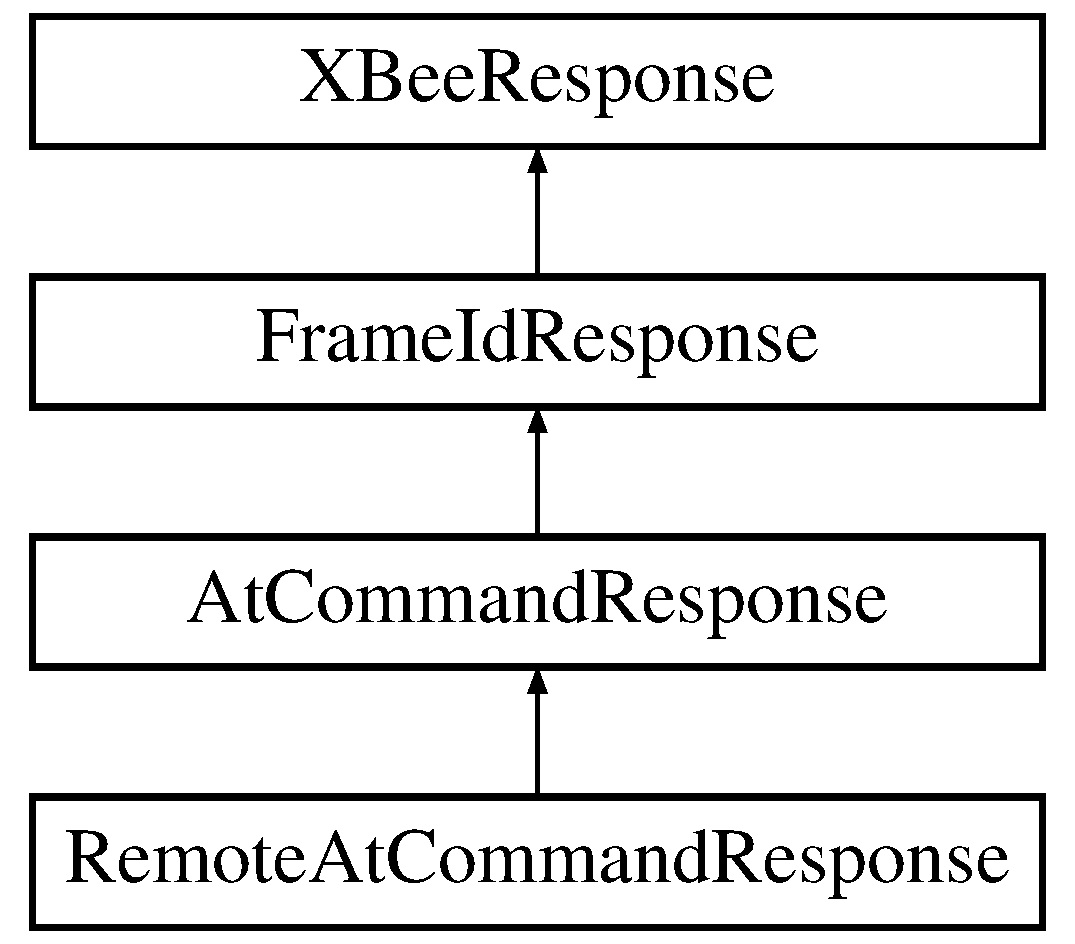
\includegraphics[height=4.000000cm]{classAtCommandResponse}
\end{center}
\end{figure}
\subsection*{\-Public \-Member \-Functions}
\begin{DoxyCompactItemize}
\item 
uint8\-\_\-t $\ast$ \hyperlink{classAtCommandResponse_a20f1bf08ba77f2bc74f009318a6fd133}{get\-Command} ()
\item 
uint8\-\_\-t \hyperlink{classAtCommandResponse_a340822cacf6eed3ef29955dc9610c09f}{get\-Status} ()
\item 
uint8\-\_\-t $\ast$ \hyperlink{classAtCommandResponse_ad1e2a0b6f8988536c570b116f103e7f9}{get\-Value} ()
\item 
uint8\-\_\-t \hyperlink{classAtCommandResponse_ad7d6159fa1777144e94a9ccfeaf83662}{get\-Value\-Length} ()
\item 
bool \hyperlink{classAtCommandResponse_ab606b3dc93f809b828b54e98a79711d8}{is\-Ok} ()
\end{DoxyCompactItemize}


\subsection{\-Detailed \-Description}
\-Represents an \-A\-T \-Command \-R\-X packet 

\subsection{\-Member \-Function \-Documentation}
\hypertarget{classAtCommandResponse_a20f1bf08ba77f2bc74f009318a6fd133}{\index{\-At\-Command\-Response@{\-At\-Command\-Response}!get\-Command@{get\-Command}}
\index{get\-Command@{get\-Command}!AtCommandResponse@{\-At\-Command\-Response}}
\subsubsection[{get\-Command}]{\setlength{\rightskip}{0pt plus 5cm}uint8\-\_\-t $\ast$ {\bf \-At\-Command\-Response\-::get\-Command} (
\begin{DoxyParamCaption}
{}
\end{DoxyParamCaption}
)}}\label{classAtCommandResponse_a20f1bf08ba77f2bc74f009318a6fd133}
\-Returns an array containing the two character command 

\-Reimplemented in \hyperlink{classRemoteAtCommandResponse_a6d26d626de8b8d0eaf8241b92ff39f28}{\-Remote\-At\-Command\-Response}.

\hypertarget{classAtCommandResponse_a340822cacf6eed3ef29955dc9610c09f}{\index{\-At\-Command\-Response@{\-At\-Command\-Response}!get\-Status@{get\-Status}}
\index{get\-Status@{get\-Status}!AtCommandResponse@{\-At\-Command\-Response}}
\subsubsection[{get\-Status}]{\setlength{\rightskip}{0pt plus 5cm}uint8\-\_\-t {\bf \-At\-Command\-Response\-::get\-Status} (
\begin{DoxyParamCaption}
{}
\end{DoxyParamCaption}
)}}\label{classAtCommandResponse_a340822cacf6eed3ef29955dc9610c09f}
\-Returns the command status code. \-Zero represents a successful command 

\-Reimplemented in \hyperlink{classRemoteAtCommandResponse_afc1b15612ea780c10dc1f33754868548}{\-Remote\-At\-Command\-Response}.

\hypertarget{classAtCommandResponse_ad1e2a0b6f8988536c570b116f103e7f9}{\index{\-At\-Command\-Response@{\-At\-Command\-Response}!get\-Value@{get\-Value}}
\index{get\-Value@{get\-Value}!AtCommandResponse@{\-At\-Command\-Response}}
\subsubsection[{get\-Value}]{\setlength{\rightskip}{0pt plus 5cm}uint8\-\_\-t $\ast$ {\bf \-At\-Command\-Response\-::get\-Value} (
\begin{DoxyParamCaption}
{}
\end{DoxyParamCaption}
)}}\label{classAtCommandResponse_ad1e2a0b6f8988536c570b116f103e7f9}
\-Returns an array containing the command value. \-This is only applicable to query commands. 

\-Reimplemented in \hyperlink{classRemoteAtCommandResponse_a3d72d768131c63271a62f75530efda29}{\-Remote\-At\-Command\-Response}.

\hypertarget{classAtCommandResponse_ad7d6159fa1777144e94a9ccfeaf83662}{\index{\-At\-Command\-Response@{\-At\-Command\-Response}!get\-Value\-Length@{get\-Value\-Length}}
\index{get\-Value\-Length@{get\-Value\-Length}!AtCommandResponse@{\-At\-Command\-Response}}
\subsubsection[{get\-Value\-Length}]{\setlength{\rightskip}{0pt plus 5cm}uint8\-\_\-t {\bf \-At\-Command\-Response\-::get\-Value\-Length} (
\begin{DoxyParamCaption}
{}
\end{DoxyParamCaption}
)}}\label{classAtCommandResponse_ad7d6159fa1777144e94a9ccfeaf83662}
\-Returns the length of the command value array. 

\-Reimplemented in \hyperlink{classRemoteAtCommandResponse_a55cf17381e461b8de4a2d5459bfc964a}{\-Remote\-At\-Command\-Response}.

\hypertarget{classAtCommandResponse_ab606b3dc93f809b828b54e98a79711d8}{\index{\-At\-Command\-Response@{\-At\-Command\-Response}!is\-Ok@{is\-Ok}}
\index{is\-Ok@{is\-Ok}!AtCommandResponse@{\-At\-Command\-Response}}
\subsubsection[{is\-Ok}]{\setlength{\rightskip}{0pt plus 5cm}bool {\bf \-At\-Command\-Response\-::is\-Ok} (
\begin{DoxyParamCaption}
{}
\end{DoxyParamCaption}
)}}\label{classAtCommandResponse_ab606b3dc93f809b828b54e98a79711d8}
\-Returns true if status equals \-A\-T\-\_\-\-O\-K 

\-Reimplemented in \hyperlink{classRemoteAtCommandResponse_a0cef7b3846d9c208ebd7ce4473aa90d3}{\-Remote\-At\-Command\-Response}.



\-The documentation for this class was generated from the following files\-:\begin{DoxyCompactItemize}
\item 
\-X\-Bee.\-h\item 
\-X\-Bee.\-cpp\end{DoxyCompactItemize}

\hypertarget{classFrameIdResponse}{\section{\-Frame\-Id\-Response \-Class \-Reference}
\label{classFrameIdResponse}\index{\-Frame\-Id\-Response@{\-Frame\-Id\-Response}}
}


{\ttfamily \#include $<$\-X\-Bee.\-h$>$}

\-Inheritance diagram for \-Frame\-Id\-Response\-:\begin{figure}[H]
\begin{center}
\leavevmode
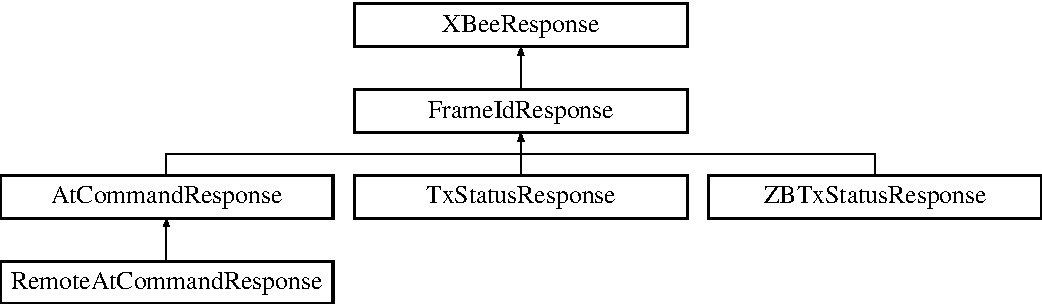
\includegraphics[height=4.000000cm]{classFrameIdResponse}
\end{center}
\end{figure}
\subsection*{\-Public \-Member \-Functions}
\begin{DoxyCompactItemize}
\item 
\hypertarget{classFrameIdResponse_a65a801fb25e995e3f1b048934b9cf803}{uint8\-\_\-t {\bfseries get\-Frame\-Id} ()}\label{classFrameIdResponse_a65a801fb25e995e3f1b048934b9cf803}

\end{DoxyCompactItemize}


\subsection{\-Detailed \-Description}
\-This class is extended by all \-Responses that include a frame id 

\-The documentation for this class was generated from the following files\-:\begin{DoxyCompactItemize}
\item 
\-X\-Bee.\-h\item 
\-X\-Bee.\-cpp\end{DoxyCompactItemize}

\hypertarget{classModemStatusResponse}{\section{\-Modem\-Status\-Response \-Class \-Reference}
\label{classModemStatusResponse}\index{\-Modem\-Status\-Response@{\-Modem\-Status\-Response}}
}


{\ttfamily \#include $<$\-X\-Bee.\-h$>$}

\-Inheritance diagram for \-Modem\-Status\-Response\-:\begin{figure}[H]
\begin{center}
\leavevmode
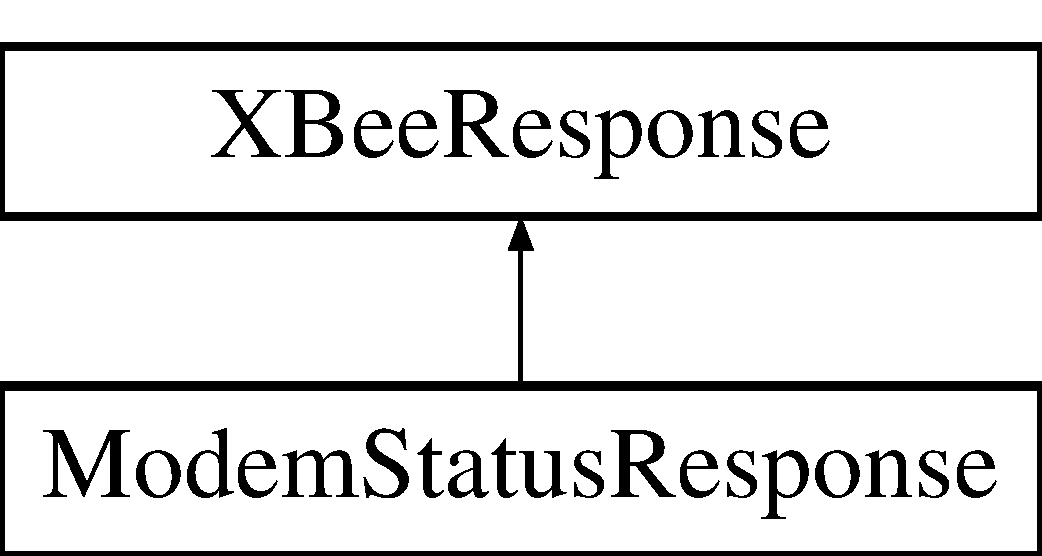
\includegraphics[height=2.000000cm]{classModemStatusResponse}
\end{center}
\end{figure}
\subsection*{\-Public \-Member \-Functions}
\begin{DoxyCompactItemize}
\item 
\hypertarget{classModemStatusResponse_a901244d6313391f60eec7764b10de3aa}{uint8\-\_\-t {\bfseries get\-Status} ()}\label{classModemStatusResponse_a901244d6313391f60eec7764b10de3aa}

\end{DoxyCompactItemize}


\subsection{\-Detailed \-Description}
\-Represents a \-Modem \-Status \-R\-X packet 

\-The documentation for this class was generated from the following files\-:\begin{DoxyCompactItemize}
\item 
\-X\-Bee.\-h\item 
\-X\-Bee.\-cpp\end{DoxyCompactItemize}

\hypertarget{classPayloadRequest}{\section{\-Payload\-Request \-Class \-Reference}
\label{classPayloadRequest}\index{\-Payload\-Request@{\-Payload\-Request}}
}


{\ttfamily \#include $<$\-X\-Bee.\-h$>$}

\-Inheritance diagram for \-Payload\-Request\-:\begin{figure}[H]
\begin{center}
\leavevmode
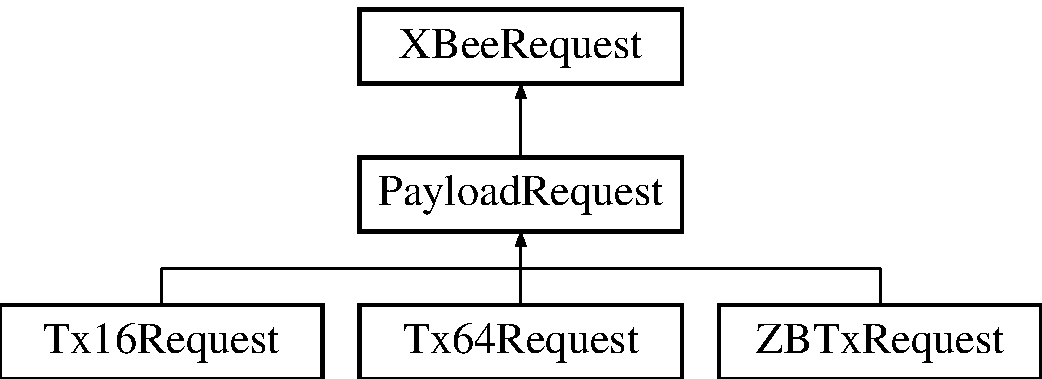
\includegraphics[height=3.000000cm]{classPayloadRequest}
\end{center}
\end{figure}
\subsection*{\-Public \-Member \-Functions}
\begin{DoxyCompactItemize}
\item 
\hypertarget{classPayloadRequest_a22cc9fd971a1334346560689d7d8c8d5}{{\bfseries \-Payload\-Request} (uint8\-\_\-t api\-Id, uint8\-\_\-t frame\-Id, uint8\-\_\-t $\ast$payload, uint8\-\_\-t payload\-Length)}\label{classPayloadRequest_a22cc9fd971a1334346560689d7d8c8d5}

\item 
uint8\-\_\-t $\ast$ \hyperlink{classPayloadRequest_a1e2d5757fefda70dfd0c567b3dd0ba39}{get\-Payload} ()
\item 
void \hyperlink{classPayloadRequest_aa9abc1f496a1c457f796207aa8a7567d}{set\-Payload} (uint8\-\_\-t $\ast$payload\-Ptr)
\item 
uint8\-\_\-t \hyperlink{classPayloadRequest_afb718d069f05611623833437c99893a4}{get\-Payload\-Length} ()
\item 
void \hyperlink{classPayloadRequest_a6e86a663ab6299afaa1cf21ad7c2c5c1}{set\-Payload\-Length} (uint8\-\_\-t payload\-Length)
\end{DoxyCompactItemize}


\subsection{\-Detailed \-Description}
\-All \-T\-X packets that support payloads extend this class 

\subsection{\-Member \-Function \-Documentation}
\hypertarget{classPayloadRequest_a1e2d5757fefda70dfd0c567b3dd0ba39}{\index{\-Payload\-Request@{\-Payload\-Request}!get\-Payload@{get\-Payload}}
\index{get\-Payload@{get\-Payload}!PayloadRequest@{\-Payload\-Request}}
\subsubsection[{get\-Payload}]{\setlength{\rightskip}{0pt plus 5cm}uint8\-\_\-t $\ast$ {\bf \-Payload\-Request\-::get\-Payload} (
\begin{DoxyParamCaption}
{}
\end{DoxyParamCaption}
)}}\label{classPayloadRequest_a1e2d5757fefda70dfd0c567b3dd0ba39}
\-Returns the payload of the packet, if not null \hypertarget{classPayloadRequest_afb718d069f05611623833437c99893a4}{\index{\-Payload\-Request@{\-Payload\-Request}!get\-Payload\-Length@{get\-Payload\-Length}}
\index{get\-Payload\-Length@{get\-Payload\-Length}!PayloadRequest@{\-Payload\-Request}}
\subsubsection[{get\-Payload\-Length}]{\setlength{\rightskip}{0pt plus 5cm}uint8\-\_\-t {\bf \-Payload\-Request\-::get\-Payload\-Length} (
\begin{DoxyParamCaption}
{}
\end{DoxyParamCaption}
)}}\label{classPayloadRequest_afb718d069f05611623833437c99893a4}
\-Returns the length of the payload array, as specified by the user. \hypertarget{classPayloadRequest_aa9abc1f496a1c457f796207aa8a7567d}{\index{\-Payload\-Request@{\-Payload\-Request}!set\-Payload@{set\-Payload}}
\index{set\-Payload@{set\-Payload}!PayloadRequest@{\-Payload\-Request}}
\subsubsection[{set\-Payload}]{\setlength{\rightskip}{0pt plus 5cm}void {\bf \-Payload\-Request\-::set\-Payload} (
\begin{DoxyParamCaption}
\item[{uint8\-\_\-t $\ast$}]{payload\-Ptr}
\end{DoxyParamCaption}
)}}\label{classPayloadRequest_aa9abc1f496a1c457f796207aa8a7567d}
\-Sets the payload array \hypertarget{classPayloadRequest_a6e86a663ab6299afaa1cf21ad7c2c5c1}{\index{\-Payload\-Request@{\-Payload\-Request}!set\-Payload\-Length@{set\-Payload\-Length}}
\index{set\-Payload\-Length@{set\-Payload\-Length}!PayloadRequest@{\-Payload\-Request}}
\subsubsection[{set\-Payload\-Length}]{\setlength{\rightskip}{0pt plus 5cm}void {\bf \-Payload\-Request\-::set\-Payload\-Length} (
\begin{DoxyParamCaption}
\item[{uint8\-\_\-t}]{payload\-Length}
\end{DoxyParamCaption}
)}}\label{classPayloadRequest_a6e86a663ab6299afaa1cf21ad7c2c5c1}
\-Sets the length of the payload to include in the request. \-For example if the payload array is 50 bytes and you only want the first 10 to be included in the packet, set the length to 10. \-Length must be $<$= to the array length. 

\-The documentation for this class was generated from the following files\-:\begin{DoxyCompactItemize}
\item 
\-X\-Bee.\-h\item 
\-X\-Bee.\-cpp\end{DoxyCompactItemize}

\hypertarget{classRemoteAtCommandRequest}{\section{\-Remote\-At\-Command\-Request \-Class \-Reference}
\label{classRemoteAtCommandRequest}\index{\-Remote\-At\-Command\-Request@{\-Remote\-At\-Command\-Request}}
}


{\ttfamily \#include $<$\-X\-Bee.\-h$>$}

\-Inheritance diagram for \-Remote\-At\-Command\-Request\-:\begin{figure}[H]
\begin{center}
\leavevmode
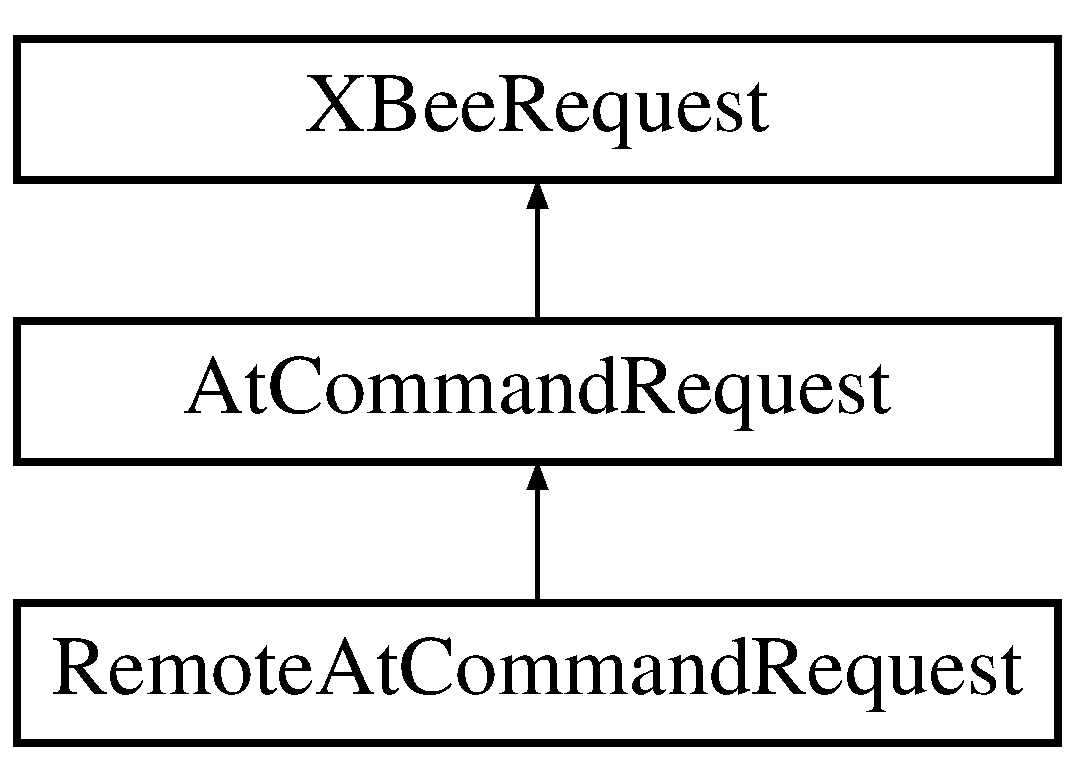
\includegraphics[height=3.000000cm]{classRemoteAtCommandRequest}
\end{center}
\end{figure}
\subsection*{\-Public \-Member \-Functions}
\begin{DoxyCompactItemize}
\item 
\hyperlink{classRemoteAtCommandRequest_ac6977fe584bab7d7414b0c45d1ae37cc}{\-Remote\-At\-Command\-Request} (uint16\-\_\-t remote\-Address16, uint8\-\_\-t $\ast$command, uint8\-\_\-t $\ast$command\-Value, uint8\-\_\-t command\-Value\-Length)
\item 
\hyperlink{classRemoteAtCommandRequest_ae8139e39010dcd8956a4281109885a81}{\-Remote\-At\-Command\-Request} (uint16\-\_\-t remote\-Address16, uint8\-\_\-t $\ast$command)
\item 
\hyperlink{classRemoteAtCommandRequest_ae49de42cdec0b9689882e2372a3bae1d}{\-Remote\-At\-Command\-Request} (\hyperlink{classXBeeAddress64}{\-X\-Bee\-Address64} \&remote\-Address64, uint8\-\_\-t $\ast$command, uint8\-\_\-t $\ast$command\-Value, uint8\-\_\-t command\-Value\-Length)
\item 
\hyperlink{classRemoteAtCommandRequest_aa01b3f59d62d444ad78d6f1bbf8124aa}{\-Remote\-At\-Command\-Request} (\hyperlink{classXBeeAddress64}{\-X\-Bee\-Address64} \&remote\-Address64, uint8\-\_\-t $\ast$command)
\item 
\hypertarget{classRemoteAtCommandRequest_a1802fa7c5d644184f19fcd3da839f08a}{uint16\-\_\-t {\bfseries get\-Remote\-Address16} ()}\label{classRemoteAtCommandRequest_a1802fa7c5d644184f19fcd3da839f08a}

\item 
\hypertarget{classRemoteAtCommandRequest_a91d4ee0fa25a634e419df1b0059f6073}{void {\bfseries set\-Remote\-Address16} (uint16\-\_\-t remote\-Address16)}\label{classRemoteAtCommandRequest_a91d4ee0fa25a634e419df1b0059f6073}

\item 
\hypertarget{classRemoteAtCommandRequest_ab6c602ded638f7740ac69319915e0389}{\hyperlink{classXBeeAddress64}{\-X\-Bee\-Address64} \& {\bfseries get\-Remote\-Address64} ()}\label{classRemoteAtCommandRequest_ab6c602ded638f7740ac69319915e0389}

\item 
\hypertarget{classRemoteAtCommandRequest_abf42b8f760f1f1959de090f4493e928b}{void {\bfseries set\-Remote\-Address64} (\hyperlink{classXBeeAddress64}{\-X\-Bee\-Address64} \&remote\-Address64)}\label{classRemoteAtCommandRequest_abf42b8f760f1f1959de090f4493e928b}

\item 
\hypertarget{classRemoteAtCommandRequest_ad9098bc0358fa44f73c0cc51bc244bf3}{bool {\bfseries get\-Apply\-Changes} ()}\label{classRemoteAtCommandRequest_ad9098bc0358fa44f73c0cc51bc244bf3}

\item 
\hypertarget{classRemoteAtCommandRequest_aab7cf2bf1ca644a17bede9abd3929acd}{void {\bfseries set\-Apply\-Changes} (bool apply\-Changes)}\label{classRemoteAtCommandRequest_aab7cf2bf1ca644a17bede9abd3929acd}

\item 
uint8\-\_\-t \hyperlink{classRemoteAtCommandRequest_a0e576cf564ebd5a82cb2ed05239a856a}{get\-Frame\-Data} (uint8\-\_\-t pos)
\item 
uint8\-\_\-t \hyperlink{classRemoteAtCommandRequest_a1d78334a8924b0a0e06de6ef3a09c24f}{get\-Frame\-Data\-Length} ()
\end{DoxyCompactItemize}
\subsection*{\-Static \-Public \-Attributes}
\begin{DoxyCompactItemize}
\item 
\hypertarget{classRemoteAtCommandRequest_a72668f0e22df605d5b32141bd7ca0256}{static \hyperlink{classXBeeAddress64}{\-X\-Bee\-Address64} {\bfseries broadcast\-Address64} = \hyperlink{classXBeeAddress64}{\-X\-Bee\-Address64}(0x0, B\-R\-O\-A\-D\-C\-A\-S\-T\-\_\-\-A\-D\-D\-R\-E\-S\-S)}\label{classRemoteAtCommandRequest_a72668f0e22df605d5b32141bd7ca0256}

\end{DoxyCompactItemize}


\subsection{\-Detailed \-Description}
\-Represents an \-Remote \-A\-T \-Command \-T\-X packet \-The command is used to configure a remote \hyperlink{classXBee}{\-X\-Bee} radio 

\subsection{\-Constructor \& \-Destructor \-Documentation}
\hypertarget{classRemoteAtCommandRequest_ac6977fe584bab7d7414b0c45d1ae37cc}{\index{\-Remote\-At\-Command\-Request@{\-Remote\-At\-Command\-Request}!\-Remote\-At\-Command\-Request@{\-Remote\-At\-Command\-Request}}
\index{\-Remote\-At\-Command\-Request@{\-Remote\-At\-Command\-Request}!RemoteAtCommandRequest@{\-Remote\-At\-Command\-Request}}
\subsubsection[{\-Remote\-At\-Command\-Request}]{\setlength{\rightskip}{0pt plus 5cm}\-Remote\-At\-Command\-Request\-::\-Remote\-At\-Command\-Request (
\begin{DoxyParamCaption}
\item[{uint16\-\_\-t}]{remote\-Address16, }
\item[{uint8\-\_\-t $\ast$}]{command, }
\item[{uint8\-\_\-t $\ast$}]{command\-Value, }
\item[{uint8\-\_\-t}]{command\-Value\-Length}
\end{DoxyParamCaption}
)}}\label{classRemoteAtCommandRequest_ac6977fe584bab7d7414b0c45d1ae37cc}
\-Creates a \hyperlink{classRemoteAtCommandRequest}{\-Remote\-At\-Command\-Request} with 16-\/bit address to set a command. 64-\/bit address defaults to broadcast and apply\-Changes is true. \hypertarget{classRemoteAtCommandRequest_ae8139e39010dcd8956a4281109885a81}{\index{\-Remote\-At\-Command\-Request@{\-Remote\-At\-Command\-Request}!\-Remote\-At\-Command\-Request@{\-Remote\-At\-Command\-Request}}
\index{\-Remote\-At\-Command\-Request@{\-Remote\-At\-Command\-Request}!RemoteAtCommandRequest@{\-Remote\-At\-Command\-Request}}
\subsubsection[{\-Remote\-At\-Command\-Request}]{\setlength{\rightskip}{0pt plus 5cm}\-Remote\-At\-Command\-Request\-::\-Remote\-At\-Command\-Request (
\begin{DoxyParamCaption}
\item[{uint16\-\_\-t}]{remote\-Address16, }
\item[{uint8\-\_\-t $\ast$}]{command}
\end{DoxyParamCaption}
)}}\label{classRemoteAtCommandRequest_ae8139e39010dcd8956a4281109885a81}
\-Creates a \hyperlink{classRemoteAtCommandRequest}{\-Remote\-At\-Command\-Request} with 16-\/bit address to query a command. 64-\/bit address defaults to broadcast and apply\-Changes is true. \hypertarget{classRemoteAtCommandRequest_ae49de42cdec0b9689882e2372a3bae1d}{\index{\-Remote\-At\-Command\-Request@{\-Remote\-At\-Command\-Request}!\-Remote\-At\-Command\-Request@{\-Remote\-At\-Command\-Request}}
\index{\-Remote\-At\-Command\-Request@{\-Remote\-At\-Command\-Request}!RemoteAtCommandRequest@{\-Remote\-At\-Command\-Request}}
\subsubsection[{\-Remote\-At\-Command\-Request}]{\setlength{\rightskip}{0pt plus 5cm}\-Remote\-At\-Command\-Request\-::\-Remote\-At\-Command\-Request (
\begin{DoxyParamCaption}
\item[{{\bf \-X\-Bee\-Address64} \&}]{remote\-Address64, }
\item[{uint8\-\_\-t $\ast$}]{command, }
\item[{uint8\-\_\-t $\ast$}]{command\-Value, }
\item[{uint8\-\_\-t}]{command\-Value\-Length}
\end{DoxyParamCaption}
)}}\label{classRemoteAtCommandRequest_ae49de42cdec0b9689882e2372a3bae1d}
\-Creates a \hyperlink{classRemoteAtCommandRequest}{\-Remote\-At\-Command\-Request} with 64-\/bit address to set a command. 16-\/bit address defaults to broadcast and apply\-Changes is true. \hypertarget{classRemoteAtCommandRequest_aa01b3f59d62d444ad78d6f1bbf8124aa}{\index{\-Remote\-At\-Command\-Request@{\-Remote\-At\-Command\-Request}!\-Remote\-At\-Command\-Request@{\-Remote\-At\-Command\-Request}}
\index{\-Remote\-At\-Command\-Request@{\-Remote\-At\-Command\-Request}!RemoteAtCommandRequest@{\-Remote\-At\-Command\-Request}}
\subsubsection[{\-Remote\-At\-Command\-Request}]{\setlength{\rightskip}{0pt plus 5cm}\-Remote\-At\-Command\-Request\-::\-Remote\-At\-Command\-Request (
\begin{DoxyParamCaption}
\item[{{\bf \-X\-Bee\-Address64} \&}]{remote\-Address64, }
\item[{uint8\-\_\-t $\ast$}]{command}
\end{DoxyParamCaption}
)}}\label{classRemoteAtCommandRequest_aa01b3f59d62d444ad78d6f1bbf8124aa}
\-Creates a \hyperlink{classRemoteAtCommandRequest}{\-Remote\-At\-Command\-Request} with 16-\/bit address to query a command. 16-\/bit address defaults to broadcast and apply\-Changes is true. 

\subsection{\-Member \-Function \-Documentation}
\hypertarget{classRemoteAtCommandRequest_a0e576cf564ebd5a82cb2ed05239a856a}{\index{\-Remote\-At\-Command\-Request@{\-Remote\-At\-Command\-Request}!get\-Frame\-Data@{get\-Frame\-Data}}
\index{get\-Frame\-Data@{get\-Frame\-Data}!RemoteAtCommandRequest@{\-Remote\-At\-Command\-Request}}
\subsubsection[{get\-Frame\-Data}]{\setlength{\rightskip}{0pt plus 5cm}uint8\-\_\-t {\bf \-Remote\-At\-Command\-Request\-::get\-Frame\-Data} (
\begin{DoxyParamCaption}
\item[{uint8\-\_\-t}]{pos}
\end{DoxyParamCaption}
)\hspace{0.3cm}{\ttfamily  \mbox{[}virtual\mbox{]}}}}\label{classRemoteAtCommandRequest_a0e576cf564ebd5a82cb2ed05239a856a}
\-Starting after the frame id (pos = 0) and up to but not including the checksum \-Note\-: \-Unlike \-Digi's definition of the frame data, this does not start with the \-A\-P\-I \-I\-D. \-The reason for this is the \-A\-P\-I \-I\-D and \-Frame \-I\-D are common to all requests, whereas my definition of frame data is only the \-A\-P\-I specific data. 

\-Reimplemented from \hyperlink{classAtCommandRequest_aa4fc8f0c8404172cd5532f3d8e5564f2}{\-At\-Command\-Request}.

\hypertarget{classRemoteAtCommandRequest_a1d78334a8924b0a0e06de6ef3a09c24f}{\index{\-Remote\-At\-Command\-Request@{\-Remote\-At\-Command\-Request}!get\-Frame\-Data\-Length@{get\-Frame\-Data\-Length}}
\index{get\-Frame\-Data\-Length@{get\-Frame\-Data\-Length}!RemoteAtCommandRequest@{\-Remote\-At\-Command\-Request}}
\subsubsection[{get\-Frame\-Data\-Length}]{\setlength{\rightskip}{0pt plus 5cm}uint8\-\_\-t {\bf \-Remote\-At\-Command\-Request\-::get\-Frame\-Data\-Length} (
\begin{DoxyParamCaption}
{}
\end{DoxyParamCaption}
)\hspace{0.3cm}{\ttfamily  \mbox{[}virtual\mbox{]}}}}\label{classRemoteAtCommandRequest_a1d78334a8924b0a0e06de6ef3a09c24f}
\-Returns the size of the api frame (not including frame id or api id or checksum). 

\-Reimplemented from \hyperlink{classAtCommandRequest_aad12b8357e63fca9e95b6731a4bfda0d}{\-At\-Command\-Request}.



\-The documentation for this class was generated from the following files\-:\begin{DoxyCompactItemize}
\item 
\-X\-Bee.\-h\item 
\-X\-Bee.\-cpp\end{DoxyCompactItemize}

\hypertarget{classRemoteAtCommandResponse}{\section{\-Remote\-At\-Command\-Response \-Class \-Reference}
\label{classRemoteAtCommandResponse}\index{\-Remote\-At\-Command\-Response@{\-Remote\-At\-Command\-Response}}
}


{\ttfamily \#include $<$\-X\-Bee.\-h$>$}

\-Inheritance diagram for \-Remote\-At\-Command\-Response\-:\begin{figure}[H]
\begin{center}
\leavevmode
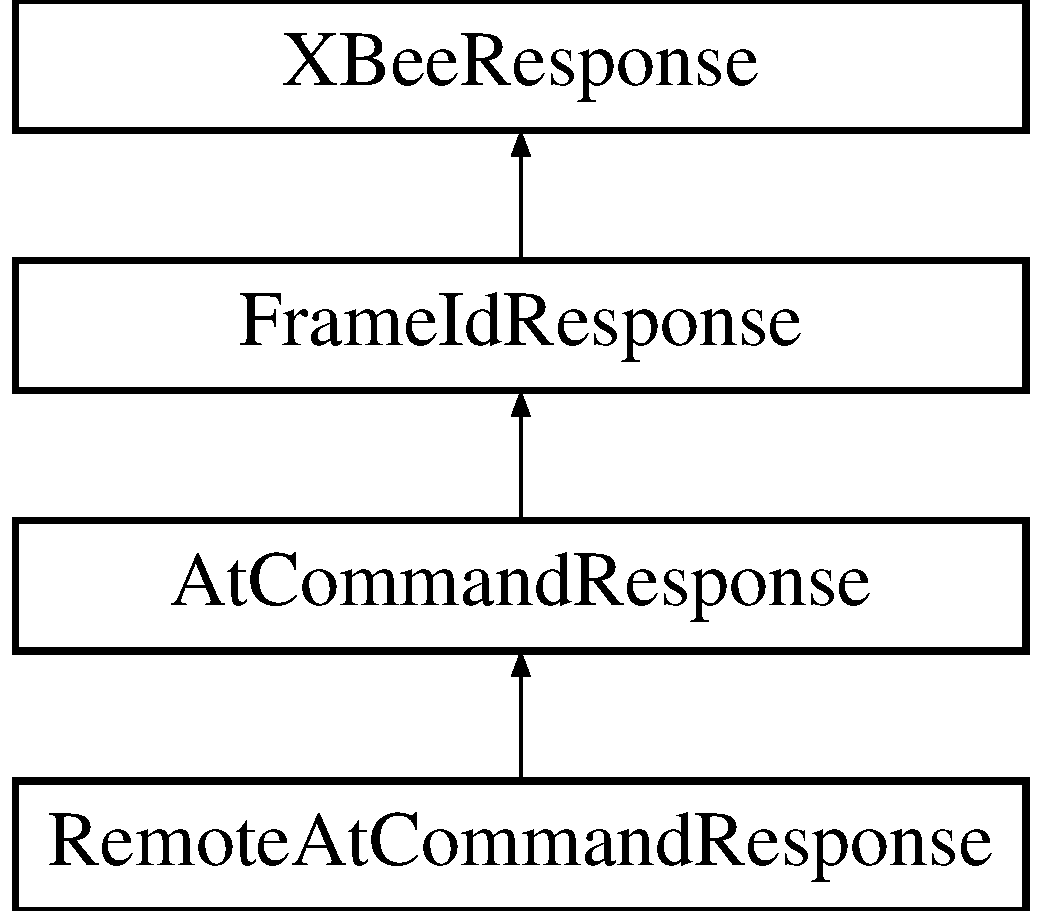
\includegraphics[height=4.000000cm]{classRemoteAtCommandResponse}
\end{center}
\end{figure}
\subsection*{\-Public \-Member \-Functions}
\begin{DoxyCompactItemize}
\item 
uint8\-\_\-t $\ast$ \hyperlink{classRemoteAtCommandResponse_a6d26d626de8b8d0eaf8241b92ff39f28}{get\-Command} ()
\item 
uint8\-\_\-t \hyperlink{classRemoteAtCommandResponse_afc1b15612ea780c10dc1f33754868548}{get\-Status} ()
\item 
uint8\-\_\-t $\ast$ \hyperlink{classRemoteAtCommandResponse_a3d72d768131c63271a62f75530efda29}{get\-Value} ()
\item 
uint8\-\_\-t \hyperlink{classRemoteAtCommandResponse_a55cf17381e461b8de4a2d5459bfc964a}{get\-Value\-Length} ()
\item 
uint16\-\_\-t \hyperlink{classRemoteAtCommandResponse_a2bea13bca12330a2eb1da3e3f0224bde}{get\-Remote\-Address16} ()
\item 
\hyperlink{classXBeeAddress64}{\-X\-Bee\-Address64} \& \hyperlink{classRemoteAtCommandResponse_ab87802214e04a7058ed0dc9668e70e73}{get\-Remote\-Address64} ()
\item 
bool \hyperlink{classRemoteAtCommandResponse_a0cef7b3846d9c208ebd7ce4473aa90d3}{is\-Ok} ()
\end{DoxyCompactItemize}


\subsection{\-Detailed \-Description}
\-Represents a \-Remote \-A\-T \-Command \-R\-X packet 

\subsection{\-Member \-Function \-Documentation}
\hypertarget{classRemoteAtCommandResponse_a6d26d626de8b8d0eaf8241b92ff39f28}{\index{\-Remote\-At\-Command\-Response@{\-Remote\-At\-Command\-Response}!get\-Command@{get\-Command}}
\index{get\-Command@{get\-Command}!RemoteAtCommandResponse@{\-Remote\-At\-Command\-Response}}
\subsubsection[{get\-Command}]{\setlength{\rightskip}{0pt plus 5cm}uint8\-\_\-t $\ast$ {\bf \-Remote\-At\-Command\-Response\-::get\-Command} (
\begin{DoxyParamCaption}
{}
\end{DoxyParamCaption}
)}}\label{classRemoteAtCommandResponse_a6d26d626de8b8d0eaf8241b92ff39f28}
\-Returns an array containing the two character command 

\-Reimplemented from \hyperlink{classAtCommandResponse_a20f1bf08ba77f2bc74f009318a6fd133}{\-At\-Command\-Response}.

\hypertarget{classRemoteAtCommandResponse_a2bea13bca12330a2eb1da3e3f0224bde}{\index{\-Remote\-At\-Command\-Response@{\-Remote\-At\-Command\-Response}!get\-Remote\-Address16@{get\-Remote\-Address16}}
\index{get\-Remote\-Address16@{get\-Remote\-Address16}!RemoteAtCommandResponse@{\-Remote\-At\-Command\-Response}}
\subsubsection[{get\-Remote\-Address16}]{\setlength{\rightskip}{0pt plus 5cm}uint16\-\_\-t {\bf \-Remote\-At\-Command\-Response\-::get\-Remote\-Address16} (
\begin{DoxyParamCaption}
{}
\end{DoxyParamCaption}
)}}\label{classRemoteAtCommandResponse_a2bea13bca12330a2eb1da3e3f0224bde}
\-Returns the 16-\/bit address of the remote radio \hypertarget{classRemoteAtCommandResponse_ab87802214e04a7058ed0dc9668e70e73}{\index{\-Remote\-At\-Command\-Response@{\-Remote\-At\-Command\-Response}!get\-Remote\-Address64@{get\-Remote\-Address64}}
\index{get\-Remote\-Address64@{get\-Remote\-Address64}!RemoteAtCommandResponse@{\-Remote\-At\-Command\-Response}}
\subsubsection[{get\-Remote\-Address64}]{\setlength{\rightskip}{0pt plus 5cm}{\bf \-X\-Bee\-Address64} \& {\bf \-Remote\-At\-Command\-Response\-::get\-Remote\-Address64} (
\begin{DoxyParamCaption}
{}
\end{DoxyParamCaption}
)}}\label{classRemoteAtCommandResponse_ab87802214e04a7058ed0dc9668e70e73}
\-Returns the 64-\/bit address of the remote radio \hypertarget{classRemoteAtCommandResponse_afc1b15612ea780c10dc1f33754868548}{\index{\-Remote\-At\-Command\-Response@{\-Remote\-At\-Command\-Response}!get\-Status@{get\-Status}}
\index{get\-Status@{get\-Status}!RemoteAtCommandResponse@{\-Remote\-At\-Command\-Response}}
\subsubsection[{get\-Status}]{\setlength{\rightskip}{0pt plus 5cm}uint8\-\_\-t {\bf \-Remote\-At\-Command\-Response\-::get\-Status} (
\begin{DoxyParamCaption}
{}
\end{DoxyParamCaption}
)}}\label{classRemoteAtCommandResponse_afc1b15612ea780c10dc1f33754868548}
\-Returns the command status code. \-Zero represents a successful command 

\-Reimplemented from \hyperlink{classAtCommandResponse_a340822cacf6eed3ef29955dc9610c09f}{\-At\-Command\-Response}.

\hypertarget{classRemoteAtCommandResponse_a3d72d768131c63271a62f75530efda29}{\index{\-Remote\-At\-Command\-Response@{\-Remote\-At\-Command\-Response}!get\-Value@{get\-Value}}
\index{get\-Value@{get\-Value}!RemoteAtCommandResponse@{\-Remote\-At\-Command\-Response}}
\subsubsection[{get\-Value}]{\setlength{\rightskip}{0pt plus 5cm}uint8\-\_\-t $\ast$ {\bf \-Remote\-At\-Command\-Response\-::get\-Value} (
\begin{DoxyParamCaption}
{}
\end{DoxyParamCaption}
)}}\label{classRemoteAtCommandResponse_a3d72d768131c63271a62f75530efda29}
\-Returns an array containing the command value. \-This is only applicable to query commands. 

\-Reimplemented from \hyperlink{classAtCommandResponse_ad1e2a0b6f8988536c570b116f103e7f9}{\-At\-Command\-Response}.

\hypertarget{classRemoteAtCommandResponse_a55cf17381e461b8de4a2d5459bfc964a}{\index{\-Remote\-At\-Command\-Response@{\-Remote\-At\-Command\-Response}!get\-Value\-Length@{get\-Value\-Length}}
\index{get\-Value\-Length@{get\-Value\-Length}!RemoteAtCommandResponse@{\-Remote\-At\-Command\-Response}}
\subsubsection[{get\-Value\-Length}]{\setlength{\rightskip}{0pt plus 5cm}uint8\-\_\-t {\bf \-Remote\-At\-Command\-Response\-::get\-Value\-Length} (
\begin{DoxyParamCaption}
{}
\end{DoxyParamCaption}
)}}\label{classRemoteAtCommandResponse_a55cf17381e461b8de4a2d5459bfc964a}
\-Returns the length of the command value array. 

\-Reimplemented from \hyperlink{classAtCommandResponse_ad7d6159fa1777144e94a9ccfeaf83662}{\-At\-Command\-Response}.

\hypertarget{classRemoteAtCommandResponse_a0cef7b3846d9c208ebd7ce4473aa90d3}{\index{\-Remote\-At\-Command\-Response@{\-Remote\-At\-Command\-Response}!is\-Ok@{is\-Ok}}
\index{is\-Ok@{is\-Ok}!RemoteAtCommandResponse@{\-Remote\-At\-Command\-Response}}
\subsubsection[{is\-Ok}]{\setlength{\rightskip}{0pt plus 5cm}bool {\bf \-Remote\-At\-Command\-Response\-::is\-Ok} (
\begin{DoxyParamCaption}
{}
\end{DoxyParamCaption}
)}}\label{classRemoteAtCommandResponse_a0cef7b3846d9c208ebd7ce4473aa90d3}
\-Returns true if command was successful 

\-Reimplemented from \hyperlink{classAtCommandResponse_ab606b3dc93f809b828b54e98a79711d8}{\-At\-Command\-Response}.



\-The documentation for this class was generated from the following files\-:\begin{DoxyCompactItemize}
\item 
\-X\-Bee.\-h\item 
\-X\-Bee.\-cpp\end{DoxyCompactItemize}

\hypertarget{classRx16IoSampleResponse}{\section{\-Rx16\-Io\-Sample\-Response \-Class \-Reference}
\label{classRx16IoSampleResponse}\index{\-Rx16\-Io\-Sample\-Response@{\-Rx16\-Io\-Sample\-Response}}
}
\-Inheritance diagram for \-Rx16\-Io\-Sample\-Response\-:\begin{figure}[H]
\begin{center}
\leavevmode
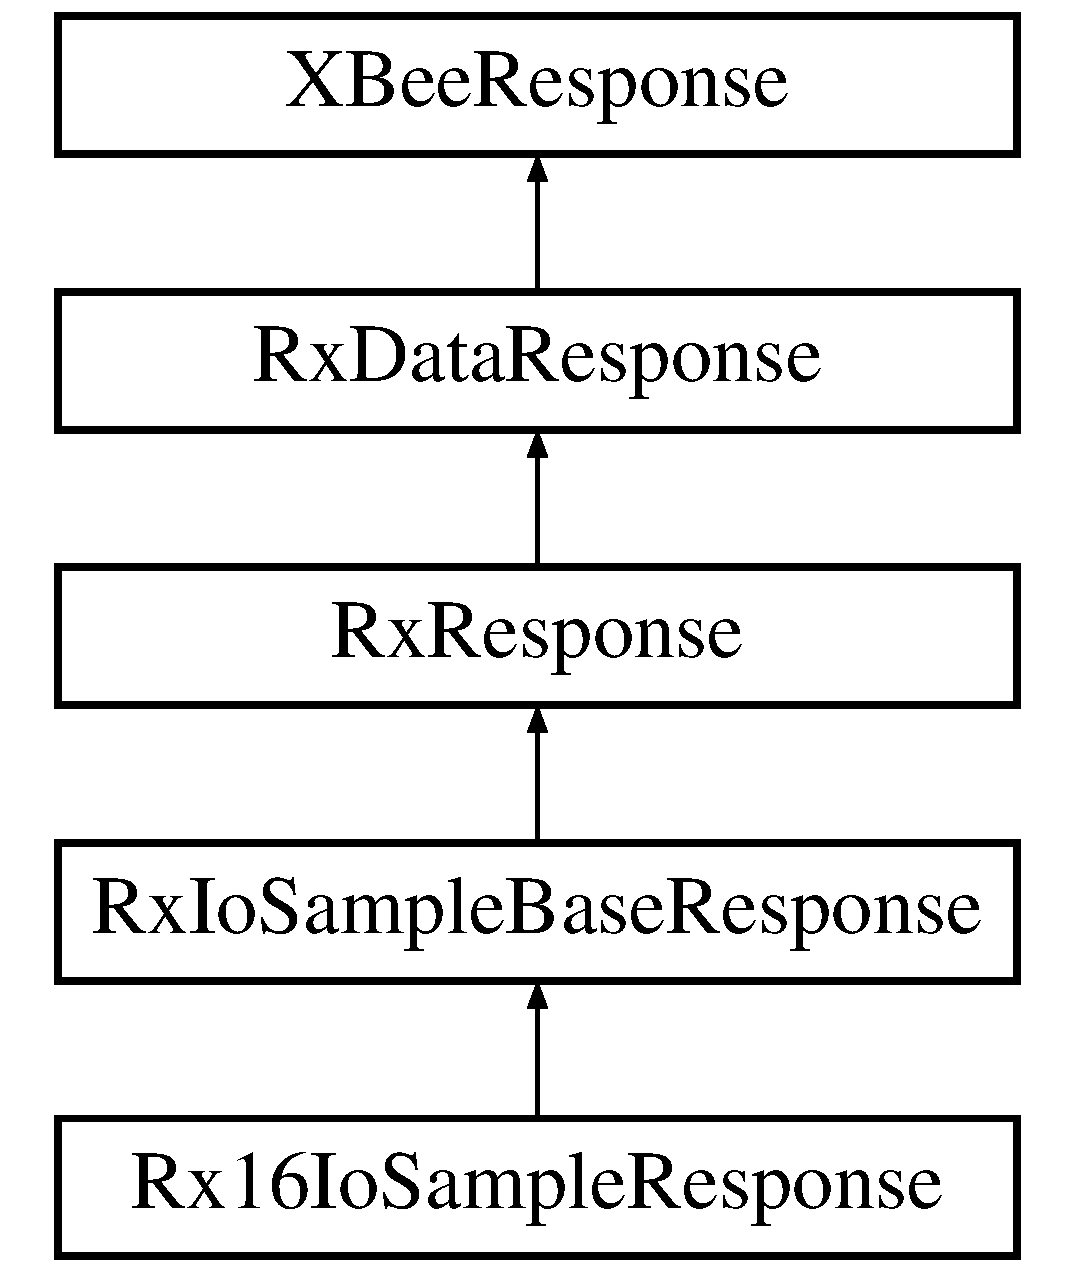
\includegraphics[height=5.000000cm]{classRx16IoSampleResponse}
\end{center}
\end{figure}
\subsection*{\-Public \-Member \-Functions}
\begin{DoxyCompactItemize}
\item 
\hypertarget{classRx16IoSampleResponse_ab35f8039eebc6c969563f769fdae8f21}{uint16\-\_\-t {\bfseries get\-Remote\-Address16} ()}\label{classRx16IoSampleResponse_ab35f8039eebc6c969563f769fdae8f21}

\item 
\hypertarget{classRx16IoSampleResponse_a3b3437d05701cdaf86bc54a5a2acb026}{uint8\-\_\-t {\bfseries get\-Rssi\-Offset} ()}\label{classRx16IoSampleResponse_a3b3437d05701cdaf86bc54a5a2acb026}

\end{DoxyCompactItemize}


\-The documentation for this class was generated from the following files\-:\begin{DoxyCompactItemize}
\item 
\-X\-Bee.\-h\item 
\-X\-Bee.\-cpp\end{DoxyCompactItemize}

\hypertarget{classRx16Response}{\section{\-Rx16\-Response \-Class \-Reference}
\label{classRx16Response}\index{\-Rx16\-Response@{\-Rx16\-Response}}
}


{\ttfamily \#include $<$\-X\-Bee.\-h$>$}

\-Inheritance diagram for \-Rx16\-Response\-:\begin{figure}[H]
\begin{center}
\leavevmode
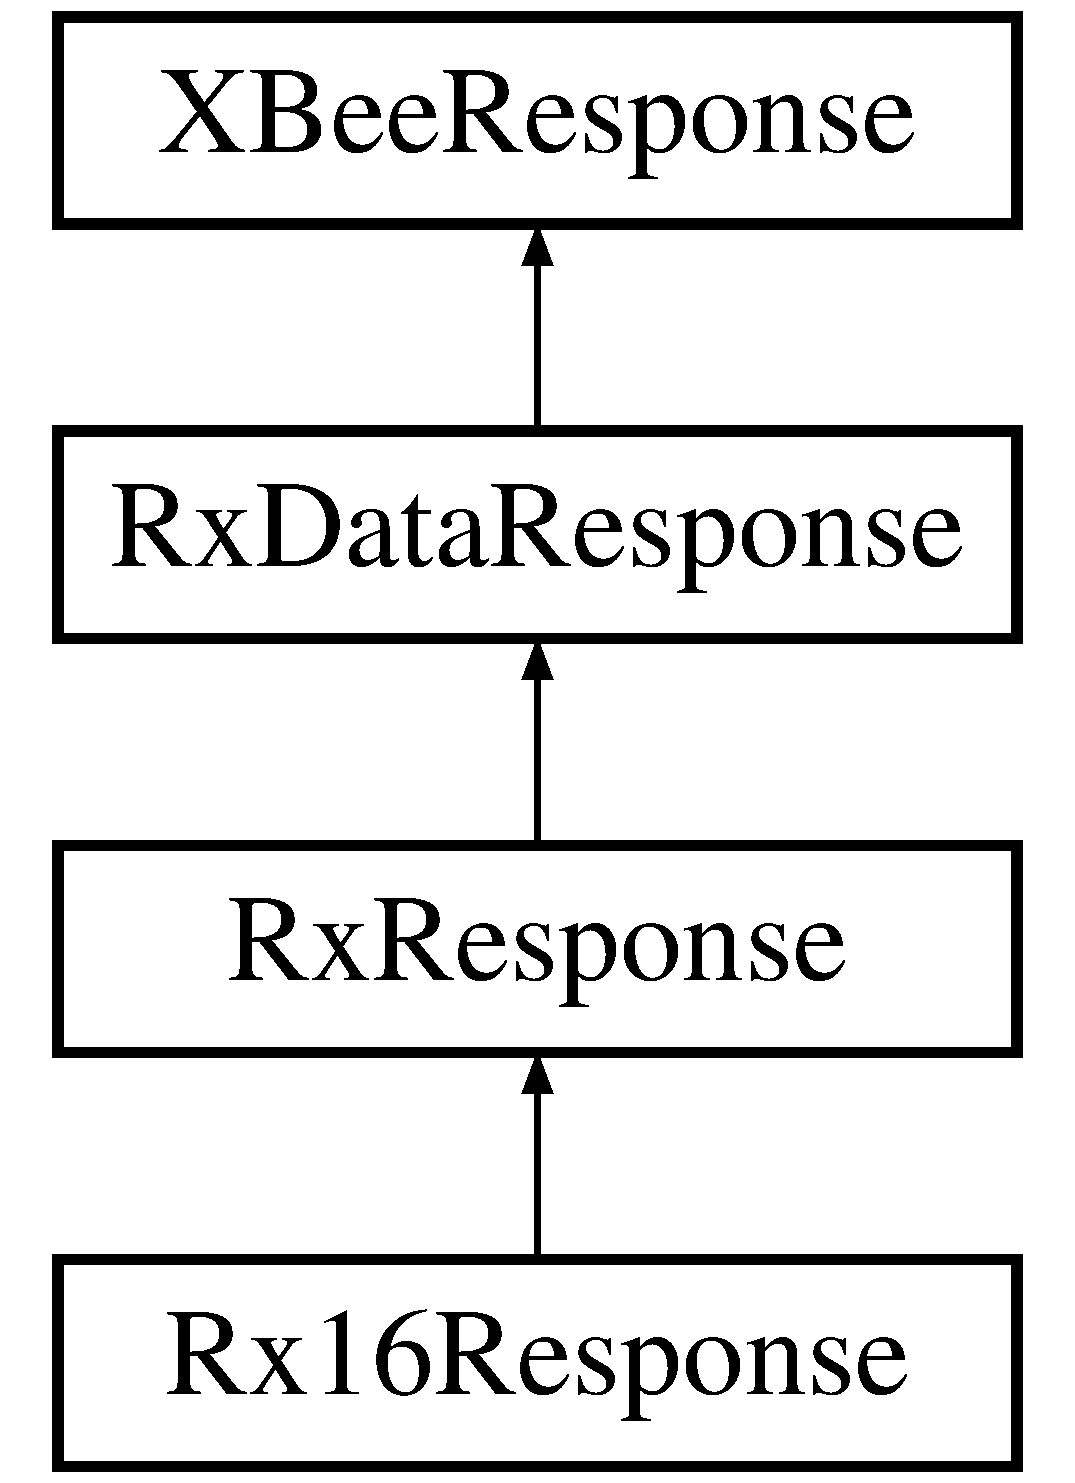
\includegraphics[height=4.000000cm]{classRx16Response}
\end{center}
\end{figure}
\subsection*{\-Public \-Member \-Functions}
\begin{DoxyCompactItemize}
\item 
\hypertarget{classRx16Response_ac63deea5667857ec74285daf5fab6328}{uint8\-\_\-t {\bfseries get\-Rssi\-Offset} ()}\label{classRx16Response_ac63deea5667857ec74285daf5fab6328}

\item 
\hypertarget{classRx16Response_abd8853ab7edcfa686000e81ce17983c4}{uint16\-\_\-t {\bfseries get\-Remote\-Address16} ()}\label{classRx16Response_abd8853ab7edcfa686000e81ce17983c4}

\end{DoxyCompactItemize}
\subsection*{\-Protected \-Attributes}
\begin{DoxyCompactItemize}
\item 
\hypertarget{classRx16Response_a8df57e3d897e22e4b6abdda7b2859123}{uint16\-\_\-t {\bfseries \-\_\-remote\-Address}}\label{classRx16Response_a8df57e3d897e22e4b6abdda7b2859123}

\end{DoxyCompactItemize}


\subsection{\-Detailed \-Description}
\-Represents a \-Series 1 16-\/bit address \-R\-X packet 

\-The documentation for this class was generated from the following files\-:\begin{DoxyCompactItemize}
\item 
\-X\-Bee.\-h\item 
\-X\-Bee.\-cpp\end{DoxyCompactItemize}

\hypertarget{classRx64IoSampleResponse}{\section{\-Rx64\-Io\-Sample\-Response \-Class \-Reference}
\label{classRx64IoSampleResponse}\index{\-Rx64\-Io\-Sample\-Response@{\-Rx64\-Io\-Sample\-Response}}
}
\-Inheritance diagram for \-Rx64\-Io\-Sample\-Response\-:\begin{figure}[H]
\begin{center}
\leavevmode
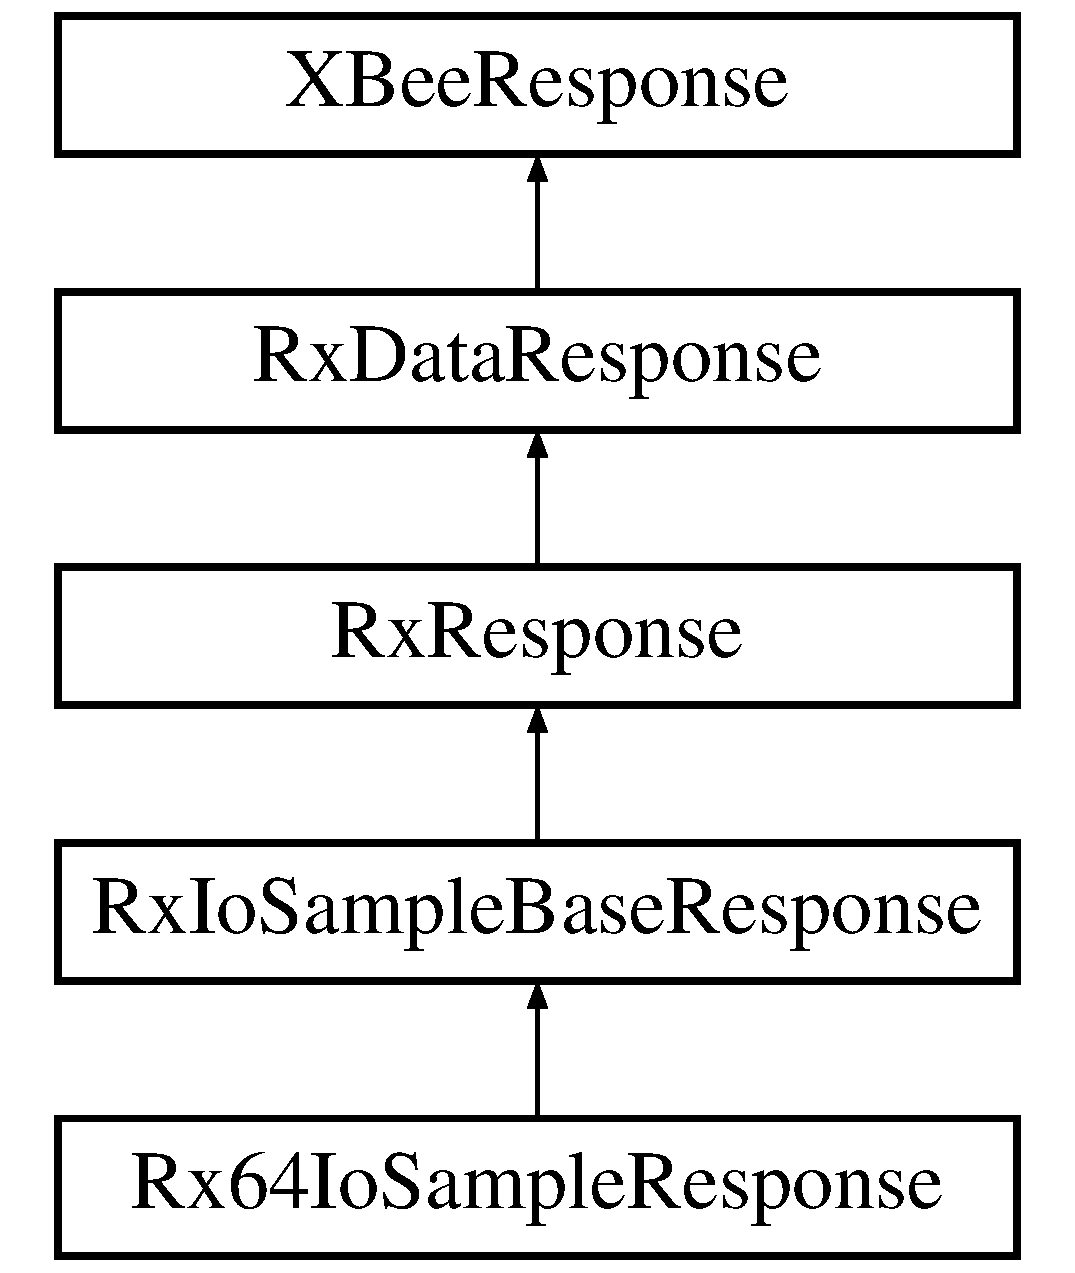
\includegraphics[height=5.000000cm]{classRx64IoSampleResponse}
\end{center}
\end{figure}
\subsection*{\-Public \-Member \-Functions}
\begin{DoxyCompactItemize}
\item 
\hypertarget{classRx64IoSampleResponse_a820798904df6b3bef202444e349f94dd}{\hyperlink{classXBeeAddress64}{\-X\-Bee\-Address64} \& {\bfseries get\-Remote\-Address64} ()}\label{classRx64IoSampleResponse_a820798904df6b3bef202444e349f94dd}

\item 
\hypertarget{classRx64IoSampleResponse_abd780d5ca68b8389c44371522f775eae}{uint8\-\_\-t {\bfseries get\-Rssi\-Offset} ()}\label{classRx64IoSampleResponse_abd780d5ca68b8389c44371522f775eae}

\end{DoxyCompactItemize}


\-The documentation for this class was generated from the following files\-:\begin{DoxyCompactItemize}
\item 
\-X\-Bee.\-h\item 
\-X\-Bee.\-cpp\end{DoxyCompactItemize}

\hypertarget{classRx64Response}{\section{\-Rx64\-Response \-Class \-Reference}
\label{classRx64Response}\index{\-Rx64\-Response@{\-Rx64\-Response}}
}


{\ttfamily \#include $<$\-X\-Bee.\-h$>$}

\-Inheritance diagram for \-Rx64\-Response\-:\begin{figure}[H]
\begin{center}
\leavevmode
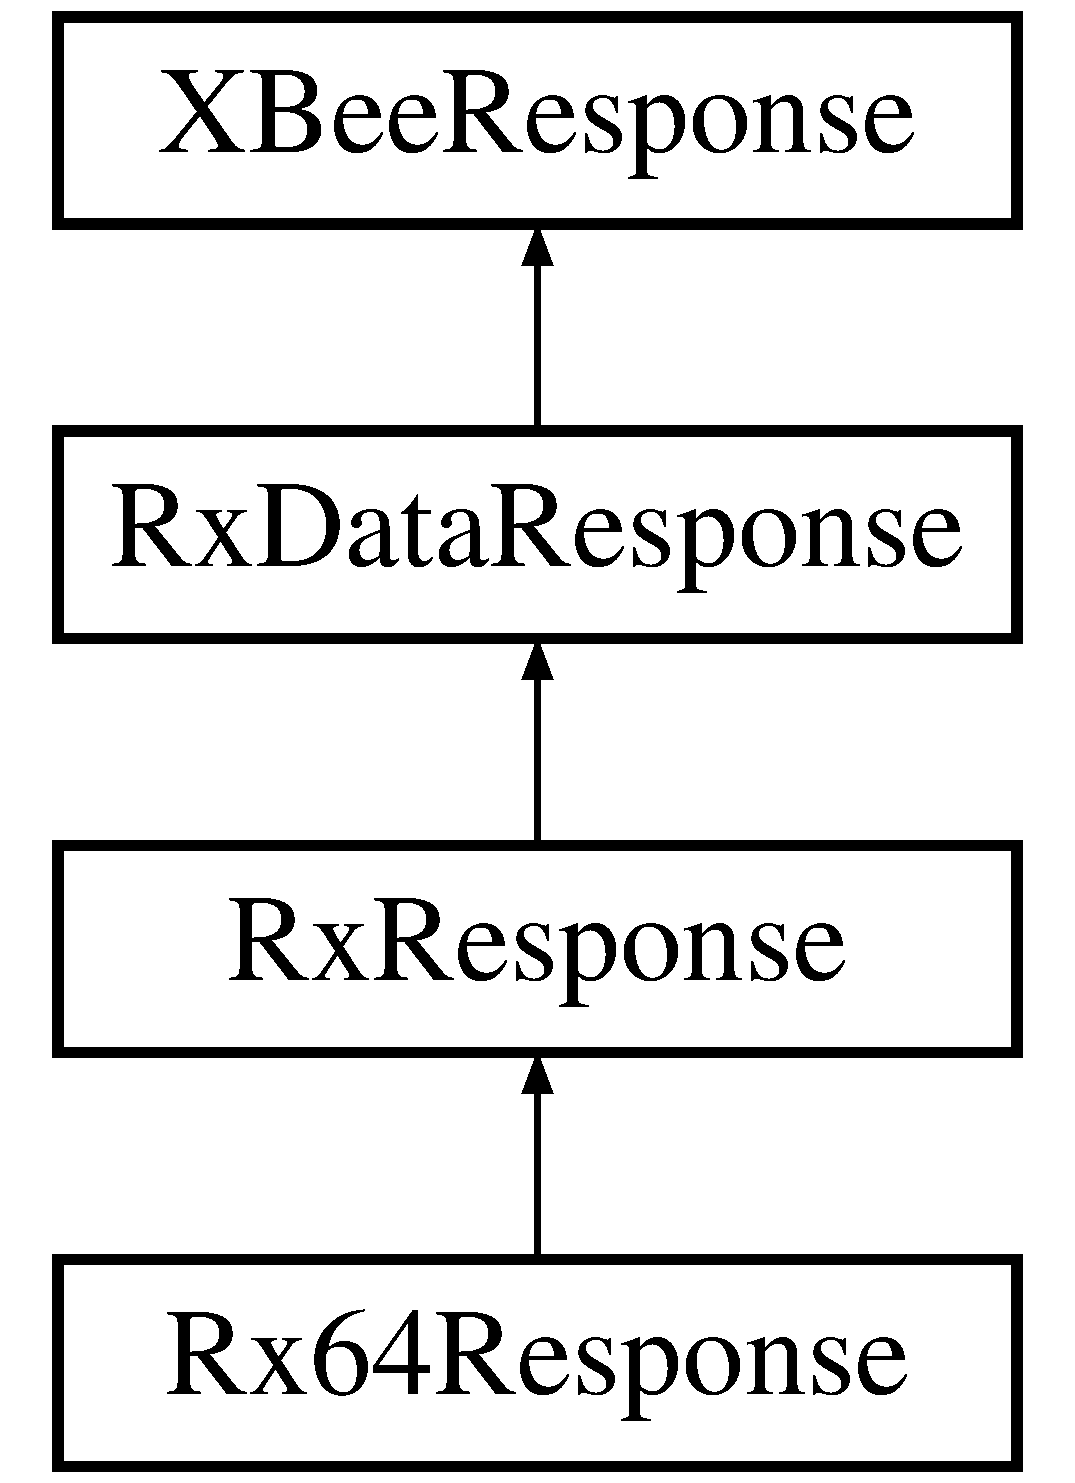
\includegraphics[height=4.000000cm]{classRx64Response}
\end{center}
\end{figure}
\subsection*{\-Public \-Member \-Functions}
\begin{DoxyCompactItemize}
\item 
\hypertarget{classRx64Response_a5540b8d71a920049bee9ced78b37798e}{uint8\-\_\-t {\bfseries get\-Rssi\-Offset} ()}\label{classRx64Response_a5540b8d71a920049bee9ced78b37798e}

\item 
\hypertarget{classRx64Response_aefd36322881280a6b5f26eca12c2dca6}{\hyperlink{classXBeeAddress64}{\-X\-Bee\-Address64} \& {\bfseries get\-Remote\-Address64} ()}\label{classRx64Response_aefd36322881280a6b5f26eca12c2dca6}

\end{DoxyCompactItemize}


\subsection{\-Detailed \-Description}
\-Represents a \-Series 1 64-\/bit address \-R\-X packet 

\-The documentation for this class was generated from the following files\-:\begin{DoxyCompactItemize}
\item 
\-X\-Bee.\-h\item 
\-X\-Bee.\-cpp\end{DoxyCompactItemize}

\hypertarget{classRxDataResponse}{\section{\-Rx\-Data\-Response \-Class \-Reference}
\label{classRxDataResponse}\index{\-Rx\-Data\-Response@{\-Rx\-Data\-Response}}
}


{\ttfamily \#include $<$\-X\-Bee.\-h$>$}

\-Inheritance diagram for \-Rx\-Data\-Response\-:\begin{figure}[H]
\begin{center}
\leavevmode
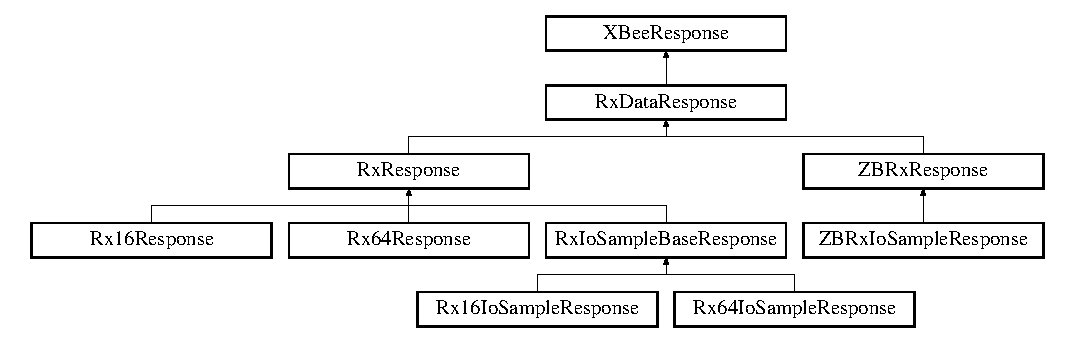
\includegraphics[height=4.166667cm]{classRxDataResponse}
\end{center}
\end{figure}
\subsection*{\-Public \-Member \-Functions}
\begin{DoxyCompactItemize}
\item 
uint8\-\_\-t \hyperlink{classRxDataResponse_a28db0306283f4191e4fc8a5b049486f5}{get\-Data} (int index)
\item 
uint8\-\_\-t $\ast$ \hyperlink{classRxDataResponse_ae0f858fe479a07c7122a8d414c60517e}{get\-Data} ()
\item 
virtual uint8\-\_\-t \hyperlink{classRxDataResponse_a5845e6a0719fd0bf52675e47053a704e}{get\-Data\-Length} ()=0
\item 
virtual uint8\-\_\-t \hyperlink{classRxDataResponse_a9e4b6bf4f1bfd9ccec45d190a204f61a}{get\-Data\-Offset} ()=0
\end{DoxyCompactItemize}


\subsection{\-Detailed \-Description}
\-Common functionality for both \-Series 1 and 2 data \-R\-X data packets 

\subsection{\-Member \-Function \-Documentation}
\hypertarget{classRxDataResponse_a28db0306283f4191e4fc8a5b049486f5}{\index{\-Rx\-Data\-Response@{\-Rx\-Data\-Response}!get\-Data@{get\-Data}}
\index{get\-Data@{get\-Data}!RxDataResponse@{\-Rx\-Data\-Response}}
\subsubsection[{get\-Data}]{\setlength{\rightskip}{0pt plus 5cm}uint8\-\_\-t {\bf \-Rx\-Data\-Response\-::get\-Data} (
\begin{DoxyParamCaption}
\item[{int}]{index}
\end{DoxyParamCaption}
)}}\label{classRxDataResponse_a28db0306283f4191e4fc8a5b049486f5}
\-Returns the specified index of the payload. \-The index may be 0 to \hyperlink{classRxDataResponse_a5845e6a0719fd0bf52675e47053a704e}{get\-Data\-Length()} -\/ 1 \-This method is deprecated; use uint8\-\_\-t$\ast$ \hyperlink{classRxDataResponse_ae0f858fe479a07c7122a8d414c60517e}{get\-Data()} \hypertarget{classRxDataResponse_ae0f858fe479a07c7122a8d414c60517e}{\index{\-Rx\-Data\-Response@{\-Rx\-Data\-Response}!get\-Data@{get\-Data}}
\index{get\-Data@{get\-Data}!RxDataResponse@{\-Rx\-Data\-Response}}
\subsubsection[{get\-Data}]{\setlength{\rightskip}{0pt plus 5cm}uint8\-\_\-t $\ast$ {\bf \-Rx\-Data\-Response\-::get\-Data} (
\begin{DoxyParamCaption}
{}
\end{DoxyParamCaption}
)}}\label{classRxDataResponse_ae0f858fe479a07c7122a8d414c60517e}
\-Returns the payload array. \-This may be accessed from index 0 to \hyperlink{classRxDataResponse_a5845e6a0719fd0bf52675e47053a704e}{get\-Data\-Length()} -\/ 1 \hypertarget{classRxDataResponse_a5845e6a0719fd0bf52675e47053a704e}{\index{\-Rx\-Data\-Response@{\-Rx\-Data\-Response}!get\-Data\-Length@{get\-Data\-Length}}
\index{get\-Data\-Length@{get\-Data\-Length}!RxDataResponse@{\-Rx\-Data\-Response}}
\subsubsection[{get\-Data\-Length}]{\setlength{\rightskip}{0pt plus 5cm}virtual uint8\-\_\-t {\bf \-Rx\-Data\-Response\-::get\-Data\-Length} (
\begin{DoxyParamCaption}
{}
\end{DoxyParamCaption}
)\hspace{0.3cm}{\ttfamily  \mbox{[}pure virtual\mbox{]}}}}\label{classRxDataResponse_a5845e6a0719fd0bf52675e47053a704e}
\-Returns the length of the payload 

\-Implemented in \hyperlink{classRxResponse_add3478a1ce5667aad315f6a6c218011a}{\-Rx\-Response}, and \hyperlink{classZBRxResponse_a9d2b73060d611bbdd581e0ceb195fd31}{\-Z\-B\-Rx\-Response}.

\hypertarget{classRxDataResponse_a9e4b6bf4f1bfd9ccec45d190a204f61a}{\index{\-Rx\-Data\-Response@{\-Rx\-Data\-Response}!get\-Data\-Offset@{get\-Data\-Offset}}
\index{get\-Data\-Offset@{get\-Data\-Offset}!RxDataResponse@{\-Rx\-Data\-Response}}
\subsubsection[{get\-Data\-Offset}]{\setlength{\rightskip}{0pt plus 5cm}virtual uint8\-\_\-t {\bf \-Rx\-Data\-Response\-::get\-Data\-Offset} (
\begin{DoxyParamCaption}
{}
\end{DoxyParamCaption}
)\hspace{0.3cm}{\ttfamily  \mbox{[}pure virtual\mbox{]}}}}\label{classRxDataResponse_a9e4b6bf4f1bfd9ccec45d190a204f61a}
\-Returns the position in the frame data where the data begins 

\-Implemented in \hyperlink{classRxResponse_a37fd3ee455f2157fa3894e710e668409}{\-Rx\-Response}, and \hyperlink{classZBRxResponse_ad54e6ff3008f79d0ed32a78cc3d69151}{\-Z\-B\-Rx\-Response}.



\-The documentation for this class was generated from the following files\-:\begin{DoxyCompactItemize}
\item 
\-X\-Bee.\-h\item 
\-X\-Bee.\-cpp\end{DoxyCompactItemize}

\hypertarget{classRxIoSampleBaseResponse}{\section{\-Rx\-Io\-Sample\-Base\-Response \-Class \-Reference}
\label{classRxIoSampleBaseResponse}\index{\-Rx\-Io\-Sample\-Base\-Response@{\-Rx\-Io\-Sample\-Base\-Response}}
}


{\ttfamily \#include $<$\-X\-Bee.\-h$>$}

\-Inheritance diagram for \-Rx\-Io\-Sample\-Base\-Response\-:\begin{figure}[H]
\begin{center}
\leavevmode
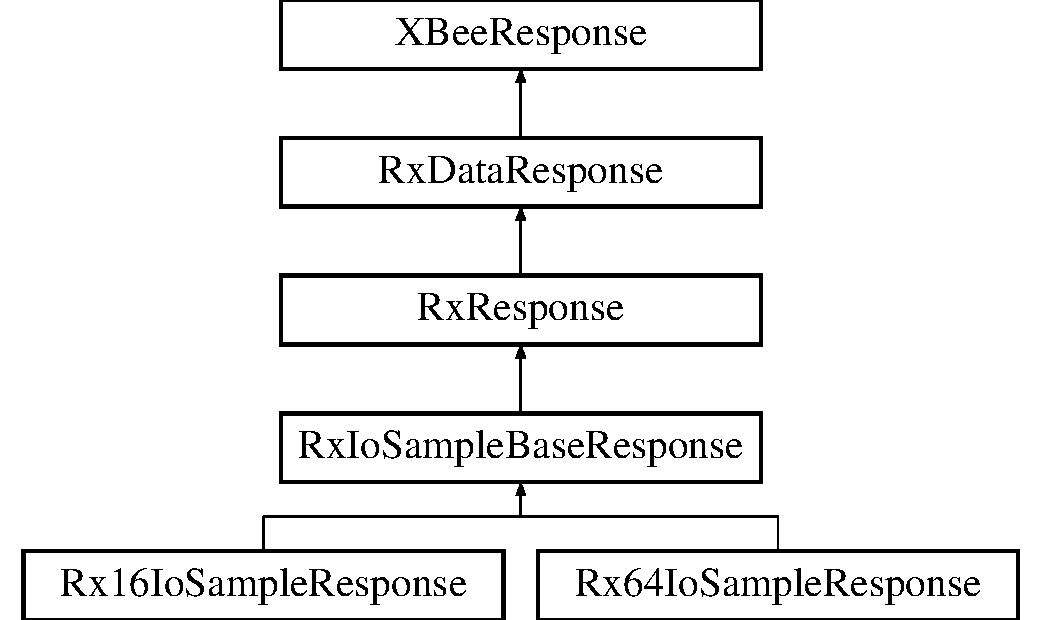
\includegraphics[height=5.000000cm]{classRxIoSampleBaseResponse}
\end{center}
\end{figure}
\subsection*{\-Public \-Member \-Functions}
\begin{DoxyCompactItemize}
\item 
uint8\-\_\-t \hyperlink{classRxIoSampleBaseResponse_a44ce66a6751e7e39c8908fe179a21d24}{get\-Sample\-Size} ()
\item 
\hypertarget{classRxIoSampleBaseResponse_a9c6f6e1b7b8659ea086084ca35f9f83b}{bool {\bfseries contains\-Analog} ()}\label{classRxIoSampleBaseResponse_a9c6f6e1b7b8659ea086084ca35f9f83b}

\item 
\hypertarget{classRxIoSampleBaseResponse_ae70a93197c9e2fa6cfd5d64e189f0690}{bool {\bfseries contains\-Digital} ()}\label{classRxIoSampleBaseResponse_ae70a93197c9e2fa6cfd5d64e189f0690}

\item 
bool \hyperlink{classRxIoSampleBaseResponse_ad8fc07932c2e011b83814082b1d82400}{is\-Analog\-Enabled} (uint8\-\_\-t pin)
\item 
bool \hyperlink{classRxIoSampleBaseResponse_aa897267985b5b8c02abd68b50f954de7}{is\-Digital\-Enabled} (uint8\-\_\-t pin)
\item 
uint16\-\_\-t \hyperlink{classRxIoSampleBaseResponse_a81e98b2eab33f62e6af6b3b4014e841a}{get\-Analog} (uint8\-\_\-t pin, uint8\-\_\-t sample)
\item 
bool \hyperlink{classRxIoSampleBaseResponse_ad4ffc0eb84c685fe45618d6b73a20ce2}{is\-Digital\-On} (uint8\-\_\-t pin, uint8\-\_\-t sample)
\item 
\hypertarget{classRxIoSampleBaseResponse_a78098028dec69c655a190fb8d3cee333}{uint8\-\_\-t {\bfseries get\-Sample\-Offset} ()}\label{classRxIoSampleBaseResponse_a78098028dec69c655a190fb8d3cee333}

\end{DoxyCompactItemize}


\subsection{\-Detailed \-Description}
\-Represents a \-Series 1 \-R\-X \-I/\-O \-Sample packet 

\subsection{\-Member \-Function \-Documentation}
\hypertarget{classRxIoSampleBaseResponse_a81e98b2eab33f62e6af6b3b4014e841a}{\index{\-Rx\-Io\-Sample\-Base\-Response@{\-Rx\-Io\-Sample\-Base\-Response}!get\-Analog@{get\-Analog}}
\index{get\-Analog@{get\-Analog}!RxIoSampleBaseResponse@{\-Rx\-Io\-Sample\-Base\-Response}}
\subsubsection[{get\-Analog}]{\setlength{\rightskip}{0pt plus 5cm}uint16\-\_\-t {\bf \-Rx\-Io\-Sample\-Base\-Response\-::get\-Analog} (
\begin{DoxyParamCaption}
\item[{uint8\-\_\-t}]{pin, }
\item[{uint8\-\_\-t}]{sample}
\end{DoxyParamCaption}
)}}\label{classRxIoSampleBaseResponse_a81e98b2eab33f62e6af6b3b4014e841a}
\-Returns the 10-\/bit analog reading of the specified pin. \-Valid pins include \-A\-D\-C\-:0-\/5. \-Sample index starts at 0 \hypertarget{classRxIoSampleBaseResponse_a44ce66a6751e7e39c8908fe179a21d24}{\index{\-Rx\-Io\-Sample\-Base\-Response@{\-Rx\-Io\-Sample\-Base\-Response}!get\-Sample\-Size@{get\-Sample\-Size}}
\index{get\-Sample\-Size@{get\-Sample\-Size}!RxIoSampleBaseResponse@{\-Rx\-Io\-Sample\-Base\-Response}}
\subsubsection[{get\-Sample\-Size}]{\setlength{\rightskip}{0pt plus 5cm}uint8\-\_\-t {\bf \-Rx\-Io\-Sample\-Base\-Response\-::get\-Sample\-Size} (
\begin{DoxyParamCaption}
{}
\end{DoxyParamCaption}
)}}\label{classRxIoSampleBaseResponse_a44ce66a6751e7e39c8908fe179a21d24}
\-Returns the number of samples in this packet \hypertarget{classRxIoSampleBaseResponse_ad8fc07932c2e011b83814082b1d82400}{\index{\-Rx\-Io\-Sample\-Base\-Response@{\-Rx\-Io\-Sample\-Base\-Response}!is\-Analog\-Enabled@{is\-Analog\-Enabled}}
\index{is\-Analog\-Enabled@{is\-Analog\-Enabled}!RxIoSampleBaseResponse@{\-Rx\-Io\-Sample\-Base\-Response}}
\subsubsection[{is\-Analog\-Enabled}]{\setlength{\rightskip}{0pt plus 5cm}bool {\bf \-Rx\-Io\-Sample\-Base\-Response\-::is\-Analog\-Enabled} (
\begin{DoxyParamCaption}
\item[{uint8\-\_\-t}]{pin}
\end{DoxyParamCaption}
)}}\label{classRxIoSampleBaseResponse_ad8fc07932c2e011b83814082b1d82400}
\-Returns true if the specified analog pin is enabled \hypertarget{classRxIoSampleBaseResponse_aa897267985b5b8c02abd68b50f954de7}{\index{\-Rx\-Io\-Sample\-Base\-Response@{\-Rx\-Io\-Sample\-Base\-Response}!is\-Digital\-Enabled@{is\-Digital\-Enabled}}
\index{is\-Digital\-Enabled@{is\-Digital\-Enabled}!RxIoSampleBaseResponse@{\-Rx\-Io\-Sample\-Base\-Response}}
\subsubsection[{is\-Digital\-Enabled}]{\setlength{\rightskip}{0pt plus 5cm}bool {\bf \-Rx\-Io\-Sample\-Base\-Response\-::is\-Digital\-Enabled} (
\begin{DoxyParamCaption}
\item[{uint8\-\_\-t}]{pin}
\end{DoxyParamCaption}
)}}\label{classRxIoSampleBaseResponse_aa897267985b5b8c02abd68b50f954de7}
\-Returns true if the specified digital pin is enabled \hypertarget{classRxIoSampleBaseResponse_ad4ffc0eb84c685fe45618d6b73a20ce2}{\index{\-Rx\-Io\-Sample\-Base\-Response@{\-Rx\-Io\-Sample\-Base\-Response}!is\-Digital\-On@{is\-Digital\-On}}
\index{is\-Digital\-On@{is\-Digital\-On}!RxIoSampleBaseResponse@{\-Rx\-Io\-Sample\-Base\-Response}}
\subsubsection[{is\-Digital\-On}]{\setlength{\rightskip}{0pt plus 5cm}bool {\bf \-Rx\-Io\-Sample\-Base\-Response\-::is\-Digital\-On} (
\begin{DoxyParamCaption}
\item[{uint8\-\_\-t}]{pin, }
\item[{uint8\-\_\-t}]{sample}
\end{DoxyParamCaption}
)}}\label{classRxIoSampleBaseResponse_ad4ffc0eb84c685fe45618d6b73a20ce2}
\-Returns true if the specified pin is high/on. \-Valid pins include \-D\-I\-O\-:0-\/8. \-Sample index starts at 0 

\-The documentation for this class was generated from the following files\-:\begin{DoxyCompactItemize}
\item 
\-X\-Bee.\-h\item 
\-X\-Bee.\-cpp\end{DoxyCompactItemize}

\hypertarget{classRxResponse}{\section{\-Rx\-Response \-Class \-Reference}
\label{classRxResponse}\index{\-Rx\-Response@{\-Rx\-Response}}
}


{\ttfamily \#include $<$\-X\-Bee.\-h$>$}

\-Inheritance diagram for \-Rx\-Response\-:\begin{figure}[H]
\begin{center}
\leavevmode
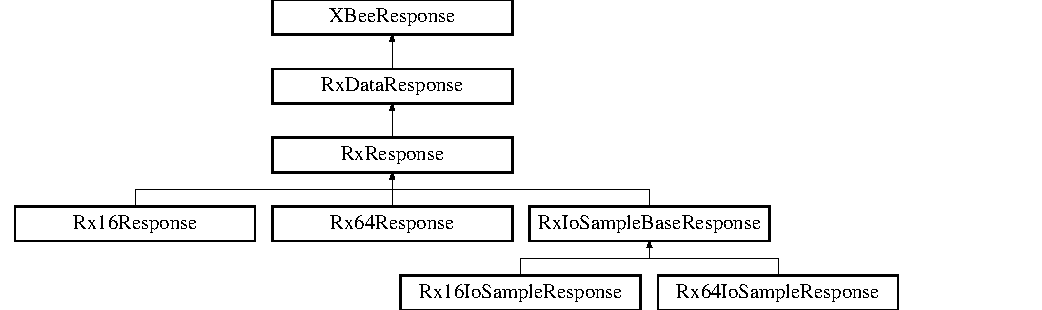
\includegraphics[height=4.166667cm]{classRxResponse}
\end{center}
\end{figure}
\subsection*{\-Public \-Member \-Functions}
\begin{DoxyCompactItemize}
\item 
\hypertarget{classRxResponse_a43fa3b1d0f4df2491496d10d7981799e}{uint8\-\_\-t {\bfseries get\-Rssi} ()}\label{classRxResponse_a43fa3b1d0f4df2491496d10d7981799e}

\item 
\hypertarget{classRxResponse_a1bd75535804b6c1ff64a9ecd8aba6fcd}{uint8\-\_\-t {\bfseries get\-Option} ()}\label{classRxResponse_a1bd75535804b6c1ff64a9ecd8aba6fcd}

\item 
\hypertarget{classRxResponse_ac85e73bfa6656b2c96275101e6fdea6e}{bool {\bfseries is\-Address\-Broadcast} ()}\label{classRxResponse_ac85e73bfa6656b2c96275101e6fdea6e}

\item 
\hypertarget{classRxResponse_a1b492ad1ff869b00903efc4ff571a006}{bool {\bfseries is\-Pan\-Broadcast} ()}\label{classRxResponse_a1b492ad1ff869b00903efc4ff571a006}

\item 
uint8\-\_\-t \hyperlink{classRxResponse_add3478a1ce5667aad315f6a6c218011a}{get\-Data\-Length} ()
\item 
uint8\-\_\-t \hyperlink{classRxResponse_a37fd3ee455f2157fa3894e710e668409}{get\-Data\-Offset} ()
\item 
\hypertarget{classRxResponse_ac0e5dc8fc16aa3004b5c59a8a306e00e}{virtual uint8\-\_\-t {\bfseries get\-Rssi\-Offset} ()=0}\label{classRxResponse_ac0e5dc8fc16aa3004b5c59a8a306e00e}

\end{DoxyCompactItemize}


\subsection{\-Detailed \-Description}
\-Represents a \-Series 1 \-R\-X packet 

\subsection{\-Member \-Function \-Documentation}
\hypertarget{classRxResponse_add3478a1ce5667aad315f6a6c218011a}{\index{\-Rx\-Response@{\-Rx\-Response}!get\-Data\-Length@{get\-Data\-Length}}
\index{get\-Data\-Length@{get\-Data\-Length}!RxResponse@{\-Rx\-Response}}
\subsubsection[{get\-Data\-Length}]{\setlength{\rightskip}{0pt plus 5cm}uint8\-\_\-t {\bf \-Rx\-Response\-::get\-Data\-Length} (
\begin{DoxyParamCaption}
{}
\end{DoxyParamCaption}
)\hspace{0.3cm}{\ttfamily  \mbox{[}virtual\mbox{]}}}}\label{classRxResponse_add3478a1ce5667aad315f6a6c218011a}
\-Returns the length of the payload 

\-Implements \hyperlink{classRxDataResponse_a5845e6a0719fd0bf52675e47053a704e}{\-Rx\-Data\-Response}.

\hypertarget{classRxResponse_a37fd3ee455f2157fa3894e710e668409}{\index{\-Rx\-Response@{\-Rx\-Response}!get\-Data\-Offset@{get\-Data\-Offset}}
\index{get\-Data\-Offset@{get\-Data\-Offset}!RxResponse@{\-Rx\-Response}}
\subsubsection[{get\-Data\-Offset}]{\setlength{\rightskip}{0pt plus 5cm}uint8\-\_\-t {\bf \-Rx\-Response\-::get\-Data\-Offset} (
\begin{DoxyParamCaption}
{}
\end{DoxyParamCaption}
)\hspace{0.3cm}{\ttfamily  \mbox{[}virtual\mbox{]}}}}\label{classRxResponse_a37fd3ee455f2157fa3894e710e668409}
\-Returns the position in the frame data where the data begins 

\-Implements \hyperlink{classRxDataResponse_a9e4b6bf4f1bfd9ccec45d190a204f61a}{\-Rx\-Data\-Response}.



\-The documentation for this class was generated from the following files\-:\begin{DoxyCompactItemize}
\item 
\-X\-Bee.\-h\item 
\-X\-Bee.\-cpp\end{DoxyCompactItemize}

\hypertarget{classTx16Request}{\section{\-Tx16\-Request \-Class \-Reference}
\label{classTx16Request}\index{\-Tx16\-Request@{\-Tx16\-Request}}
}


{\ttfamily \#include $<$\-X\-Bee.\-h$>$}

\-Inheritance diagram for \-Tx16\-Request\-:\begin{figure}[H]
\begin{center}
\leavevmode
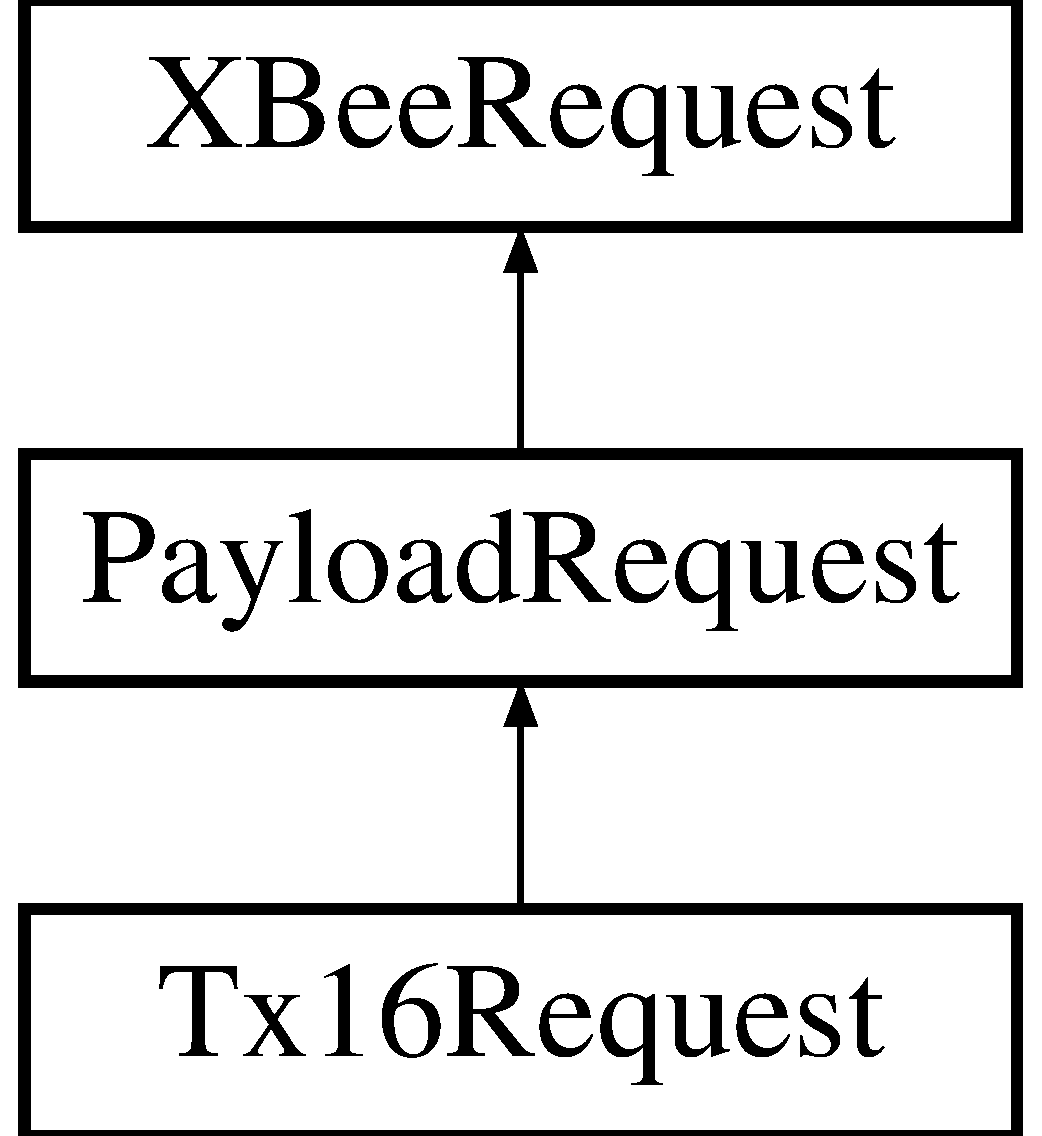
\includegraphics[height=3.000000cm]{classTx16Request}
\end{center}
\end{figure}
\subsection*{\-Public \-Member \-Functions}
\begin{DoxyCompactItemize}
\item 
\hypertarget{classTx16Request_a4e8f8b660e4837f4053e9f18d394f913}{{\bfseries \-Tx16\-Request} (uint16\-\_\-t addr16, uint8\-\_\-t option, uint8\-\_\-t $\ast$payload, uint8\-\_\-t payload\-Length, uint8\-\_\-t frame\-Id)}\label{classTx16Request_a4e8f8b660e4837f4053e9f18d394f913}

\item 
\hyperlink{classTx16Request_a760e2c31996673e816fb3576748f731f}{\-Tx16\-Request} (uint16\-\_\-t addr16, uint8\-\_\-t $\ast$payload, uint8\-\_\-t payload\-Length)
\item 
\hyperlink{classTx16Request_adcdbb644e08788267fb86cbefde76b1b}{\-Tx16\-Request} ()
\item 
\hypertarget{classTx16Request_adeb9cf2989e2c86992f6a652a92bd648}{uint16\-\_\-t {\bfseries get\-Address16} ()}\label{classTx16Request_adeb9cf2989e2c86992f6a652a92bd648}

\item 
\hypertarget{classTx16Request_ac28c597252a64d47df3bb61dd8251ee4}{void {\bfseries set\-Address16} (uint16\-\_\-t addr16)}\label{classTx16Request_ac28c597252a64d47df3bb61dd8251ee4}

\item 
\hypertarget{classTx16Request_a448d4a28812d6cc67a7c45138ba6061c}{uint8\-\_\-t {\bfseries get\-Option} ()}\label{classTx16Request_a448d4a28812d6cc67a7c45138ba6061c}

\item 
\hypertarget{classTx16Request_afc0792e586ddb3c9d62efb787a5956d9}{void {\bfseries set\-Option} (uint8\-\_\-t option)}\label{classTx16Request_afc0792e586ddb3c9d62efb787a5956d9}

\item 
uint8\-\_\-t \hyperlink{classTx16Request_af5ffbc2164e766d96f54c723996fd389}{get\-Frame\-Data} (uint8\-\_\-t pos)
\item 
uint8\-\_\-t \hyperlink{classTx16Request_a9a1ddfb380e72ecc09a024c6de6cdf8e}{get\-Frame\-Data\-Length} ()
\end{DoxyCompactItemize}


\subsection{\-Detailed \-Description}
\-Represents a \-Series 1 \-T\-X packet that corresponds to \-Api \-Id\-: \-T\-X\-\_\-16\-\_\-\-R\-E\-Q\-U\-E\-S\-T 

\-Be careful not to send a data array larger than the max packet size of your radio. \-This class does not perform any validation of packet size and there will be no indication if the packet is too large, other than you will not get a \-T\-X \-Status response. \-The datasheet says 100 bytes is the maximum, although that could change in future firmware. 

\subsection{\-Constructor \& \-Destructor \-Documentation}
\hypertarget{classTx16Request_a760e2c31996673e816fb3576748f731f}{\index{\-Tx16\-Request@{\-Tx16\-Request}!\-Tx16\-Request@{\-Tx16\-Request}}
\index{\-Tx16\-Request@{\-Tx16\-Request}!Tx16Request@{\-Tx16\-Request}}
\subsubsection[{\-Tx16\-Request}]{\setlength{\rightskip}{0pt plus 5cm}\-Tx16\-Request\-::\-Tx16\-Request (
\begin{DoxyParamCaption}
\item[{uint16\-\_\-t}]{addr16, }
\item[{uint8\-\_\-t $\ast$}]{payload, }
\item[{uint8\-\_\-t}]{payload\-Length}
\end{DoxyParamCaption}
)}}\label{classTx16Request_a760e2c31996673e816fb3576748f731f}
\-Creates a \-Unicast \hyperlink{classTx16Request}{\-Tx16\-Request} with the \-A\-C\-K option and \-D\-E\-F\-A\-U\-L\-T\-\_\-\-F\-R\-A\-M\-E\-\_\-\-I\-D \hypertarget{classTx16Request_adcdbb644e08788267fb86cbefde76b1b}{\index{\-Tx16\-Request@{\-Tx16\-Request}!\-Tx16\-Request@{\-Tx16\-Request}}
\index{\-Tx16\-Request@{\-Tx16\-Request}!Tx16Request@{\-Tx16\-Request}}
\subsubsection[{\-Tx16\-Request}]{\setlength{\rightskip}{0pt plus 5cm}\-Tx16\-Request\-::\-Tx16\-Request (
\begin{DoxyParamCaption}
{}
\end{DoxyParamCaption}
)}}\label{classTx16Request_adcdbb644e08788267fb86cbefde76b1b}
\-Creates a default instance of this class. \-At a minimum you must specify a payload, payload length and a destination address before sending this request. 

\subsection{\-Member \-Function \-Documentation}
\hypertarget{classTx16Request_af5ffbc2164e766d96f54c723996fd389}{\index{\-Tx16\-Request@{\-Tx16\-Request}!get\-Frame\-Data@{get\-Frame\-Data}}
\index{get\-Frame\-Data@{get\-Frame\-Data}!Tx16Request@{\-Tx16\-Request}}
\subsubsection[{get\-Frame\-Data}]{\setlength{\rightskip}{0pt plus 5cm}uint8\-\_\-t {\bf \-Tx16\-Request\-::get\-Frame\-Data} (
\begin{DoxyParamCaption}
\item[{uint8\-\_\-t}]{pos}
\end{DoxyParamCaption}
)\hspace{0.3cm}{\ttfamily  \mbox{[}virtual\mbox{]}}}}\label{classTx16Request_af5ffbc2164e766d96f54c723996fd389}
\-Starting after the frame id (pos = 0) and up to but not including the checksum \-Note\-: \-Unlike \-Digi's definition of the frame data, this does not start with the \-A\-P\-I \-I\-D. \-The reason for this is the \-A\-P\-I \-I\-D and \-Frame \-I\-D are common to all requests, whereas my definition of frame data is only the \-A\-P\-I specific data. 

\-Implements \hyperlink{classXBeeRequest_ad5b998cd95a570bdaa4d74c6c8790d94}{\-X\-Bee\-Request}.

\hypertarget{classTx16Request_a9a1ddfb380e72ecc09a024c6de6cdf8e}{\index{\-Tx16\-Request@{\-Tx16\-Request}!get\-Frame\-Data\-Length@{get\-Frame\-Data\-Length}}
\index{get\-Frame\-Data\-Length@{get\-Frame\-Data\-Length}!Tx16Request@{\-Tx16\-Request}}
\subsubsection[{get\-Frame\-Data\-Length}]{\setlength{\rightskip}{0pt plus 5cm}uint8\-\_\-t {\bf \-Tx16\-Request\-::get\-Frame\-Data\-Length} (
\begin{DoxyParamCaption}
{}
\end{DoxyParamCaption}
)\hspace{0.3cm}{\ttfamily  \mbox{[}virtual\mbox{]}}}}\label{classTx16Request_a9a1ddfb380e72ecc09a024c6de6cdf8e}
\-Returns the size of the api frame (not including frame id or api id or checksum). 

\-Implements \hyperlink{classXBeeRequest_a03b6c558db5836fa7167c0fba7405642}{\-X\-Bee\-Request}.



\-The documentation for this class was generated from the following files\-:\begin{DoxyCompactItemize}
\item 
\-X\-Bee.\-h\item 
\-X\-Bee.\-cpp\end{DoxyCompactItemize}

\hypertarget{classTx64Request}{\section{\-Tx64\-Request \-Class \-Reference}
\label{classTx64Request}\index{\-Tx64\-Request@{\-Tx64\-Request}}
}


{\ttfamily \#include $<$\-X\-Bee.\-h$>$}

\-Inheritance diagram for \-Tx64\-Request\-:\begin{figure}[H]
\begin{center}
\leavevmode
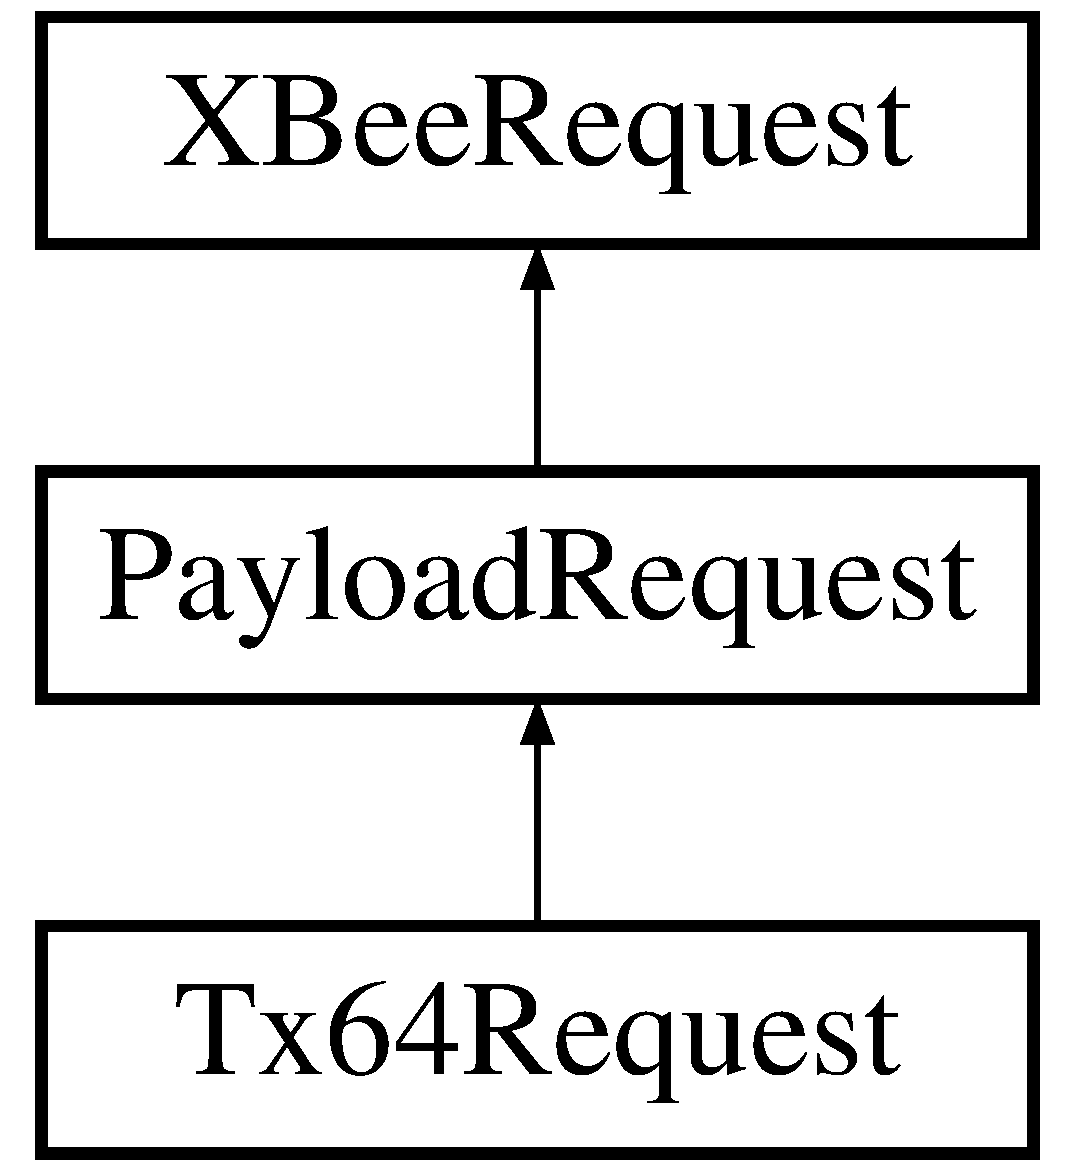
\includegraphics[height=3.000000cm]{classTx64Request}
\end{center}
\end{figure}
\subsection*{\-Public \-Member \-Functions}
\begin{DoxyCompactItemize}
\item 
\hypertarget{classTx64Request_a7670fd44d8765d8215a3e5cfcf605c1e}{{\bfseries \-Tx64\-Request} (\hyperlink{classXBeeAddress64}{\-X\-Bee\-Address64} \&addr64, uint8\-\_\-t option, uint8\-\_\-t $\ast$payload, uint8\-\_\-t payload\-Length, uint8\-\_\-t frame\-Id)}\label{classTx64Request_a7670fd44d8765d8215a3e5cfcf605c1e}

\item 
\hyperlink{classTx64Request_a7c9d830fa804daaf39ed368894cf9691}{\-Tx64\-Request} (\hyperlink{classXBeeAddress64}{\-X\-Bee\-Address64} \&addr64, uint8\-\_\-t $\ast$payload, uint8\-\_\-t payload\-Length)
\item 
\hyperlink{classTx64Request_a49bd84b4aa5478c27e6da5581b2e1d3c}{\-Tx64\-Request} ()
\item 
\hypertarget{classTx64Request_a8f6970aa54b8504be65e05ce1f52e8e4}{\hyperlink{classXBeeAddress64}{\-X\-Bee\-Address64} \& {\bfseries get\-Address64} ()}\label{classTx64Request_a8f6970aa54b8504be65e05ce1f52e8e4}

\item 
\hypertarget{classTx64Request_a863a993ad01c08b5c9835e9d7288bedd}{void {\bfseries set\-Address64} (\hyperlink{classXBeeAddress64}{\-X\-Bee\-Address64} \&addr64)}\label{classTx64Request_a863a993ad01c08b5c9835e9d7288bedd}

\item 
\hypertarget{classTx64Request_aac90589d46191868f19713aea49a421f}{uint8\-\_\-t {\bfseries get\-Option} ()}\label{classTx64Request_aac90589d46191868f19713aea49a421f}

\item 
\hypertarget{classTx64Request_a7f6987e3910d97dd8f77f58184dc17c9}{void {\bfseries set\-Option} (uint8\-\_\-t option)}\label{classTx64Request_a7f6987e3910d97dd8f77f58184dc17c9}

\item 
uint8\-\_\-t \hyperlink{classTx64Request_afe3662433da85acd21f8a3d90844a084}{get\-Frame\-Data} (uint8\-\_\-t pos)
\item 
uint8\-\_\-t \hyperlink{classTx64Request_afadc1e07718a62d6c5a75a4bb07dfaae}{get\-Frame\-Data\-Length} ()
\end{DoxyCompactItemize}


\subsection{\-Detailed \-Description}
\-Represents a \-Series 1 \-T\-X packet that corresponds to \-Api \-Id\-: \-T\-X\-\_\-64\-\_\-\-R\-E\-Q\-U\-E\-S\-T

\-Be careful not to send a data array larger than the max packet size of your radio. \-This class does not perform any validation of packet size and there will be no indication if the packet is too large, other than you will not get a \-T\-X \-Status response. \-The datasheet says 100 bytes is the maximum, although that could change in future firmware. 

\subsection{\-Constructor \& \-Destructor \-Documentation}
\hypertarget{classTx64Request_a7c9d830fa804daaf39ed368894cf9691}{\index{\-Tx64\-Request@{\-Tx64\-Request}!\-Tx64\-Request@{\-Tx64\-Request}}
\index{\-Tx64\-Request@{\-Tx64\-Request}!Tx64Request@{\-Tx64\-Request}}
\subsubsection[{\-Tx64\-Request}]{\setlength{\rightskip}{0pt plus 5cm}\-Tx64\-Request\-::\-Tx64\-Request (
\begin{DoxyParamCaption}
\item[{{\bf \-X\-Bee\-Address64} \&}]{addr64, }
\item[{uint8\-\_\-t $\ast$}]{payload, }
\item[{uint8\-\_\-t}]{payload\-Length}
\end{DoxyParamCaption}
)}}\label{classTx64Request_a7c9d830fa804daaf39ed368894cf9691}
\-Creates a unicast \hyperlink{classTx64Request}{\-Tx64\-Request} with the \-A\-C\-K option and \-D\-E\-F\-A\-U\-L\-T\-\_\-\-F\-R\-A\-M\-E\-\_\-\-I\-D \hypertarget{classTx64Request_a49bd84b4aa5478c27e6da5581b2e1d3c}{\index{\-Tx64\-Request@{\-Tx64\-Request}!\-Tx64\-Request@{\-Tx64\-Request}}
\index{\-Tx64\-Request@{\-Tx64\-Request}!Tx64Request@{\-Tx64\-Request}}
\subsubsection[{\-Tx64\-Request}]{\setlength{\rightskip}{0pt plus 5cm}\-Tx64\-Request\-::\-Tx64\-Request (
\begin{DoxyParamCaption}
{}
\end{DoxyParamCaption}
)}}\label{classTx64Request_a49bd84b4aa5478c27e6da5581b2e1d3c}
\-Creates a default instance of this class. \-At a minimum you must specify a payload, payload length and a destination address before sending this request. 

\subsection{\-Member \-Function \-Documentation}
\hypertarget{classTx64Request_afe3662433da85acd21f8a3d90844a084}{\index{\-Tx64\-Request@{\-Tx64\-Request}!get\-Frame\-Data@{get\-Frame\-Data}}
\index{get\-Frame\-Data@{get\-Frame\-Data}!Tx64Request@{\-Tx64\-Request}}
\subsubsection[{get\-Frame\-Data}]{\setlength{\rightskip}{0pt plus 5cm}uint8\-\_\-t {\bf \-Tx64\-Request\-::get\-Frame\-Data} (
\begin{DoxyParamCaption}
\item[{uint8\-\_\-t}]{pos}
\end{DoxyParamCaption}
)\hspace{0.3cm}{\ttfamily  \mbox{[}virtual\mbox{]}}}}\label{classTx64Request_afe3662433da85acd21f8a3d90844a084}
\-Starting after the frame id (pos = 0) and up to but not including the checksum \-Note\-: \-Unlike \-Digi's definition of the frame data, this does not start with the \-A\-P\-I \-I\-D. \-The reason for this is the \-A\-P\-I \-I\-D and \-Frame \-I\-D are common to all requests, whereas my definition of frame data is only the \-A\-P\-I specific data. 

\-Implements \hyperlink{classXBeeRequest_ad5b998cd95a570bdaa4d74c6c8790d94}{\-X\-Bee\-Request}.

\hypertarget{classTx64Request_afadc1e07718a62d6c5a75a4bb07dfaae}{\index{\-Tx64\-Request@{\-Tx64\-Request}!get\-Frame\-Data\-Length@{get\-Frame\-Data\-Length}}
\index{get\-Frame\-Data\-Length@{get\-Frame\-Data\-Length}!Tx64Request@{\-Tx64\-Request}}
\subsubsection[{get\-Frame\-Data\-Length}]{\setlength{\rightskip}{0pt plus 5cm}uint8\-\_\-t {\bf \-Tx64\-Request\-::get\-Frame\-Data\-Length} (
\begin{DoxyParamCaption}
{}
\end{DoxyParamCaption}
)\hspace{0.3cm}{\ttfamily  \mbox{[}virtual\mbox{]}}}}\label{classTx64Request_afadc1e07718a62d6c5a75a4bb07dfaae}
\-Returns the size of the api frame (not including frame id or api id or checksum). 

\-Implements \hyperlink{classXBeeRequest_a03b6c558db5836fa7167c0fba7405642}{\-X\-Bee\-Request}.



\-The documentation for this class was generated from the following files\-:\begin{DoxyCompactItemize}
\item 
\-X\-Bee.\-h\item 
\-X\-Bee.\-cpp\end{DoxyCompactItemize}

\hypertarget{classTxStatusResponse}{\section{\-Tx\-Status\-Response \-Class \-Reference}
\label{classTxStatusResponse}\index{\-Tx\-Status\-Response@{\-Tx\-Status\-Response}}
}


{\ttfamily \#include $<$\-X\-Bee.\-h$>$}

\-Inheritance diagram for \-Tx\-Status\-Response\-:\begin{figure}[H]
\begin{center}
\leavevmode
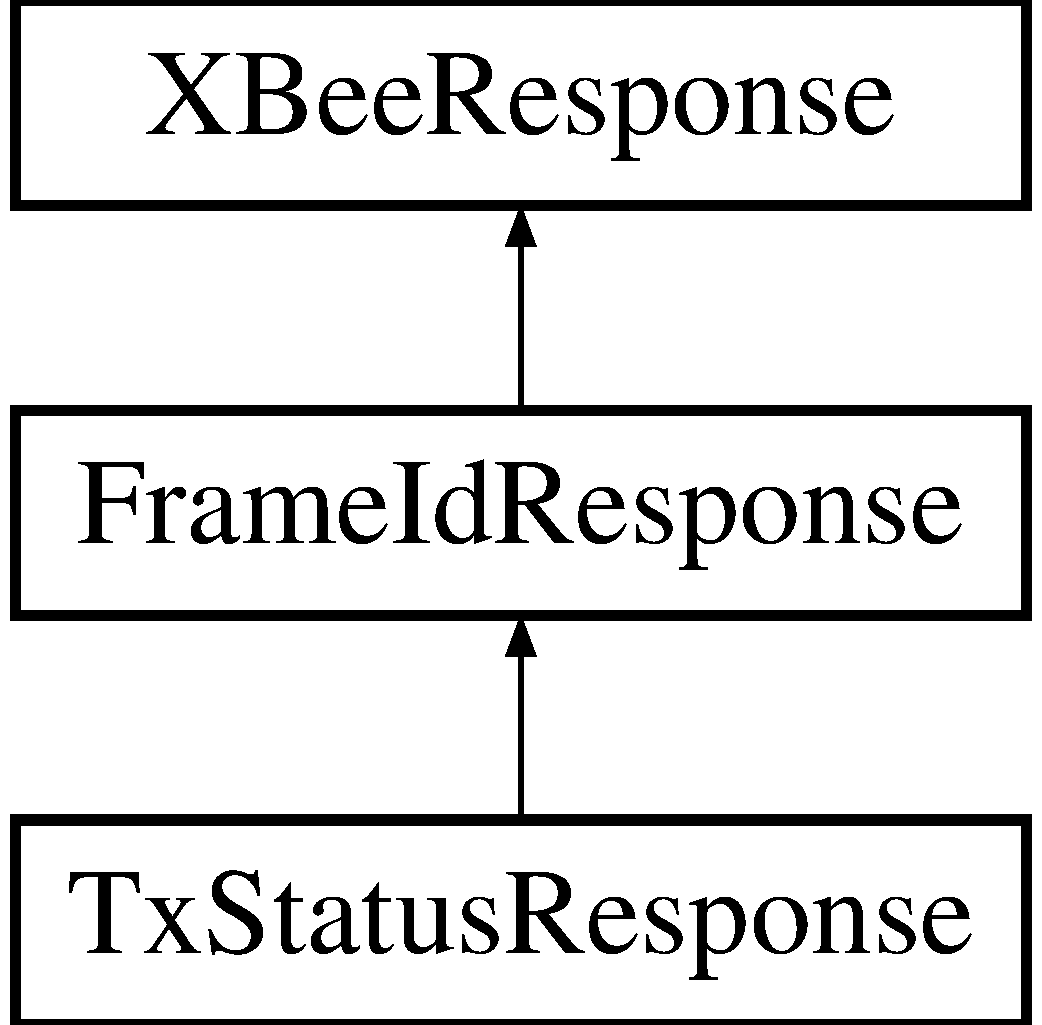
\includegraphics[height=3.000000cm]{classTxStatusResponse}
\end{center}
\end{figure}
\subsection*{\-Public \-Member \-Functions}
\begin{DoxyCompactItemize}
\item 
\hypertarget{classTxStatusResponse_ac6670f7b35b65d9d032c8c4689617569}{uint8\-\_\-t {\bfseries get\-Status} ()}\label{classTxStatusResponse_ac6670f7b35b65d9d032c8c4689617569}

\item 
\hypertarget{classTxStatusResponse_ab5a35099727e48e2a3db12d844881607}{bool {\bfseries is\-Success} ()}\label{classTxStatusResponse_ab5a35099727e48e2a3db12d844881607}

\end{DoxyCompactItemize}


\subsection{\-Detailed \-Description}
\-Represents a \-Series 1 \-T\-X \-Status packet 

\-The documentation for this class was generated from the following files\-:\begin{DoxyCompactItemize}
\item 
\-X\-Bee.\-h\item 
\-X\-Bee.\-cpp\end{DoxyCompactItemize}

\hypertarget{classXBee}{\section{\-X\-Bee \-Class \-Reference}
\label{classXBee}\index{\-X\-Bee@{\-X\-Bee}}
}


{\ttfamily \#include $<$\-X\-Bee.\-h$>$}

\subsection*{\-Public \-Member \-Functions}
\begin{DoxyCompactItemize}
\item 
void \hyperlink{classXBee_a7d788232f44e8b3c10dc686a0299fcc6}{read\-Packet} ()
\item 
bool \hyperlink{classXBee_ae1c9f3b53df50564ab9aca2716792b44}{read\-Packet} (int timeout)
\item 
void \hyperlink{classXBee_a594e2bb2ccb7b3fe7a2278b9324b4083}{read\-Packet\-Until\-Available} ()
\item 
void \hyperlink{classXBee_a847a36fa06c9567496a7ec140cb72586}{begin} (long baud)
\item 
\hypertarget{classXBee_ac88079aa744d36b26a0c6a0add939898}{void {\bfseries get\-Response} (\hyperlink{classXBeeResponse}{\-X\-Bee\-Response} \&response)}\label{classXBee_ac88079aa744d36b26a0c6a0add939898}

\item 
\hyperlink{classXBeeResponse}{\-X\-Bee\-Response} \& \hyperlink{classXBee_a18250def80e8b643aa1ccc15a98937f3}{get\-Response} ()
\item 
void \hyperlink{classXBee_a802387f468be8622941d16739ac848f2}{send} (\hyperlink{classXBeeRequest}{\-X\-Bee\-Request} \&request)
\item 
uint8\-\_\-t \hyperlink{classXBee_a25bd226e41517e8a66a13e531d31438d}{get\-Next\-Frame\-Id} ()
\item 
void \hyperlink{classXBee_a8522ebba19c2751677131b7bb43da6c3}{set\-Serial} (\-Hardware\-Serial \&serial)
\end{DoxyCompactItemize}


\subsection{\-Detailed \-Description}
\-Primary interface for communicating with an \hyperlink{classXBee}{\-X\-Bee} \-Radio. \-This class provides methods for sending and receiving packets with an \hyperlink{classXBee}{\-X\-Bee} radio via the serial port. \-The \hyperlink{classXBee}{\-X\-Bee} radio must be configured in \-A\-P\-I (packet) mode (\-A\-P=2) in order to use this software. 

\-Since this code is designed to run on a microcontroller, with only one thread, you are responsible for reading the data off the serial buffer in a timely manner. \-This involves a call to a variant of read\-Packet(...). \-If your serial port is receiving data faster than you are reading, you can expect to lose packets. \-Arduino only has a 128 byte serial buffer so it can easily overflow if two or more packets arrive without a call to read\-Packet(...) 

\-In order to conserve resources, this class only supports storing one response packet in memory at a time. \-This means that you must fully consume the packet prior to calling read\-Packet(...), because calling read\-Packet(...) overwrites the previous response. 

\-This class creates an array of size \-M\-A\-X\-\_\-\-F\-R\-A\-M\-E\-\_\-\-D\-A\-T\-A\-\_\-\-S\-I\-Z\-E for storing the response packet. \-You may want to adjust this value to conserve memory.

\begin{DoxyAuthor}{\-Author}
\-Andrew \-Rapp 
\end{DoxyAuthor}


\subsection{\-Member \-Function \-Documentation}
\hypertarget{classXBee_a847a36fa06c9567496a7ec140cb72586}{\index{\-X\-Bee@{\-X\-Bee}!begin@{begin}}
\index{begin@{begin}!XBee@{\-X\-Bee}}
\subsubsection[{begin}]{\setlength{\rightskip}{0pt plus 5cm}void {\bf \-X\-Bee\-::begin} (
\begin{DoxyParamCaption}
\item[{long}]{baud}
\end{DoxyParamCaption}
)}}\label{classXBee_a847a36fa06c9567496a7ec140cb72586}
\-Starts the serial connection at the supplied baud rate \hypertarget{classXBee_a25bd226e41517e8a66a13e531d31438d}{\index{\-X\-Bee@{\-X\-Bee}!get\-Next\-Frame\-Id@{get\-Next\-Frame\-Id}}
\index{get\-Next\-Frame\-Id@{get\-Next\-Frame\-Id}!XBee@{\-X\-Bee}}
\subsubsection[{get\-Next\-Frame\-Id}]{\setlength{\rightskip}{0pt plus 5cm}uint8\-\_\-t {\bf \-X\-Bee\-::get\-Next\-Frame\-Id} (
\begin{DoxyParamCaption}
{}
\end{DoxyParamCaption}
)}}\label{classXBee_a25bd226e41517e8a66a13e531d31438d}
\-Returns a sequential frame id between 1 and 255 \hypertarget{classXBee_a18250def80e8b643aa1ccc15a98937f3}{\index{\-X\-Bee@{\-X\-Bee}!get\-Response@{get\-Response}}
\index{get\-Response@{get\-Response}!XBee@{\-X\-Bee}}
\subsubsection[{get\-Response}]{\setlength{\rightskip}{0pt plus 5cm}{\bf \-X\-Bee\-Response} \& \-X\-Bee\-::get\-Response (
\begin{DoxyParamCaption}
{}
\end{DoxyParamCaption}
)}}\label{classXBee_a18250def80e8b643aa1ccc15a98937f3}
\-Returns a reference to the current response \-Note\-: once read\-Packet is called again this response will be overwritten! \hypertarget{classXBee_a7d788232f44e8b3c10dc686a0299fcc6}{\index{\-X\-Bee@{\-X\-Bee}!read\-Packet@{read\-Packet}}
\index{read\-Packet@{read\-Packet}!XBee@{\-X\-Bee}}
\subsubsection[{read\-Packet}]{\setlength{\rightskip}{0pt plus 5cm}void {\bf \-X\-Bee\-::read\-Packet} (
\begin{DoxyParamCaption}
{}
\end{DoxyParamCaption}
)}}\label{classXBee_a7d788232f44e8b3c10dc686a0299fcc6}
\-Reads all available serial bytes until a packet is parsed, an error occurs, or the buffer is empty. \-You may call {\itshape xbee\/}.\hyperlink{classXBee_a18250def80e8b643aa1ccc15a98937f3}{get\-Response()}.is\-Available() after calling this method to determine if a packet is ready, or {\itshape xbee\/}.\hyperlink{classXBee_a18250def80e8b643aa1ccc15a98937f3}{get\-Response()}.is\-Error() to determine if a error occurred. 

\-This method should always return quickly since it does not wait for serial data to arrive. \-You will want to use this method if you are doing other timely stuff in your loop, where a delay would cause problems. \-N\-O\-T\-E\-: calling this method resets the current response, so make sure you first consume the current response \hypertarget{classXBee_ae1c9f3b53df50564ab9aca2716792b44}{\index{\-X\-Bee@{\-X\-Bee}!read\-Packet@{read\-Packet}}
\index{read\-Packet@{read\-Packet}!XBee@{\-X\-Bee}}
\subsubsection[{read\-Packet}]{\setlength{\rightskip}{0pt plus 5cm}bool {\bf \-X\-Bee\-::read\-Packet} (
\begin{DoxyParamCaption}
\item[{int}]{timeout}
\end{DoxyParamCaption}
)}}\label{classXBee_ae1c9f3b53df50564ab9aca2716792b44}
\-Waits a maximum of {\itshape timeout\/} milliseconds for a response packet before timing out; returns true if packet is read. \-Returns false if timeout or error occurs. \hypertarget{classXBee_a594e2bb2ccb7b3fe7a2278b9324b4083}{\index{\-X\-Bee@{\-X\-Bee}!read\-Packet\-Until\-Available@{read\-Packet\-Until\-Available}}
\index{read\-Packet\-Until\-Available@{read\-Packet\-Until\-Available}!XBee@{\-X\-Bee}}
\subsubsection[{read\-Packet\-Until\-Available}]{\setlength{\rightskip}{0pt plus 5cm}void {\bf \-X\-Bee\-::read\-Packet\-Until\-Available} (
\begin{DoxyParamCaption}
{}
\end{DoxyParamCaption}
)}}\label{classXBee_a594e2bb2ccb7b3fe7a2278b9324b4083}
\-Reads until a packet is received or an error occurs. \-Caution\-: use this carefully since if you don't get a response, your \-Arduino code will hang on this call forever!! often it's better to use a timeout\-: \hyperlink{classXBee_ae1c9f3b53df50564ab9aca2716792b44}{read\-Packet(int)} \hypertarget{classXBee_a802387f468be8622941d16739ac848f2}{\index{\-X\-Bee@{\-X\-Bee}!send@{send}}
\index{send@{send}!XBee@{\-X\-Bee}}
\subsubsection[{send}]{\setlength{\rightskip}{0pt plus 5cm}void {\bf \-X\-Bee\-::send} (
\begin{DoxyParamCaption}
\item[{{\bf \-X\-Bee\-Request} \&}]{request}
\end{DoxyParamCaption}
)}}\label{classXBee_a802387f468be8622941d16739ac848f2}
\-Sends a \hyperlink{classXBeeRequest}{\-X\-Bee\-Request} (\-T\-X packet) out the serial port \hypertarget{classXBee_a8522ebba19c2751677131b7bb43da6c3}{\index{\-X\-Bee@{\-X\-Bee}!set\-Serial@{set\-Serial}}
\index{set\-Serial@{set\-Serial}!XBee@{\-X\-Bee}}
\subsubsection[{set\-Serial}]{\setlength{\rightskip}{0pt plus 5cm}void {\bf \-X\-Bee\-::set\-Serial} (
\begin{DoxyParamCaption}
\item[{\-Hardware\-Serial \&}]{serial}
\end{DoxyParamCaption}
)}}\label{classXBee_a8522ebba19c2751677131b7bb43da6c3}
\-Specify the serial port. \-Only relevant for \-Arduinos that support multiple serial ports (e.\-g. \-Mega) 

\-The documentation for this class was generated from the following files\-:\begin{DoxyCompactItemize}
\item 
\-X\-Bee.\-h\item 
\-X\-Bee.\-cpp\end{DoxyCompactItemize}

\hypertarget{classXBeeAddress}{\section{\-X\-Bee\-Address \-Class \-Reference}
\label{classXBeeAddress}\index{\-X\-Bee\-Address@{\-X\-Bee\-Address}}
}
\-Inheritance diagram for \-X\-Bee\-Address\-:\begin{figure}[H]
\begin{center}
\leavevmode
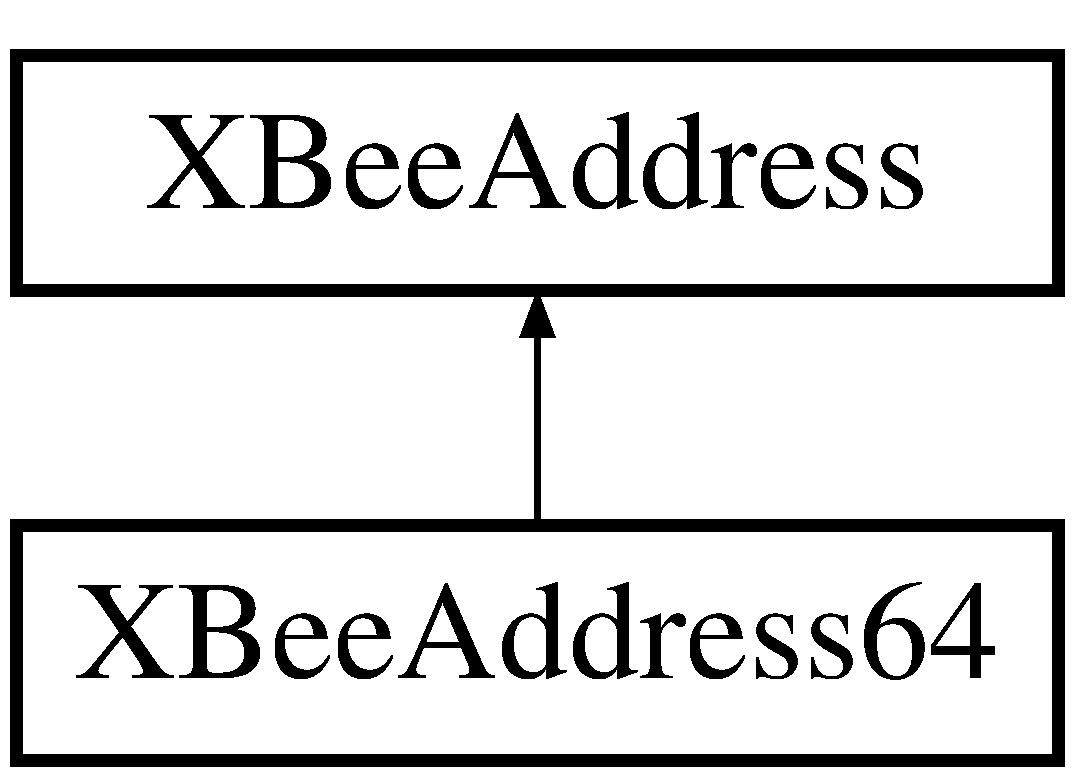
\includegraphics[height=2.000000cm]{classXBeeAddress}
\end{center}
\end{figure}


\-The documentation for this class was generated from the following files\-:\begin{DoxyCompactItemize}
\item 
\-X\-Bee.\-h\item 
\-X\-Bee.\-cpp\end{DoxyCompactItemize}

\hypertarget{classXBeeAddress64}{\section{\-X\-Bee\-Address64 \-Class \-Reference}
\label{classXBeeAddress64}\index{\-X\-Bee\-Address64@{\-X\-Bee\-Address64}}
}


{\ttfamily \#include $<$\-X\-Bee.\-h$>$}

\-Inheritance diagram for \-X\-Bee\-Address64\-:\begin{figure}[H]
\begin{center}
\leavevmode
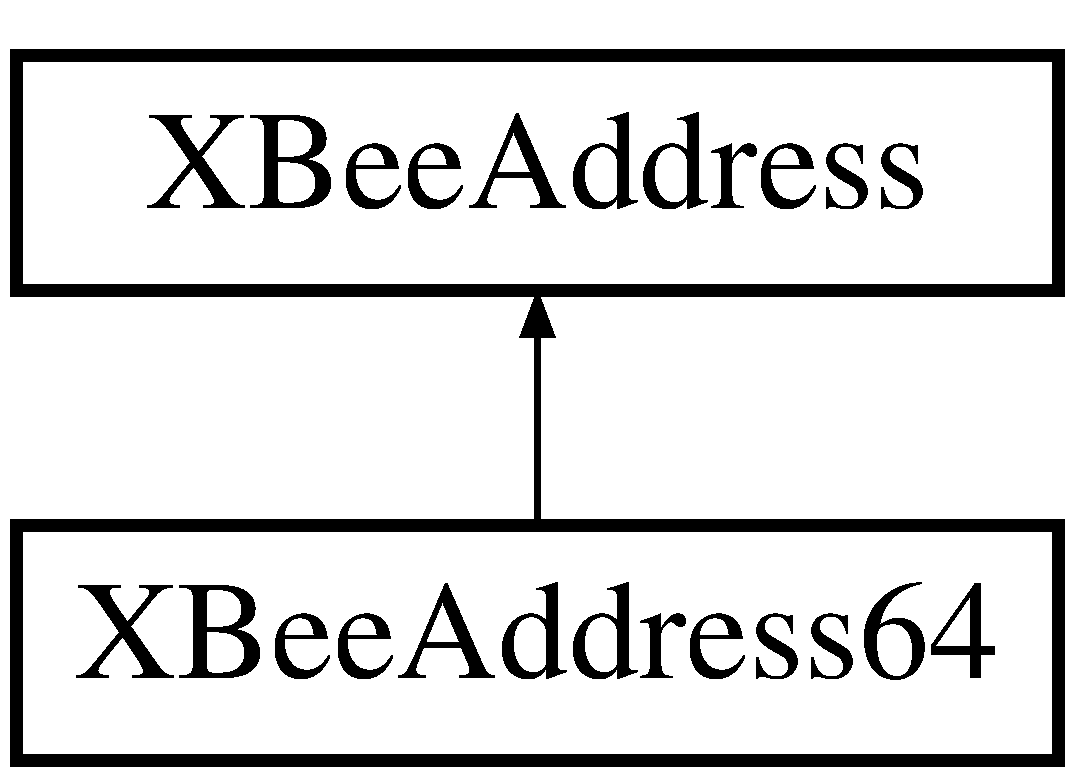
\includegraphics[height=2.000000cm]{classXBeeAddress64}
\end{center}
\end{figure}
\subsection*{\-Public \-Member \-Functions}
\begin{DoxyCompactItemize}
\item 
\hypertarget{classXBeeAddress64_adfa0a20959a1f4255865e8412c668ad9}{{\bfseries \-X\-Bee\-Address64} (uint32\-\_\-t msb, uint32\-\_\-t lsb)}\label{classXBeeAddress64_adfa0a20959a1f4255865e8412c668ad9}

\item 
\hypertarget{classXBeeAddress64_a45b6fd6840c54b9b0c171043bc188010}{uint32\-\_\-t {\bfseries get\-Msb} ()}\label{classXBeeAddress64_a45b6fd6840c54b9b0c171043bc188010}

\item 
\hypertarget{classXBeeAddress64_aafc931f117f53cccbf21d70e9eb31d5c}{uint32\-\_\-t {\bfseries get\-Lsb} ()}\label{classXBeeAddress64_aafc931f117f53cccbf21d70e9eb31d5c}

\item 
\hypertarget{classXBeeAddress64_a35323c4cf8844715d0fc688ef0626352}{void {\bfseries set\-Msb} (uint32\-\_\-t msb)}\label{classXBeeAddress64_a35323c4cf8844715d0fc688ef0626352}

\item 
\hypertarget{classXBeeAddress64_a99a11e8801c87076ec816adeecf087ee}{void {\bfseries set\-Lsb} (uint32\-\_\-t lsb)}\label{classXBeeAddress64_a99a11e8801c87076ec816adeecf087ee}

\end{DoxyCompactItemize}


\subsection{\-Detailed \-Description}
\-Represents a 64-\/bit \hyperlink{classXBee}{\-X\-Bee} \-Address 

\-The documentation for this class was generated from the following files\-:\begin{DoxyCompactItemize}
\item 
\-X\-Bee.\-h\item 
\-X\-Bee.\-cpp\end{DoxyCompactItemize}

\hypertarget{classXBeeRequest}{\section{\-X\-Bee\-Request \-Class \-Reference}
\label{classXBeeRequest}\index{\-X\-Bee\-Request@{\-X\-Bee\-Request}}
}


{\ttfamily \#include $<$\-X\-Bee.\-h$>$}

\-Inheritance diagram for \-X\-Bee\-Request\-:\begin{figure}[H]
\begin{center}
\leavevmode
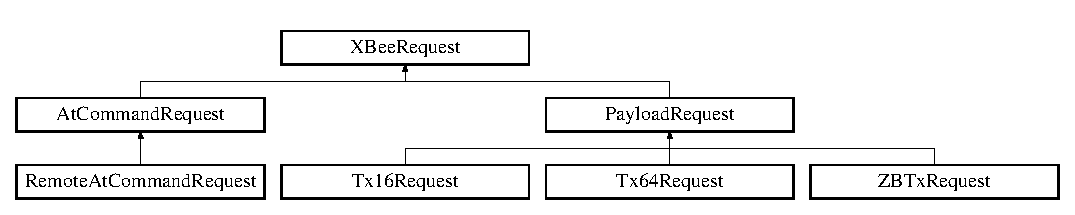
\includegraphics[height=2.441860cm]{classXBeeRequest}
\end{center}
\end{figure}
\subsection*{\-Public \-Member \-Functions}
\begin{DoxyCompactItemize}
\item 
\hyperlink{classXBeeRequest_af80fd559cab746ab8573087cddda71a2}{\-X\-Bee\-Request} (uint8\-\_\-t api\-Id, uint8\-\_\-t frame\-Id)
\item 
void \hyperlink{classXBeeRequest_aed1724c11e710217807c971e40105c86}{set\-Frame\-Id} (uint8\-\_\-t frame\-Id)
\item 
uint8\-\_\-t \hyperlink{classXBeeRequest_a20394c7ea4666224c50bef25cc0cd836}{get\-Frame\-Id} ()
\item 
uint8\-\_\-t \hyperlink{classXBeeRequest_a746d0373c9fb6ed0ff8b7e04f5fb12c9}{get\-Api\-Id} ()
\item 
virtual uint8\-\_\-t \hyperlink{classXBeeRequest_ad5b998cd95a570bdaa4d74c6c8790d94}{get\-Frame\-Data} (uint8\-\_\-t pos)=0
\item 
virtual uint8\-\_\-t \hyperlink{classXBeeRequest_a03b6c558db5836fa7167c0fba7405642}{get\-Frame\-Data\-Length} ()=0
\end{DoxyCompactItemize}
\subsection*{\-Protected \-Member \-Functions}
\begin{DoxyCompactItemize}
\item 
\hypertarget{classXBeeRequest_aee756672e79dbb05358187cb53f61b1a}{void {\bfseries set\-Api\-Id} (uint8\-\_\-t api\-Id)}\label{classXBeeRequest_aee756672e79dbb05358187cb53f61b1a}

\end{DoxyCompactItemize}


\subsection{\-Detailed \-Description}
\-Super class of all \hyperlink{classXBee}{\-X\-Bee} requests (\-T\-X packets) \-Users should never create an instance of this class; instead use an subclass of this class \-It is recommended to reuse \-Subclasses of the class to conserve memory 

\-This class allocates a buffer to 

\subsection{\-Constructor \& \-Destructor \-Documentation}
\hypertarget{classXBeeRequest_af80fd559cab746ab8573087cddda71a2}{\index{\-X\-Bee\-Request@{\-X\-Bee\-Request}!\-X\-Bee\-Request@{\-X\-Bee\-Request}}
\index{\-X\-Bee\-Request@{\-X\-Bee\-Request}!XBeeRequest@{\-X\-Bee\-Request}}
\subsubsection[{\-X\-Bee\-Request}]{\setlength{\rightskip}{0pt plus 5cm}{\bf \-X\-Bee\-Request\-::\-X\-Bee\-Request} (
\begin{DoxyParamCaption}
\item[{uint8\-\_\-t}]{api\-Id, }
\item[{uint8\-\_\-t}]{frame\-Id}
\end{DoxyParamCaption}
)}}\label{classXBeeRequest_af80fd559cab746ab8573087cddda71a2}
\-Constructor \-T\-O\-D\-O make protected 

\subsection{\-Member \-Function \-Documentation}
\hypertarget{classXBeeRequest_a746d0373c9fb6ed0ff8b7e04f5fb12c9}{\index{\-X\-Bee\-Request@{\-X\-Bee\-Request}!get\-Api\-Id@{get\-Api\-Id}}
\index{get\-Api\-Id@{get\-Api\-Id}!XBeeRequest@{\-X\-Bee\-Request}}
\subsubsection[{get\-Api\-Id}]{\setlength{\rightskip}{0pt plus 5cm}uint8\-\_\-t {\bf \-X\-Bee\-Request\-::get\-Api\-Id} (
\begin{DoxyParamCaption}
{}
\end{DoxyParamCaption}
)}}\label{classXBeeRequest_a746d0373c9fb6ed0ff8b7e04f5fb12c9}
\-Returns the \-A\-P\-I id \hypertarget{classXBeeRequest_ad5b998cd95a570bdaa4d74c6c8790d94}{\index{\-X\-Bee\-Request@{\-X\-Bee\-Request}!get\-Frame\-Data@{get\-Frame\-Data}}
\index{get\-Frame\-Data@{get\-Frame\-Data}!XBeeRequest@{\-X\-Bee\-Request}}
\subsubsection[{get\-Frame\-Data}]{\setlength{\rightskip}{0pt plus 5cm}virtual uint8\-\_\-t {\bf \-X\-Bee\-Request\-::get\-Frame\-Data} (
\begin{DoxyParamCaption}
\item[{uint8\-\_\-t}]{pos}
\end{DoxyParamCaption}
)\hspace{0.3cm}{\ttfamily  \mbox{[}pure virtual\mbox{]}}}}\label{classXBeeRequest_ad5b998cd95a570bdaa4d74c6c8790d94}
\-Starting after the frame id (pos = 0) and up to but not including the checksum \-Note\-: \-Unlike \-Digi's definition of the frame data, this does not start with the \-A\-P\-I \-I\-D. \-The reason for this is the \-A\-P\-I \-I\-D and \-Frame \-I\-D are common to all requests, whereas my definition of frame data is only the \-A\-P\-I specific data. 

\-Implemented in \hyperlink{classRemoteAtCommandRequest_a0e576cf564ebd5a82cb2ed05239a856a}{\-Remote\-At\-Command\-Request}, \hyperlink{classAtCommandRequest_aa4fc8f0c8404172cd5532f3d8e5564f2}{\-At\-Command\-Request}, \hyperlink{classZBTxRequest_ac81e09dfbf7aefbdf7f8b4838b643c5c}{\-Z\-B\-Tx\-Request}, \hyperlink{classTx64Request_afe3662433da85acd21f8a3d90844a084}{\-Tx64\-Request}, and \hyperlink{classTx16Request_af5ffbc2164e766d96f54c723996fd389}{\-Tx16\-Request}.

\hypertarget{classXBeeRequest_a03b6c558db5836fa7167c0fba7405642}{\index{\-X\-Bee\-Request@{\-X\-Bee\-Request}!get\-Frame\-Data\-Length@{get\-Frame\-Data\-Length}}
\index{get\-Frame\-Data\-Length@{get\-Frame\-Data\-Length}!XBeeRequest@{\-X\-Bee\-Request}}
\subsubsection[{get\-Frame\-Data\-Length}]{\setlength{\rightskip}{0pt plus 5cm}virtual uint8\-\_\-t {\bf \-X\-Bee\-Request\-::get\-Frame\-Data\-Length} (
\begin{DoxyParamCaption}
{}
\end{DoxyParamCaption}
)\hspace{0.3cm}{\ttfamily  \mbox{[}pure virtual\mbox{]}}}}\label{classXBeeRequest_a03b6c558db5836fa7167c0fba7405642}
\-Returns the size of the api frame (not including frame id or api id or checksum). 

\-Implemented in \hyperlink{classRemoteAtCommandRequest_a1d78334a8924b0a0e06de6ef3a09c24f}{\-Remote\-At\-Command\-Request}, \hyperlink{classAtCommandRequest_aad12b8357e63fca9e95b6731a4bfda0d}{\-At\-Command\-Request}, \hyperlink{classZBTxRequest_a8e6914c1f556981a0f863c57c57d053b}{\-Z\-B\-Tx\-Request}, \hyperlink{classTx64Request_afadc1e07718a62d6c5a75a4bb07dfaae}{\-Tx64\-Request}, and \hyperlink{classTx16Request_a9a1ddfb380e72ecc09a024c6de6cdf8e}{\-Tx16\-Request}.

\hypertarget{classXBeeRequest_a20394c7ea4666224c50bef25cc0cd836}{\index{\-X\-Bee\-Request@{\-X\-Bee\-Request}!get\-Frame\-Id@{get\-Frame\-Id}}
\index{get\-Frame\-Id@{get\-Frame\-Id}!XBeeRequest@{\-X\-Bee\-Request}}
\subsubsection[{get\-Frame\-Id}]{\setlength{\rightskip}{0pt plus 5cm}uint8\-\_\-t {\bf \-X\-Bee\-Request\-::get\-Frame\-Id} (
\begin{DoxyParamCaption}
{}
\end{DoxyParamCaption}
)}}\label{classXBeeRequest_a20394c7ea4666224c50bef25cc0cd836}
\-Returns the frame id \hypertarget{classXBeeRequest_aed1724c11e710217807c971e40105c86}{\index{\-X\-Bee\-Request@{\-X\-Bee\-Request}!set\-Frame\-Id@{set\-Frame\-Id}}
\index{set\-Frame\-Id@{set\-Frame\-Id}!XBeeRequest@{\-X\-Bee\-Request}}
\subsubsection[{set\-Frame\-Id}]{\setlength{\rightskip}{0pt plus 5cm}void {\bf \-X\-Bee\-Request\-::set\-Frame\-Id} (
\begin{DoxyParamCaption}
\item[{uint8\-\_\-t}]{frame\-Id}
\end{DoxyParamCaption}
)}}\label{classXBeeRequest_aed1724c11e710217807c971e40105c86}
\-Sets the frame id. \-Must be between 1 and 255 inclusive to get a \-T\-X status response. 

\-The documentation for this class was generated from the following files\-:\begin{DoxyCompactItemize}
\item 
\-X\-Bee.\-h\item 
\-X\-Bee.\-cpp\end{DoxyCompactItemize}

\hypertarget{classXBeeResponse}{\section{\-X\-Bee\-Response \-Class \-Reference}
\label{classXBeeResponse}\index{\-X\-Bee\-Response@{\-X\-Bee\-Response}}
}


{\ttfamily \#include $<$\-X\-Bee.\-h$>$}

\-Inheritance diagram for \-X\-Bee\-Response\-:\begin{figure}[H]
\begin{center}
\leavevmode
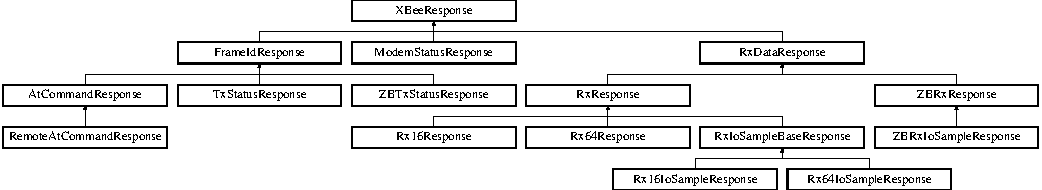
\includegraphics[height=2.550091cm]{classXBeeResponse}
\end{center}
\end{figure}
\subsection*{\-Public \-Member \-Functions}
\begin{DoxyCompactItemize}
\item 
\hyperlink{classXBeeResponse_a03a6ea7651a40062c22ca0a37fbf512f}{\-X\-Bee\-Response} ()
\item 
uint8\-\_\-t \hyperlink{classXBeeResponse_a4a9677e3b39054119fa278d1ad52130a}{get\-Api\-Id} ()
\item 
\hypertarget{classXBeeResponse_a68177a43b06ba96b901759a491aae073}{void {\bfseries set\-Api\-Id} (uint8\-\_\-t api\-Id)}\label{classXBeeResponse_a68177a43b06ba96b901759a491aae073}

\item 
uint8\-\_\-t \hyperlink{classXBeeResponse_aae9f85f70cbcb92cfcc278295a947952}{get\-Msb\-Length} ()
\item 
\hypertarget{classXBeeResponse_a9aa50d1df15ff44b24ffb299854dba74}{void {\bfseries set\-Msb\-Length} (uint8\-\_\-t msb\-Length)}\label{classXBeeResponse_a9aa50d1df15ff44b24ffb299854dba74}

\item 
uint8\-\_\-t \hyperlink{classXBeeResponse_acb1b40edafa22461776b75bd5d7caadf}{get\-Lsb\-Length} ()
\item 
\hypertarget{classXBeeResponse_a796fd65123825128715e51e6300e9e58}{void {\bfseries set\-Lsb\-Length} (uint8\-\_\-t lsb\-Length)}\label{classXBeeResponse_a796fd65123825128715e51e6300e9e58}

\item 
uint8\-\_\-t \hyperlink{classXBeeResponse_aa8f34253bb77196366ea8ac9bc318734}{get\-Checksum} ()
\item 
\hypertarget{classXBeeResponse_af69cfaa7c99e6aab2236c8f11ab07940}{void {\bfseries set\-Checksum} (uint8\-\_\-t checksum)}\label{classXBeeResponse_af69cfaa7c99e6aab2236c8f11ab07940}

\item 
uint8\-\_\-t \hyperlink{classXBeeResponse_a6205be340c4f0397a68dadbdca36a091}{get\-Frame\-Data\-Length} ()
\item 
\hypertarget{classXBeeResponse_a13788c12c5201769a304880335749b69}{void {\bfseries set\-Frame\-Data} (uint8\-\_\-t $\ast$frame\-Data\-Ptr)}\label{classXBeeResponse_a13788c12c5201769a304880335749b69}

\item 
uint8\-\_\-t $\ast$ \hyperlink{classXBeeResponse_ad958f0b5200138545bdd762111299a94}{get\-Frame\-Data} ()
\item 
\hypertarget{classXBeeResponse_ad2419bab7589e82b5358482c1abbe87c}{void {\bfseries set\-Frame\-Length} (uint8\-\_\-t frame\-Length)}\label{classXBeeResponse_ad2419bab7589e82b5358482c1abbe87c}

\item 
uint16\-\_\-t \hyperlink{classXBeeResponse_a26a7c8baad9cc0322a38db997685d889}{get\-Packet\-Length} ()
\item 
void \hyperlink{classXBeeResponse_aa08a73f576fc7ce2f7fa154342c01fba}{reset} ()
\item 
void \hyperlink{classXBeeResponse_af084604e35462783ecd293ffc090d6dc}{init} ()
\item 
void \hyperlink{classXBeeResponse_a1353f14b87b9cbdc1f8001fb8c5e9d35}{get\-Z\-B\-Tx\-Status\-Response} (\hyperlink{classXBeeResponse}{\-X\-Bee\-Response} \&response)
\item 
void \hyperlink{classXBeeResponse_a4c0edfc6be81349237956531a006d3ab}{get\-Z\-B\-Rx\-Response} (\hyperlink{classXBeeResponse}{\-X\-Bee\-Response} \&response)
\item 
void \hyperlink{classXBeeResponse_a0c1f8d66b1b276fd6d482c589d5cda3d}{get\-Z\-B\-Rx\-Io\-Sample\-Response} (\hyperlink{classXBeeResponse}{\-X\-Bee\-Response} \&response)
\item 
void \hyperlink{classXBeeResponse_a2fd9882d767d48e679a7595b780c2a2d}{get\-Tx\-Status\-Response} (\hyperlink{classXBeeResponse}{\-X\-Bee\-Response} \&response)
\item 
void \hyperlink{classXBeeResponse_ab85f25eac3e57d665e2189d84cb5d2e3}{get\-Rx16\-Response} (\hyperlink{classXBeeResponse}{\-X\-Bee\-Response} \&response)
\item 
void \hyperlink{classXBeeResponse_a72e5b863c14a9ec0a4f1cdeba5f24e58}{get\-Rx64\-Response} (\hyperlink{classXBeeResponse}{\-X\-Bee\-Response} \&response)
\item 
void \hyperlink{classXBeeResponse_ae84d38e3759ebf8b23d256b207e5761d}{get\-Rx16\-Io\-Sample\-Response} (\hyperlink{classXBeeResponse}{\-X\-Bee\-Response} \&response)
\item 
void \hyperlink{classXBeeResponse_ae298de16ed0dce349154ae87f8b93d77}{get\-Rx64\-Io\-Sample\-Response} (\hyperlink{classXBeeResponse}{\-X\-Bee\-Response} \&response)
\item 
void \hyperlink{classXBeeResponse_a5177bb036ccaa6ea30d73541a3e7d414}{get\-At\-Command\-Response} (\hyperlink{classXBeeResponse}{\-X\-Bee\-Response} \&responses)
\item 
void \hyperlink{classXBeeResponse_af359dab94c57006a0fb4b58986744c04}{get\-Remote\-At\-Command\-Response} (\hyperlink{classXBeeResponse}{\-X\-Bee\-Response} \&response)
\item 
void \hyperlink{classXBeeResponse_ad93317521b52825c32b43d34a0f189d1}{get\-Modem\-Status\-Response} (\hyperlink{classXBeeResponse}{\-X\-Bee\-Response} \&response)
\item 
bool \hyperlink{classXBeeResponse_ab60b2cc9e32fa88dee132f410cc8331d}{is\-Available} ()
\item 
\hypertarget{classXBeeResponse_a1814031d09ed316de9f983bd367f3ae4}{void {\bfseries set\-Available} (bool complete)}\label{classXBeeResponse_a1814031d09ed316de9f983bd367f3ae4}

\item 
bool \hyperlink{classXBeeResponse_a68cbc45004ff4314161b0fb1cc579b9b}{is\-Error} ()
\item 
uint8\-\_\-t \hyperlink{classXBeeResponse_a2895438378d2738e3efe74b1c838170b}{get\-Error\-Code} ()
\item 
\hypertarget{classXBeeResponse_a95749b78c9807e8f403abf1620ab29c1}{void {\bfseries set\-Error\-Code} (uint8\-\_\-t error\-Code)}\label{classXBeeResponse_a95749b78c9807e8f403abf1620ab29c1}

\end{DoxyCompactItemize}
\subsection*{\-Protected \-Attributes}
\begin{DoxyCompactItemize}
\item 
\hypertarget{classXBeeResponse_af62a61818a476f4815d93f9c3485e6e7}{uint8\-\_\-t $\ast$ {\bfseries \-\_\-frame\-Data\-Ptr}}\label{classXBeeResponse_af62a61818a476f4815d93f9c3485e6e7}

\end{DoxyCompactItemize}


\subsection{\-Detailed \-Description}
\-The super class of all \hyperlink{classXBee}{\-X\-Bee} responses (\-R\-X packets) \-Users should never attempt to create an instance of this class; instead create an instance of a subclass \-It is recommend to reuse subclasses to conserve memory 

\subsection{\-Constructor \& \-Destructor \-Documentation}
\hypertarget{classXBeeResponse_a03a6ea7651a40062c22ca0a37fbf512f}{\index{\-X\-Bee\-Response@{\-X\-Bee\-Response}!\-X\-Bee\-Response@{\-X\-Bee\-Response}}
\index{\-X\-Bee\-Response@{\-X\-Bee\-Response}!XBeeResponse@{\-X\-Bee\-Response}}
\subsubsection[{\-X\-Bee\-Response}]{\setlength{\rightskip}{0pt plus 5cm}{\bf \-X\-Bee\-Response\-::\-X\-Bee\-Response} (
\begin{DoxyParamCaption}
{}
\end{DoxyParamCaption}
)}}\label{classXBeeResponse_a03a6ea7651a40062c22ca0a37fbf512f}
\-Default constructor

\-Copyright (c) 2009 \-Andrew \-Rapp. \-All rights reserved.

\-This file is part of \-X\-Bee-\/\-Arduino.

\-X\-Bee-\/\-Arduino is free software\-: you can redistribute it and/or modify it under the terms of the \-G\-N\-U \-General \-Public \-License as published by the \-Free \-Software \-Foundation, either version 3 of the \-License, or (at your option) any later version.

\-X\-Bee-\/\-Arduino is distributed in the hope that it will be useful, but \-W\-I\-T\-H\-O\-U\-T \-A\-N\-Y \-W\-A\-R\-R\-A\-N\-T\-Y; without even the implied warranty of \-M\-E\-R\-C\-H\-A\-N\-T\-A\-B\-I\-L\-I\-T\-Y or \-F\-I\-T\-N\-E\-S\-S \-F\-O\-R \-A \-P\-A\-R\-T\-I\-C\-U\-L\-A\-R \-P\-U\-R\-P\-O\-S\-E. \-See the \-G\-N\-U \-General \-Public \-License for more details.

\-You should have received a copy of the \-G\-N\-U \-General \-Public \-License along with \-X\-Bee-\/\-Arduino. \-If not, see $<$\href{http://www.gnu.org/licenses/}{\tt http\-://www.\-gnu.\-org/licenses/}$>$. 

\subsection{\-Member \-Function \-Documentation}
\hypertarget{classXBeeResponse_a4a9677e3b39054119fa278d1ad52130a}{\index{\-X\-Bee\-Response@{\-X\-Bee\-Response}!get\-Api\-Id@{get\-Api\-Id}}
\index{get\-Api\-Id@{get\-Api\-Id}!XBeeResponse@{\-X\-Bee\-Response}}
\subsubsection[{get\-Api\-Id}]{\setlength{\rightskip}{0pt plus 5cm}uint8\-\_\-t {\bf \-X\-Bee\-Response\-::get\-Api\-Id} (
\begin{DoxyParamCaption}
{}
\end{DoxyParamCaption}
)}}\label{classXBeeResponse_a4a9677e3b39054119fa278d1ad52130a}
\-Returns \-Api \-Id of the response \hypertarget{classXBeeResponse_a5177bb036ccaa6ea30d73541a3e7d414}{\index{\-X\-Bee\-Response@{\-X\-Bee\-Response}!get\-At\-Command\-Response@{get\-At\-Command\-Response}}
\index{get\-At\-Command\-Response@{get\-At\-Command\-Response}!XBeeResponse@{\-X\-Bee\-Response}}
\subsubsection[{get\-At\-Command\-Response}]{\setlength{\rightskip}{0pt plus 5cm}void {\bf \-X\-Bee\-Response\-::get\-At\-Command\-Response} (
\begin{DoxyParamCaption}
\item[{{\bf \-X\-Bee\-Response} \&}]{responses}
\end{DoxyParamCaption}
)}}\label{classXBeeResponse_a5177bb036ccaa6ea30d73541a3e7d414}
\-Call with instance of \hyperlink{classAtCommandResponse}{\-At\-Command\-Response} only if \hyperlink{classXBeeResponse_a4a9677e3b39054119fa278d1ad52130a}{get\-Api\-Id()} == \-A\-T\-\_\-\-C\-O\-M\-M\-A\-N\-D\-\_\-\-R\-E\-S\-P\-O\-N\-S\-E \hypertarget{classXBeeResponse_aa8f34253bb77196366ea8ac9bc318734}{\index{\-X\-Bee\-Response@{\-X\-Bee\-Response}!get\-Checksum@{get\-Checksum}}
\index{get\-Checksum@{get\-Checksum}!XBeeResponse@{\-X\-Bee\-Response}}
\subsubsection[{get\-Checksum}]{\setlength{\rightskip}{0pt plus 5cm}uint8\-\_\-t {\bf \-X\-Bee\-Response\-::get\-Checksum} (
\begin{DoxyParamCaption}
{}
\end{DoxyParamCaption}
)}}\label{classXBeeResponse_aa8f34253bb77196366ea8ac9bc318734}
\-Returns the packet checksum \hypertarget{classXBeeResponse_a2895438378d2738e3efe74b1c838170b}{\index{\-X\-Bee\-Response@{\-X\-Bee\-Response}!get\-Error\-Code@{get\-Error\-Code}}
\index{get\-Error\-Code@{get\-Error\-Code}!XBeeResponse@{\-X\-Bee\-Response}}
\subsubsection[{get\-Error\-Code}]{\setlength{\rightskip}{0pt plus 5cm}uint8\-\_\-t {\bf \-X\-Bee\-Response\-::get\-Error\-Code} (
\begin{DoxyParamCaption}
{}
\end{DoxyParamCaption}
)}}\label{classXBeeResponse_a2895438378d2738e3efe74b1c838170b}
\-Returns an error code, or zero, if successful. \-Error codes include\-: \-C\-H\-E\-C\-K\-S\-U\-M\-\_\-\-F\-A\-I\-L\-U\-R\-E, \-P\-A\-C\-K\-E\-T\-\_\-\-E\-X\-C\-E\-E\-D\-S\-\_\-\-B\-Y\-T\-E\-\_\-\-A\-R\-R\-A\-Y\-\_\-\-L\-E\-N\-G\-T\-H, \-U\-N\-E\-X\-P\-E\-C\-T\-E\-D\-\_\-\-S\-T\-A\-R\-T\-\_\-\-B\-Y\-T\-E \hypertarget{classXBeeResponse_ad958f0b5200138545bdd762111299a94}{\index{\-X\-Bee\-Response@{\-X\-Bee\-Response}!get\-Frame\-Data@{get\-Frame\-Data}}
\index{get\-Frame\-Data@{get\-Frame\-Data}!XBeeResponse@{\-X\-Bee\-Response}}
\subsubsection[{get\-Frame\-Data}]{\setlength{\rightskip}{0pt plus 5cm}uint8\-\_\-t $\ast$ {\bf \-X\-Bee\-Response\-::get\-Frame\-Data} (
\begin{DoxyParamCaption}
{}
\end{DoxyParamCaption}
)}}\label{classXBeeResponse_ad958f0b5200138545bdd762111299a94}
\-Returns the buffer that contains the response. \-Starts with byte that follows \-A\-P\-I \-I\-D and includes all bytes prior to the checksum \-Length is specified by \hyperlink{classXBeeResponse_a6205be340c4f0397a68dadbdca36a091}{get\-Frame\-Data\-Length()} \-Note\-: \-Unlike \-Digi's definition of the frame data, this does not start with the \-A\-P\-I \-I\-D.. \-The reason for this is all responses include an \-A\-P\-I \-I\-D, whereas my frame data includes only the \-A\-P\-I specific data. \hypertarget{classXBeeResponse_a6205be340c4f0397a68dadbdca36a091}{\index{\-X\-Bee\-Response@{\-X\-Bee\-Response}!get\-Frame\-Data\-Length@{get\-Frame\-Data\-Length}}
\index{get\-Frame\-Data\-Length@{get\-Frame\-Data\-Length}!XBeeResponse@{\-X\-Bee\-Response}}
\subsubsection[{get\-Frame\-Data\-Length}]{\setlength{\rightskip}{0pt plus 5cm}uint8\-\_\-t {\bf \-X\-Bee\-Response\-::get\-Frame\-Data\-Length} (
\begin{DoxyParamCaption}
{}
\end{DoxyParamCaption}
)}}\label{classXBeeResponse_a6205be340c4f0397a68dadbdca36a091}
\-Returns the length of the frame data\-: all bytes after the api id, and prior to the checksum \-Note up to release 0.\-1.\-2, this was incorrectly including the checksum in the length. \hypertarget{classXBeeResponse_acb1b40edafa22461776b75bd5d7caadf}{\index{\-X\-Bee\-Response@{\-X\-Bee\-Response}!get\-Lsb\-Length@{get\-Lsb\-Length}}
\index{get\-Lsb\-Length@{get\-Lsb\-Length}!XBeeResponse@{\-X\-Bee\-Response}}
\subsubsection[{get\-Lsb\-Length}]{\setlength{\rightskip}{0pt plus 5cm}uint8\-\_\-t {\bf \-X\-Bee\-Response\-::get\-Lsb\-Length} (
\begin{DoxyParamCaption}
{}
\end{DoxyParamCaption}
)}}\label{classXBeeResponse_acb1b40edafa22461776b75bd5d7caadf}
\-Returns the \-L\-S\-B length of the packet \hypertarget{classXBeeResponse_ad93317521b52825c32b43d34a0f189d1}{\index{\-X\-Bee\-Response@{\-X\-Bee\-Response}!get\-Modem\-Status\-Response@{get\-Modem\-Status\-Response}}
\index{get\-Modem\-Status\-Response@{get\-Modem\-Status\-Response}!XBeeResponse@{\-X\-Bee\-Response}}
\subsubsection[{get\-Modem\-Status\-Response}]{\setlength{\rightskip}{0pt plus 5cm}void {\bf \-X\-Bee\-Response\-::get\-Modem\-Status\-Response} (
\begin{DoxyParamCaption}
\item[{{\bf \-X\-Bee\-Response} \&}]{response}
\end{DoxyParamCaption}
)}}\label{classXBeeResponse_ad93317521b52825c32b43d34a0f189d1}
\-Call with instance of \hyperlink{classModemStatusResponse}{\-Modem\-Status\-Response} only if \hyperlink{classXBeeResponse_a4a9677e3b39054119fa278d1ad52130a}{get\-Api\-Id()} == \-M\-O\-D\-E\-M\-\_\-\-S\-T\-A\-T\-U\-S\-\_\-\-R\-E\-S\-P\-O\-N\-S\-E \hypertarget{classXBeeResponse_aae9f85f70cbcb92cfcc278295a947952}{\index{\-X\-Bee\-Response@{\-X\-Bee\-Response}!get\-Msb\-Length@{get\-Msb\-Length}}
\index{get\-Msb\-Length@{get\-Msb\-Length}!XBeeResponse@{\-X\-Bee\-Response}}
\subsubsection[{get\-Msb\-Length}]{\setlength{\rightskip}{0pt plus 5cm}uint8\-\_\-t {\bf \-X\-Bee\-Response\-::get\-Msb\-Length} (
\begin{DoxyParamCaption}
{}
\end{DoxyParamCaption}
)}}\label{classXBeeResponse_aae9f85f70cbcb92cfcc278295a947952}
\-Returns the \-M\-S\-B length of the packet \hypertarget{classXBeeResponse_a26a7c8baad9cc0322a38db997685d889}{\index{\-X\-Bee\-Response@{\-X\-Bee\-Response}!get\-Packet\-Length@{get\-Packet\-Length}}
\index{get\-Packet\-Length@{get\-Packet\-Length}!XBeeResponse@{\-X\-Bee\-Response}}
\subsubsection[{get\-Packet\-Length}]{\setlength{\rightskip}{0pt plus 5cm}uint16\-\_\-t {\bf \-X\-Bee\-Response\-::get\-Packet\-Length} (
\begin{DoxyParamCaption}
{}
\end{DoxyParamCaption}
)}}\label{classXBeeResponse_a26a7c8baad9cc0322a38db997685d889}
\-Returns the length of the packet \hypertarget{classXBeeResponse_af359dab94c57006a0fb4b58986744c04}{\index{\-X\-Bee\-Response@{\-X\-Bee\-Response}!get\-Remote\-At\-Command\-Response@{get\-Remote\-At\-Command\-Response}}
\index{get\-Remote\-At\-Command\-Response@{get\-Remote\-At\-Command\-Response}!XBeeResponse@{\-X\-Bee\-Response}}
\subsubsection[{get\-Remote\-At\-Command\-Response}]{\setlength{\rightskip}{0pt plus 5cm}void {\bf \-X\-Bee\-Response\-::get\-Remote\-At\-Command\-Response} (
\begin{DoxyParamCaption}
\item[{{\bf \-X\-Bee\-Response} \&}]{response}
\end{DoxyParamCaption}
)}}\label{classXBeeResponse_af359dab94c57006a0fb4b58986744c04}
\-Call with instance of \hyperlink{classRemoteAtCommandResponse}{\-Remote\-At\-Command\-Response} only if \hyperlink{classXBeeResponse_a4a9677e3b39054119fa278d1ad52130a}{get\-Api\-Id()} == \-R\-E\-M\-O\-T\-E\-\_\-\-A\-T\-\_\-\-C\-O\-M\-M\-A\-N\-D\-\_\-\-R\-E\-S\-P\-O\-N\-S\-E \hypertarget{classXBeeResponse_ae84d38e3759ebf8b23d256b207e5761d}{\index{\-X\-Bee\-Response@{\-X\-Bee\-Response}!get\-Rx16\-Io\-Sample\-Response@{get\-Rx16\-Io\-Sample\-Response}}
\index{get\-Rx16\-Io\-Sample\-Response@{get\-Rx16\-Io\-Sample\-Response}!XBeeResponse@{\-X\-Bee\-Response}}
\subsubsection[{get\-Rx16\-Io\-Sample\-Response}]{\setlength{\rightskip}{0pt plus 5cm}void {\bf \-X\-Bee\-Response\-::get\-Rx16\-Io\-Sample\-Response} (
\begin{DoxyParamCaption}
\item[{{\bf \-X\-Bee\-Response} \&}]{response}
\end{DoxyParamCaption}
)}}\label{classXBeeResponse_ae84d38e3759ebf8b23d256b207e5761d}
\-Call with instance of \hyperlink{classRx16IoSampleResponse}{\-Rx16\-Io\-Sample\-Response} only if \hyperlink{classXBeeResponse_a4a9677e3b39054119fa278d1ad52130a}{get\-Api\-Id()} == \-R\-X\-\_\-16\-\_\-\-I\-O\-\_\-\-R\-E\-S\-P\-O\-N\-S\-E \hypertarget{classXBeeResponse_ab85f25eac3e57d665e2189d84cb5d2e3}{\index{\-X\-Bee\-Response@{\-X\-Bee\-Response}!get\-Rx16\-Response@{get\-Rx16\-Response}}
\index{get\-Rx16\-Response@{get\-Rx16\-Response}!XBeeResponse@{\-X\-Bee\-Response}}
\subsubsection[{get\-Rx16\-Response}]{\setlength{\rightskip}{0pt plus 5cm}void {\bf \-X\-Bee\-Response\-::get\-Rx16\-Response} (
\begin{DoxyParamCaption}
\item[{{\bf \-X\-Bee\-Response} \&}]{response}
\end{DoxyParamCaption}
)}}\label{classXBeeResponse_ab85f25eac3e57d665e2189d84cb5d2e3}
\-Call with instance of \hyperlink{classRx16Response}{\-Rx16\-Response} only if \hyperlink{classXBeeResponse_a4a9677e3b39054119fa278d1ad52130a}{get\-Api\-Id()} == \-R\-X\-\_\-16\-\_\-\-R\-E\-S\-P\-O\-N\-S\-E \hypertarget{classXBeeResponse_ae298de16ed0dce349154ae87f8b93d77}{\index{\-X\-Bee\-Response@{\-X\-Bee\-Response}!get\-Rx64\-Io\-Sample\-Response@{get\-Rx64\-Io\-Sample\-Response}}
\index{get\-Rx64\-Io\-Sample\-Response@{get\-Rx64\-Io\-Sample\-Response}!XBeeResponse@{\-X\-Bee\-Response}}
\subsubsection[{get\-Rx64\-Io\-Sample\-Response}]{\setlength{\rightskip}{0pt plus 5cm}void {\bf \-X\-Bee\-Response\-::get\-Rx64\-Io\-Sample\-Response} (
\begin{DoxyParamCaption}
\item[{{\bf \-X\-Bee\-Response} \&}]{response}
\end{DoxyParamCaption}
)}}\label{classXBeeResponse_ae298de16ed0dce349154ae87f8b93d77}
\-Call with instance of \hyperlink{classRx64IoSampleResponse}{\-Rx64\-Io\-Sample\-Response} only if \hyperlink{classXBeeResponse_a4a9677e3b39054119fa278d1ad52130a}{get\-Api\-Id()} == \-R\-X\-\_\-64\-\_\-\-I\-O\-\_\-\-R\-E\-S\-P\-O\-N\-S\-E \hypertarget{classXBeeResponse_a72e5b863c14a9ec0a4f1cdeba5f24e58}{\index{\-X\-Bee\-Response@{\-X\-Bee\-Response}!get\-Rx64\-Response@{get\-Rx64\-Response}}
\index{get\-Rx64\-Response@{get\-Rx64\-Response}!XBeeResponse@{\-X\-Bee\-Response}}
\subsubsection[{get\-Rx64\-Response}]{\setlength{\rightskip}{0pt plus 5cm}void {\bf \-X\-Bee\-Response\-::get\-Rx64\-Response} (
\begin{DoxyParamCaption}
\item[{{\bf \-X\-Bee\-Response} \&}]{response}
\end{DoxyParamCaption}
)}}\label{classXBeeResponse_a72e5b863c14a9ec0a4f1cdeba5f24e58}
\-Call with instance of \hyperlink{classRx64Response}{\-Rx64\-Response} only if \hyperlink{classXBeeResponse_a4a9677e3b39054119fa278d1ad52130a}{get\-Api\-Id()} == \-R\-X\-\_\-64\-\_\-\-R\-E\-S\-P\-O\-N\-S\-E \hypertarget{classXBeeResponse_a2fd9882d767d48e679a7595b780c2a2d}{\index{\-X\-Bee\-Response@{\-X\-Bee\-Response}!get\-Tx\-Status\-Response@{get\-Tx\-Status\-Response}}
\index{get\-Tx\-Status\-Response@{get\-Tx\-Status\-Response}!XBeeResponse@{\-X\-Bee\-Response}}
\subsubsection[{get\-Tx\-Status\-Response}]{\setlength{\rightskip}{0pt plus 5cm}void {\bf \-X\-Bee\-Response\-::get\-Tx\-Status\-Response} (
\begin{DoxyParamCaption}
\item[{{\bf \-X\-Bee\-Response} \&}]{response}
\end{DoxyParamCaption}
)}}\label{classXBeeResponse_a2fd9882d767d48e679a7595b780c2a2d}
\-Call with instance of \hyperlink{classTxStatusResponse}{\-Tx\-Status\-Response} only if \hyperlink{classXBeeResponse_a4a9677e3b39054119fa278d1ad52130a}{get\-Api\-Id()} == \-T\-X\-\_\-\-S\-T\-A\-T\-U\-S\-\_\-\-R\-E\-S\-P\-O\-N\-S\-E \hypertarget{classXBeeResponse_a0c1f8d66b1b276fd6d482c589d5cda3d}{\index{\-X\-Bee\-Response@{\-X\-Bee\-Response}!get\-Z\-B\-Rx\-Io\-Sample\-Response@{get\-Z\-B\-Rx\-Io\-Sample\-Response}}
\index{get\-Z\-B\-Rx\-Io\-Sample\-Response@{get\-Z\-B\-Rx\-Io\-Sample\-Response}!XBeeResponse@{\-X\-Bee\-Response}}
\subsubsection[{get\-Z\-B\-Rx\-Io\-Sample\-Response}]{\setlength{\rightskip}{0pt plus 5cm}void {\bf \-X\-Bee\-Response\-::get\-Z\-B\-Rx\-Io\-Sample\-Response} (
\begin{DoxyParamCaption}
\item[{{\bf \-X\-Bee\-Response} \&}]{response}
\end{DoxyParamCaption}
)}}\label{classXBeeResponse_a0c1f8d66b1b276fd6d482c589d5cda3d}
\-Call with instance of \hyperlink{classZBRxIoSampleResponse}{\-Z\-B\-Rx\-Io\-Sample\-Response} class only if \hyperlink{classXBeeResponse_a4a9677e3b39054119fa278d1ad52130a}{get\-Api\-Id()} == \-Z\-B\-\_\-\-I\-O\-\_\-\-S\-A\-M\-P\-L\-E\-\_\-\-R\-E\-S\-P\-O\-N\-S\-E to populate response \hypertarget{classXBeeResponse_a4c0edfc6be81349237956531a006d3ab}{\index{\-X\-Bee\-Response@{\-X\-Bee\-Response}!get\-Z\-B\-Rx\-Response@{get\-Z\-B\-Rx\-Response}}
\index{get\-Z\-B\-Rx\-Response@{get\-Z\-B\-Rx\-Response}!XBeeResponse@{\-X\-Bee\-Response}}
\subsubsection[{get\-Z\-B\-Rx\-Response}]{\setlength{\rightskip}{0pt plus 5cm}void {\bf \-X\-Bee\-Response\-::get\-Z\-B\-Rx\-Response} (
\begin{DoxyParamCaption}
\item[{{\bf \-X\-Bee\-Response} \&}]{response}
\end{DoxyParamCaption}
)}}\label{classXBeeResponse_a4c0edfc6be81349237956531a006d3ab}
\-Call with instance of \hyperlink{classZBRxResponse}{\-Z\-B\-Rx\-Response} class only if \hyperlink{classXBeeResponse_a4a9677e3b39054119fa278d1ad52130a}{get\-Api\-Id()} == \-Z\-B\-\_\-\-R\-X\-\_\-\-R\-E\-S\-P\-O\-N\-S\-E to populate response \hypertarget{classXBeeResponse_a1353f14b87b9cbdc1f8001fb8c5e9d35}{\index{\-X\-Bee\-Response@{\-X\-Bee\-Response}!get\-Z\-B\-Tx\-Status\-Response@{get\-Z\-B\-Tx\-Status\-Response}}
\index{get\-Z\-B\-Tx\-Status\-Response@{get\-Z\-B\-Tx\-Status\-Response}!XBeeResponse@{\-X\-Bee\-Response}}
\subsubsection[{get\-Z\-B\-Tx\-Status\-Response}]{\setlength{\rightskip}{0pt plus 5cm}void {\bf \-X\-Bee\-Response\-::get\-Z\-B\-Tx\-Status\-Response} (
\begin{DoxyParamCaption}
\item[{{\bf \-X\-Bee\-Response} \&}]{response}
\end{DoxyParamCaption}
)}}\label{classXBeeResponse_a1353f14b87b9cbdc1f8001fb8c5e9d35}
\-Call with instance of \hyperlink{classZBTxStatusResponse}{\-Z\-B\-Tx\-Status\-Response} class only if \hyperlink{classXBeeResponse_a4a9677e3b39054119fa278d1ad52130a}{get\-Api\-Id()} == \-Z\-B\-\_\-\-T\-X\-\_\-\-S\-T\-A\-T\-U\-S\-\_\-\-R\-E\-S\-P\-O\-N\-S\-E to populate response \hypertarget{classXBeeResponse_af084604e35462783ecd293ffc090d6dc}{\index{\-X\-Bee\-Response@{\-X\-Bee\-Response}!init@{init}}
\index{init@{init}!XBeeResponse@{\-X\-Bee\-Response}}
\subsubsection[{init}]{\setlength{\rightskip}{0pt plus 5cm}void {\bf \-X\-Bee\-Response\-::init} (
\begin{DoxyParamCaption}
{}
\end{DoxyParamCaption}
)}}\label{classXBeeResponse_af084604e35462783ecd293ffc090d6dc}
\-Initializes the response \hypertarget{classXBeeResponse_ab60b2cc9e32fa88dee132f410cc8331d}{\index{\-X\-Bee\-Response@{\-X\-Bee\-Response}!is\-Available@{is\-Available}}
\index{is\-Available@{is\-Available}!XBeeResponse@{\-X\-Bee\-Response}}
\subsubsection[{is\-Available}]{\setlength{\rightskip}{0pt plus 5cm}bool {\bf \-X\-Bee\-Response\-::is\-Available} (
\begin{DoxyParamCaption}
{}
\end{DoxyParamCaption}
)}}\label{classXBeeResponse_ab60b2cc9e32fa88dee132f410cc8331d}
\-Returns true if the response has been successfully parsed and is complete and ready for use \hypertarget{classXBeeResponse_a68cbc45004ff4314161b0fb1cc579b9b}{\index{\-X\-Bee\-Response@{\-X\-Bee\-Response}!is\-Error@{is\-Error}}
\index{is\-Error@{is\-Error}!XBeeResponse@{\-X\-Bee\-Response}}
\subsubsection[{is\-Error}]{\setlength{\rightskip}{0pt plus 5cm}bool {\bf \-X\-Bee\-Response\-::is\-Error} (
\begin{DoxyParamCaption}
{}
\end{DoxyParamCaption}
)}}\label{classXBeeResponse_a68cbc45004ff4314161b0fb1cc579b9b}
\-Returns true if the response contains errors \hypertarget{classXBeeResponse_aa08a73f576fc7ce2f7fa154342c01fba}{\index{\-X\-Bee\-Response@{\-X\-Bee\-Response}!reset@{reset}}
\index{reset@{reset}!XBeeResponse@{\-X\-Bee\-Response}}
\subsubsection[{reset}]{\setlength{\rightskip}{0pt plus 5cm}void {\bf \-X\-Bee\-Response\-::reset} (
\begin{DoxyParamCaption}
{}
\end{DoxyParamCaption}
)}}\label{classXBeeResponse_aa08a73f576fc7ce2f7fa154342c01fba}
\-Resets the response to default values 

\-The documentation for this class was generated from the following files\-:\begin{DoxyCompactItemize}
\item 
\-X\-Bee.\-h\item 
\-X\-Bee.\-cpp\end{DoxyCompactItemize}

\hypertarget{classZBRxIoSampleResponse}{\section{\-Z\-B\-Rx\-Io\-Sample\-Response \-Class \-Reference}
\label{classZBRxIoSampleResponse}\index{\-Z\-B\-Rx\-Io\-Sample\-Response@{\-Z\-B\-Rx\-Io\-Sample\-Response}}
}


{\ttfamily \#include $<$\-X\-Bee.\-h$>$}

\-Inheritance diagram for \-Z\-B\-Rx\-Io\-Sample\-Response\-:\begin{figure}[H]
\begin{center}
\leavevmode
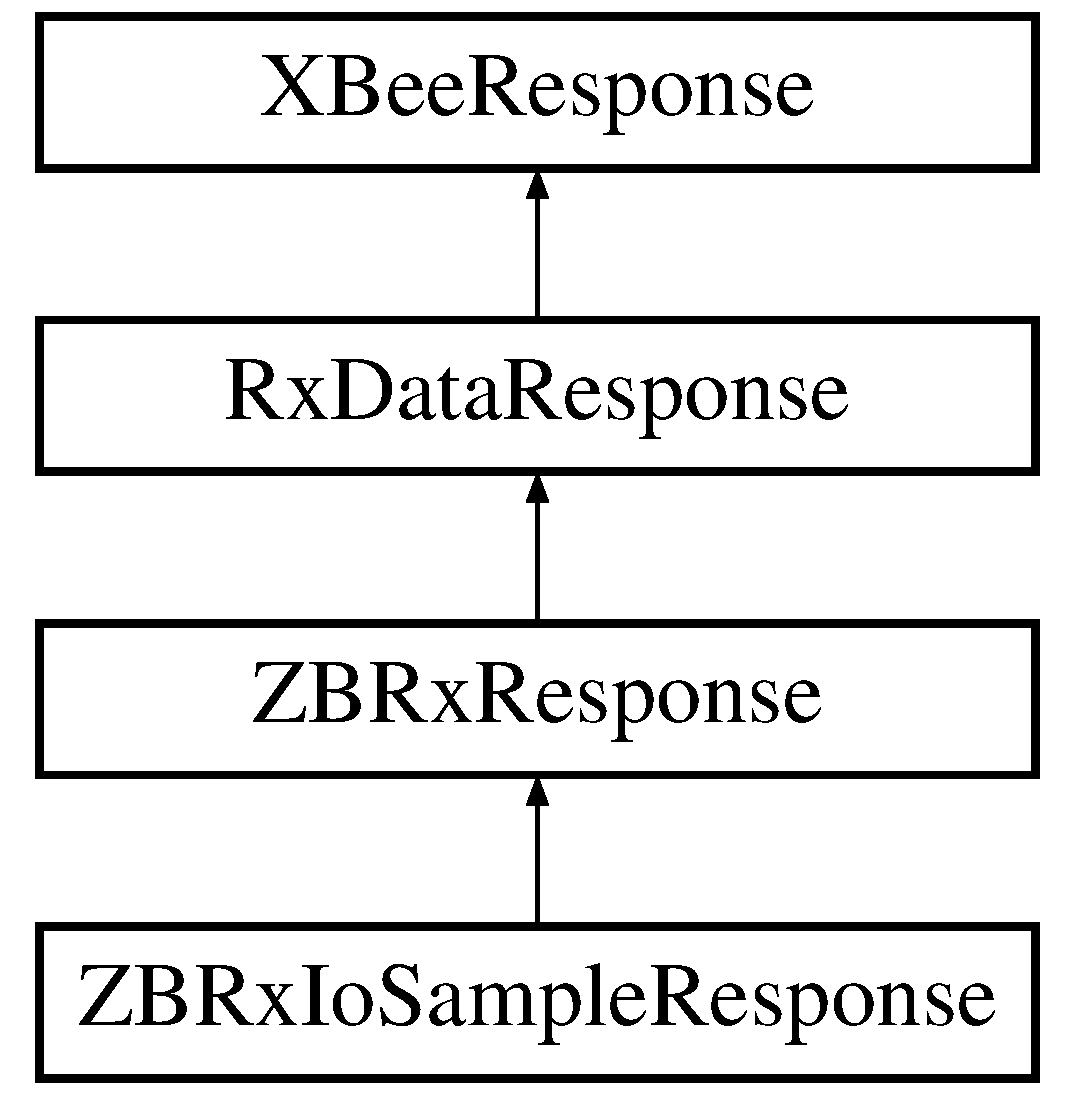
\includegraphics[height=4.000000cm]{classZBRxIoSampleResponse}
\end{center}
\end{figure}
\subsection*{\-Public \-Member \-Functions}
\begin{DoxyCompactItemize}
\item 
\hypertarget{classZBRxIoSampleResponse_ae1e501e3e940a1b199955d5c938e8970}{bool {\bfseries contains\-Analog} ()}\label{classZBRxIoSampleResponse_ae1e501e3e940a1b199955d5c938e8970}

\item 
\hypertarget{classZBRxIoSampleResponse_a12d70fd07c66e37ea06d8ae92672d320}{bool {\bfseries contains\-Digital} ()}\label{classZBRxIoSampleResponse_a12d70fd07c66e37ea06d8ae92672d320}

\item 
bool \hyperlink{classZBRxIoSampleResponse_ad0e444cc8854c996517c1ecde033a9c8}{is\-Analog\-Enabled} (uint8\-\_\-t pin)
\item 
bool \hyperlink{classZBRxIoSampleResponse_a946c653da11f62b319c3ca6606f8edff}{is\-Digital\-Enabled} (uint8\-\_\-t pin)
\item 
uint16\-\_\-t \hyperlink{classZBRxIoSampleResponse_aa74edf46988bd3e50ce4037350cbb91e}{get\-Analog} (uint8\-\_\-t pin)
\item 
bool \hyperlink{classZBRxIoSampleResponse_ac94f045360d7dbb009ac16bc437cbbd5}{is\-Digital\-On} (uint8\-\_\-t pin)
\item 
\hypertarget{classZBRxIoSampleResponse_af15dc5e0954ece81bb28b33316ad0fcd}{uint8\-\_\-t {\bfseries get\-Digital\-Mask\-Msb} ()}\label{classZBRxIoSampleResponse_af15dc5e0954ece81bb28b33316ad0fcd}

\item 
\hypertarget{classZBRxIoSampleResponse_a2bc101d5276c92f09ebe3a2f370ad0c2}{uint8\-\_\-t {\bfseries get\-Digital\-Mask\-Lsb} ()}\label{classZBRxIoSampleResponse_a2bc101d5276c92f09ebe3a2f370ad0c2}

\item 
\hypertarget{classZBRxIoSampleResponse_a065e15e00c505045a13e95091a62fae5}{uint8\-\_\-t {\bfseries get\-Analog\-Mask} ()}\label{classZBRxIoSampleResponse_a065e15e00c505045a13e95091a62fae5}

\end{DoxyCompactItemize}


\subsection{\-Detailed \-Description}
\-Represents a \-Series 2 \-R\-X \-I/\-O \-Sample packet 

\subsection{\-Member \-Function \-Documentation}
\hypertarget{classZBRxIoSampleResponse_aa74edf46988bd3e50ce4037350cbb91e}{\index{\-Z\-B\-Rx\-Io\-Sample\-Response@{\-Z\-B\-Rx\-Io\-Sample\-Response}!get\-Analog@{get\-Analog}}
\index{get\-Analog@{get\-Analog}!ZBRxIoSampleResponse@{\-Z\-B\-Rx\-Io\-Sample\-Response}}
\subsubsection[{get\-Analog}]{\setlength{\rightskip}{0pt plus 5cm}uint16\-\_\-t {\bf \-Z\-B\-Rx\-Io\-Sample\-Response\-::get\-Analog} (
\begin{DoxyParamCaption}
\item[{uint8\-\_\-t}]{pin}
\end{DoxyParamCaption}
)}}\label{classZBRxIoSampleResponse_aa74edf46988bd3e50ce4037350cbb91e}
\-Returns the 10-\/bit analog reading of the specified pin. \-Valid pins include \-A\-D\-C\-:xxx. \hypertarget{classZBRxIoSampleResponse_ad0e444cc8854c996517c1ecde033a9c8}{\index{\-Z\-B\-Rx\-Io\-Sample\-Response@{\-Z\-B\-Rx\-Io\-Sample\-Response}!is\-Analog\-Enabled@{is\-Analog\-Enabled}}
\index{is\-Analog\-Enabled@{is\-Analog\-Enabled}!ZBRxIoSampleResponse@{\-Z\-B\-Rx\-Io\-Sample\-Response}}
\subsubsection[{is\-Analog\-Enabled}]{\setlength{\rightskip}{0pt plus 5cm}bool {\bf \-Z\-B\-Rx\-Io\-Sample\-Response\-::is\-Analog\-Enabled} (
\begin{DoxyParamCaption}
\item[{uint8\-\_\-t}]{pin}
\end{DoxyParamCaption}
)}}\label{classZBRxIoSampleResponse_ad0e444cc8854c996517c1ecde033a9c8}
\-Returns true if the pin is enabled \hypertarget{classZBRxIoSampleResponse_a946c653da11f62b319c3ca6606f8edff}{\index{\-Z\-B\-Rx\-Io\-Sample\-Response@{\-Z\-B\-Rx\-Io\-Sample\-Response}!is\-Digital\-Enabled@{is\-Digital\-Enabled}}
\index{is\-Digital\-Enabled@{is\-Digital\-Enabled}!ZBRxIoSampleResponse@{\-Z\-B\-Rx\-Io\-Sample\-Response}}
\subsubsection[{is\-Digital\-Enabled}]{\setlength{\rightskip}{0pt plus 5cm}bool {\bf \-Z\-B\-Rx\-Io\-Sample\-Response\-::is\-Digital\-Enabled} (
\begin{DoxyParamCaption}
\item[{uint8\-\_\-t}]{pin}
\end{DoxyParamCaption}
)}}\label{classZBRxIoSampleResponse_a946c653da11f62b319c3ca6606f8edff}
\-Returns true if the pin is enabled \hypertarget{classZBRxIoSampleResponse_ac94f045360d7dbb009ac16bc437cbbd5}{\index{\-Z\-B\-Rx\-Io\-Sample\-Response@{\-Z\-B\-Rx\-Io\-Sample\-Response}!is\-Digital\-On@{is\-Digital\-On}}
\index{is\-Digital\-On@{is\-Digital\-On}!ZBRxIoSampleResponse@{\-Z\-B\-Rx\-Io\-Sample\-Response}}
\subsubsection[{is\-Digital\-On}]{\setlength{\rightskip}{0pt plus 5cm}bool {\bf \-Z\-B\-Rx\-Io\-Sample\-Response\-::is\-Digital\-On} (
\begin{DoxyParamCaption}
\item[{uint8\-\_\-t}]{pin}
\end{DoxyParamCaption}
)}}\label{classZBRxIoSampleResponse_ac94f045360d7dbb009ac16bc437cbbd5}
\-Returns true if the specified pin is high/on. \-Valid pins include \-D\-I\-O\-:xxx. 

\-The documentation for this class was generated from the following files\-:\begin{DoxyCompactItemize}
\item 
\-X\-Bee.\-h\item 
\-X\-Bee.\-cpp\end{DoxyCompactItemize}

\hypertarget{classZBRxResponse}{\section{\-Z\-B\-Rx\-Response \-Class \-Reference}
\label{classZBRxResponse}\index{\-Z\-B\-Rx\-Response@{\-Z\-B\-Rx\-Response}}
}


{\ttfamily \#include $<$\-X\-Bee.\-h$>$}

\-Inheritance diagram for \-Z\-B\-Rx\-Response\-:\begin{figure}[H]
\begin{center}
\leavevmode
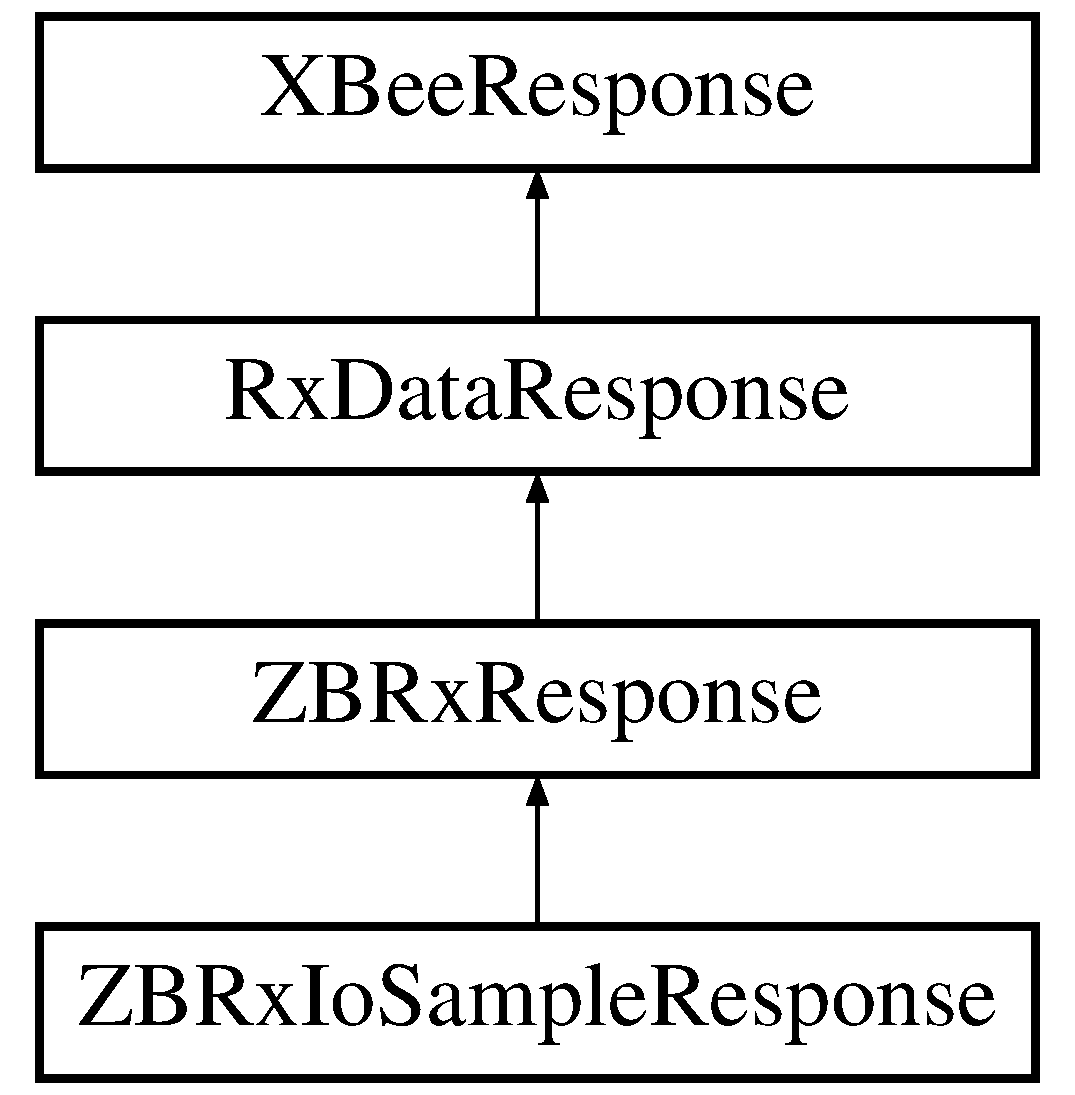
\includegraphics[height=4.000000cm]{classZBRxResponse}
\end{center}
\end{figure}
\subsection*{\-Public \-Member \-Functions}
\begin{DoxyCompactItemize}
\item 
\hypertarget{classZBRxResponse_a9af7b74ef6596f17312d7db042ba7e18}{\hyperlink{classXBeeAddress64}{\-X\-Bee\-Address64} \& {\bfseries get\-Remote\-Address64} ()}\label{classZBRxResponse_a9af7b74ef6596f17312d7db042ba7e18}

\item 
\hypertarget{classZBRxResponse_a5f7c9237a72e7f0107f2baf962ded78b}{uint16\-\_\-t {\bfseries get\-Remote\-Address16} ()}\label{classZBRxResponse_a5f7c9237a72e7f0107f2baf962ded78b}

\item 
\hypertarget{classZBRxResponse_a39ed277ac12274d7ae143a7cb27b219b}{uint8\-\_\-t {\bfseries get\-Option} ()}\label{classZBRxResponse_a39ed277ac12274d7ae143a7cb27b219b}

\item 
uint8\-\_\-t \hyperlink{classZBRxResponse_a9d2b73060d611bbdd581e0ceb195fd31}{get\-Data\-Length} ()
\item 
uint8\-\_\-t \hyperlink{classZBRxResponse_ad54e6ff3008f79d0ed32a78cc3d69151}{get\-Data\-Offset} ()
\end{DoxyCompactItemize}


\subsection{\-Detailed \-Description}
\-Represents a \-Series 2 \-R\-X packet 

\subsection{\-Member \-Function \-Documentation}
\hypertarget{classZBRxResponse_a9d2b73060d611bbdd581e0ceb195fd31}{\index{\-Z\-B\-Rx\-Response@{\-Z\-B\-Rx\-Response}!get\-Data\-Length@{get\-Data\-Length}}
\index{get\-Data\-Length@{get\-Data\-Length}!ZBRxResponse@{\-Z\-B\-Rx\-Response}}
\subsubsection[{get\-Data\-Length}]{\setlength{\rightskip}{0pt plus 5cm}uint8\-\_\-t {\bf \-Z\-B\-Rx\-Response\-::get\-Data\-Length} (
\begin{DoxyParamCaption}
{}
\end{DoxyParamCaption}
)\hspace{0.3cm}{\ttfamily  \mbox{[}virtual\mbox{]}}}}\label{classZBRxResponse_a9d2b73060d611bbdd581e0ceb195fd31}
\-Returns the length of the payload 

\-Implements \hyperlink{classRxDataResponse_a5845e6a0719fd0bf52675e47053a704e}{\-Rx\-Data\-Response}.

\hypertarget{classZBRxResponse_ad54e6ff3008f79d0ed32a78cc3d69151}{\index{\-Z\-B\-Rx\-Response@{\-Z\-B\-Rx\-Response}!get\-Data\-Offset@{get\-Data\-Offset}}
\index{get\-Data\-Offset@{get\-Data\-Offset}!ZBRxResponse@{\-Z\-B\-Rx\-Response}}
\subsubsection[{get\-Data\-Offset}]{\setlength{\rightskip}{0pt plus 5cm}uint8\-\_\-t {\bf \-Z\-B\-Rx\-Response\-::get\-Data\-Offset} (
\begin{DoxyParamCaption}
{}
\end{DoxyParamCaption}
)\hspace{0.3cm}{\ttfamily  \mbox{[}virtual\mbox{]}}}}\label{classZBRxResponse_ad54e6ff3008f79d0ed32a78cc3d69151}
\-Returns the position in the frame data where the data begins 

\-Implements \hyperlink{classRxDataResponse_a9e4b6bf4f1bfd9ccec45d190a204f61a}{\-Rx\-Data\-Response}.



\-The documentation for this class was generated from the following files\-:\begin{DoxyCompactItemize}
\item 
\-X\-Bee.\-h\item 
\-X\-Bee.\-cpp\end{DoxyCompactItemize}

\hypertarget{classZBTxRequest}{\section{\-Z\-B\-Tx\-Request \-Class \-Reference}
\label{classZBTxRequest}\index{\-Z\-B\-Tx\-Request@{\-Z\-B\-Tx\-Request}}
}


{\ttfamily \#include $<$\-X\-Bee.\-h$>$}

\-Inheritance diagram for \-Z\-B\-Tx\-Request\-:\begin{figure}[H]
\begin{center}
\leavevmode
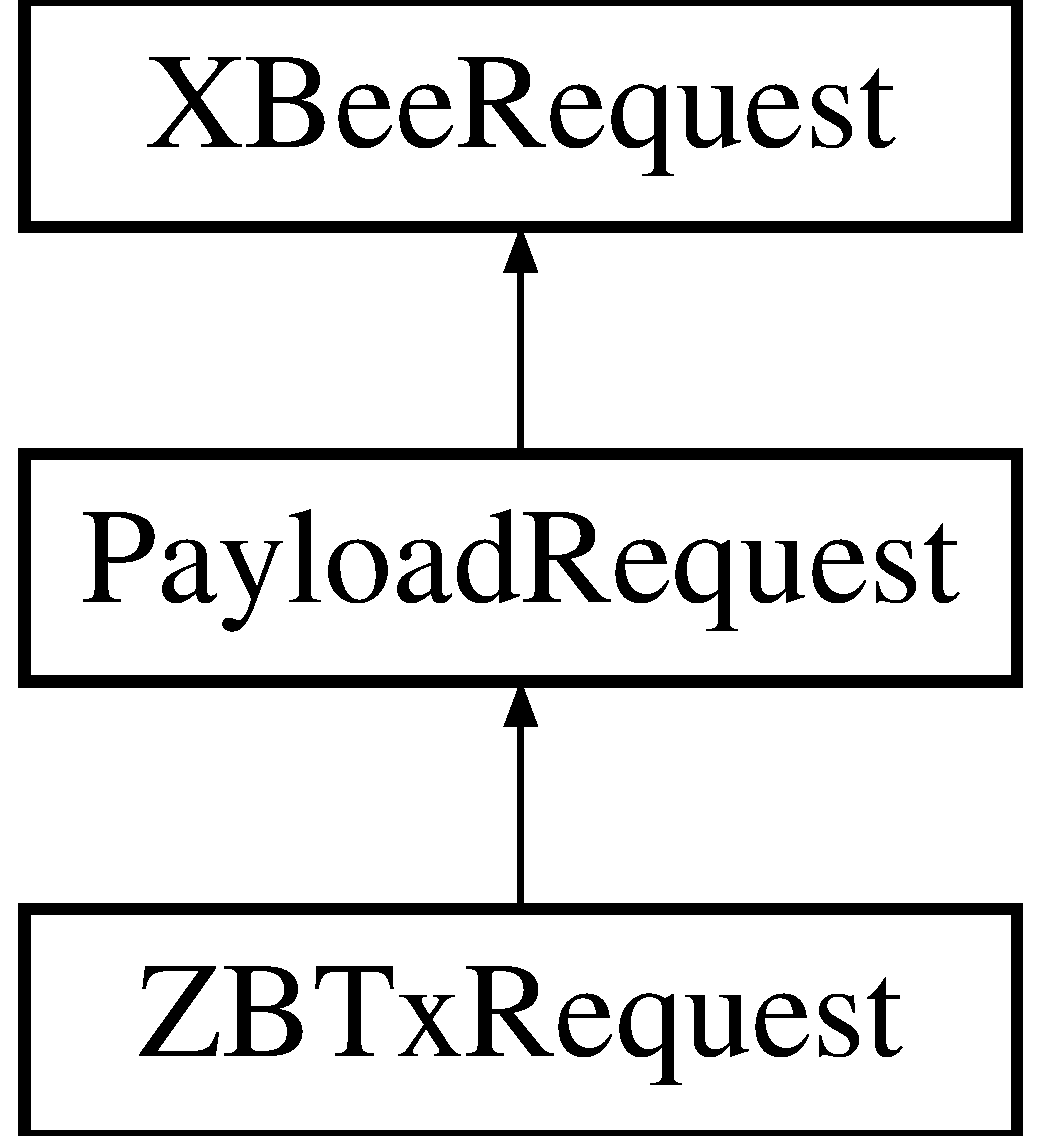
\includegraphics[height=3.000000cm]{classZBTxRequest}
\end{center}
\end{figure}
\subsection*{\-Public \-Member \-Functions}
\begin{DoxyCompactItemize}
\item 
\hyperlink{classZBTxRequest_a47d9d87e0ab2e155ff3408acea5dcf7c}{\-Z\-B\-Tx\-Request} (\hyperlink{classXBeeAddress64}{\-X\-Bee\-Address64} \&addr64, uint8\-\_\-t $\ast$payload, uint8\-\_\-t payload\-Length)
\item 
\hypertarget{classZBTxRequest_a98f109c346e669049697665745605e67}{{\bfseries \-Z\-B\-Tx\-Request} (\hyperlink{classXBeeAddress64}{\-X\-Bee\-Address64} \&addr64, uint16\-\_\-t addr16, uint8\-\_\-t broadcast\-Radius, uint8\-\_\-t option, uint8\-\_\-t $\ast$payload, uint8\-\_\-t payload\-Length, uint8\-\_\-t frame\-Id)}\label{classZBTxRequest_a98f109c346e669049697665745605e67}

\item 
\hyperlink{classZBTxRequest_a410499f31a049f0bd4bbc8299ec74e24}{\-Z\-B\-Tx\-Request} ()
\item 
\hypertarget{classZBTxRequest_adbd44bb9801c9cba0c9ea4e87ed8efa5}{\hyperlink{classXBeeAddress64}{\-X\-Bee\-Address64} \& {\bfseries get\-Address64} ()}\label{classZBTxRequest_adbd44bb9801c9cba0c9ea4e87ed8efa5}

\item 
\hypertarget{classZBTxRequest_ac75b0c6db3b6c9b54c3df2891b267950}{uint16\-\_\-t {\bfseries get\-Address16} ()}\label{classZBTxRequest_ac75b0c6db3b6c9b54c3df2891b267950}

\item 
\hypertarget{classZBTxRequest_a6c4a33cab93ff1d18703c8ddd4db4056}{uint8\-\_\-t {\bfseries get\-Broadcast\-Radius} ()}\label{classZBTxRequest_a6c4a33cab93ff1d18703c8ddd4db4056}

\item 
\hypertarget{classZBTxRequest_a4b97981c2a07afdeeacff09e479b7d45}{uint8\-\_\-t {\bfseries get\-Option} ()}\label{classZBTxRequest_a4b97981c2a07afdeeacff09e479b7d45}

\item 
\hypertarget{classZBTxRequest_a32725cca51a846b716308497d066b7a7}{void {\bfseries set\-Address64} (\hyperlink{classXBeeAddress64}{\-X\-Bee\-Address64} \&addr64)}\label{classZBTxRequest_a32725cca51a846b716308497d066b7a7}

\item 
\hypertarget{classZBTxRequest_aa1ae1761a27f335d353428de9c986aff}{void {\bfseries set\-Address16} (uint16\-\_\-t addr16)}\label{classZBTxRequest_aa1ae1761a27f335d353428de9c986aff}

\item 
\hypertarget{classZBTxRequest_a2d2825234b6d42385998df927d0fe0cb}{void {\bfseries set\-Broadcast\-Radius} (uint8\-\_\-t broadcast\-Radius)}\label{classZBTxRequest_a2d2825234b6d42385998df927d0fe0cb}

\item 
\hypertarget{classZBTxRequest_a32b2ea4b2c457396a7463e2add7e14f6}{void {\bfseries set\-Option} (uint8\-\_\-t option)}\label{classZBTxRequest_a32b2ea4b2c457396a7463e2add7e14f6}

\end{DoxyCompactItemize}
\subsection*{\-Protected \-Member \-Functions}
\begin{DoxyCompactItemize}
\item 
uint8\-\_\-t \hyperlink{classZBTxRequest_ac81e09dfbf7aefbdf7f8b4838b643c5c}{get\-Frame\-Data} (uint8\-\_\-t pos)
\item 
uint8\-\_\-t \hyperlink{classZBTxRequest_a8e6914c1f556981a0f863c57c57d053b}{get\-Frame\-Data\-Length} ()
\end{DoxyCompactItemize}


\subsection{\-Detailed \-Description}
\-Represents a \-Series 2 \-T\-X packet that corresponds to \-Api \-Id\-: \-Z\-B\-\_\-\-T\-X\-\_\-\-R\-E\-Q\-U\-E\-S\-T

\-Be careful not to send a data array larger than the max packet size of your radio. \-This class does not perform any validation of packet size and there will be no indication if the packet is too large, other than you will not get a \-T\-X \-Status response. \-The datasheet says 72 bytes is the maximum for \-Z\-Net firmware and \-Z\-B \-Pro firmware provides the \-A\-T\-N\-P command to get the max supported payload size. \-This command is useful since the maximum payload size varies according to certain settings, such as encryption. \-Z\-B \-Pro firmware provides a \-P\-A\-Y\-L\-O\-A\-D\-\_\-\-T\-O\-O\-\_\-\-L\-A\-R\-G\-E that is returned if payload size exceeds the maximum. 

\subsection{\-Constructor \& \-Destructor \-Documentation}
\hypertarget{classZBTxRequest_a47d9d87e0ab2e155ff3408acea5dcf7c}{\index{\-Z\-B\-Tx\-Request@{\-Z\-B\-Tx\-Request}!\-Z\-B\-Tx\-Request@{\-Z\-B\-Tx\-Request}}
\index{\-Z\-B\-Tx\-Request@{\-Z\-B\-Tx\-Request}!ZBTxRequest@{\-Z\-B\-Tx\-Request}}
\subsubsection[{\-Z\-B\-Tx\-Request}]{\setlength{\rightskip}{0pt plus 5cm}{\bf \-Z\-B\-Tx\-Request\-::\-Z\-B\-Tx\-Request} (
\begin{DoxyParamCaption}
\item[{{\bf \-X\-Bee\-Address64} \&}]{addr64, }
\item[{uint8\-\_\-t $\ast$}]{payload, }
\item[{uint8\-\_\-t}]{payload\-Length}
\end{DoxyParamCaption}
)}}\label{classZBTxRequest_a47d9d87e0ab2e155ff3408acea5dcf7c}
\-Creates a unicast \hyperlink{classZBTxRequest}{\-Z\-B\-Tx\-Request} with the \-A\-C\-K option and \-D\-E\-F\-A\-U\-L\-T\-\_\-\-F\-R\-A\-M\-E\-\_\-\-I\-D \hypertarget{classZBTxRequest_a410499f31a049f0bd4bbc8299ec74e24}{\index{\-Z\-B\-Tx\-Request@{\-Z\-B\-Tx\-Request}!\-Z\-B\-Tx\-Request@{\-Z\-B\-Tx\-Request}}
\index{\-Z\-B\-Tx\-Request@{\-Z\-B\-Tx\-Request}!ZBTxRequest@{\-Z\-B\-Tx\-Request}}
\subsubsection[{\-Z\-B\-Tx\-Request}]{\setlength{\rightskip}{0pt plus 5cm}{\bf \-Z\-B\-Tx\-Request\-::\-Z\-B\-Tx\-Request} (
\begin{DoxyParamCaption}
{}
\end{DoxyParamCaption}
)}}\label{classZBTxRequest_a410499f31a049f0bd4bbc8299ec74e24}
\-Creates a default instance of this class. \-At a minimum you must specify a payload, payload length and a destination address before sending this request. 

\subsection{\-Member \-Function \-Documentation}
\hypertarget{classZBTxRequest_ac81e09dfbf7aefbdf7f8b4838b643c5c}{\index{\-Z\-B\-Tx\-Request@{\-Z\-B\-Tx\-Request}!get\-Frame\-Data@{get\-Frame\-Data}}
\index{get\-Frame\-Data@{get\-Frame\-Data}!ZBTxRequest@{\-Z\-B\-Tx\-Request}}
\subsubsection[{get\-Frame\-Data}]{\setlength{\rightskip}{0pt plus 5cm}uint8\-\_\-t {\bf \-Z\-B\-Tx\-Request\-::get\-Frame\-Data} (
\begin{DoxyParamCaption}
\item[{uint8\-\_\-t}]{pos}
\end{DoxyParamCaption}
)\hspace{0.3cm}{\ttfamily  \mbox{[}protected, virtual\mbox{]}}}}\label{classZBTxRequest_ac81e09dfbf7aefbdf7f8b4838b643c5c}
\-Starting after the frame id (pos = 0) and up to but not including the checksum \-Note\-: \-Unlike \-Digi's definition of the frame data, this does not start with the \-A\-P\-I \-I\-D. \-The reason for this is the \-A\-P\-I \-I\-D and \-Frame \-I\-D are common to all requests, whereas my definition of frame data is only the \-A\-P\-I specific data. 

\-Implements \hyperlink{classXBeeRequest_ad5b998cd95a570bdaa4d74c6c8790d94}{\-X\-Bee\-Request}.

\hypertarget{classZBTxRequest_a8e6914c1f556981a0f863c57c57d053b}{\index{\-Z\-B\-Tx\-Request@{\-Z\-B\-Tx\-Request}!get\-Frame\-Data\-Length@{get\-Frame\-Data\-Length}}
\index{get\-Frame\-Data\-Length@{get\-Frame\-Data\-Length}!ZBTxRequest@{\-Z\-B\-Tx\-Request}}
\subsubsection[{get\-Frame\-Data\-Length}]{\setlength{\rightskip}{0pt plus 5cm}uint8\-\_\-t {\bf \-Z\-B\-Tx\-Request\-::get\-Frame\-Data\-Length} (
\begin{DoxyParamCaption}
{}
\end{DoxyParamCaption}
)\hspace{0.3cm}{\ttfamily  \mbox{[}protected, virtual\mbox{]}}}}\label{classZBTxRequest_a8e6914c1f556981a0f863c57c57d053b}
\-Returns the size of the api frame (not including frame id or api id or checksum). 

\-Implements \hyperlink{classXBeeRequest_a03b6c558db5836fa7167c0fba7405642}{\-X\-Bee\-Request}.



\-The documentation for this class was generated from the following files\-:\begin{DoxyCompactItemize}
\item 
\-X\-Bee.\-h\item 
\-X\-Bee.\-cpp\end{DoxyCompactItemize}

\hypertarget{classZBTxStatusResponse}{\section{\-Z\-B\-Tx\-Status\-Response \-Class \-Reference}
\label{classZBTxStatusResponse}\index{\-Z\-B\-Tx\-Status\-Response@{\-Z\-B\-Tx\-Status\-Response}}
}


{\ttfamily \#include $<$\-X\-Bee.\-h$>$}

\-Inheritance diagram for \-Z\-B\-Tx\-Status\-Response\-:\begin{figure}[H]
\begin{center}
\leavevmode
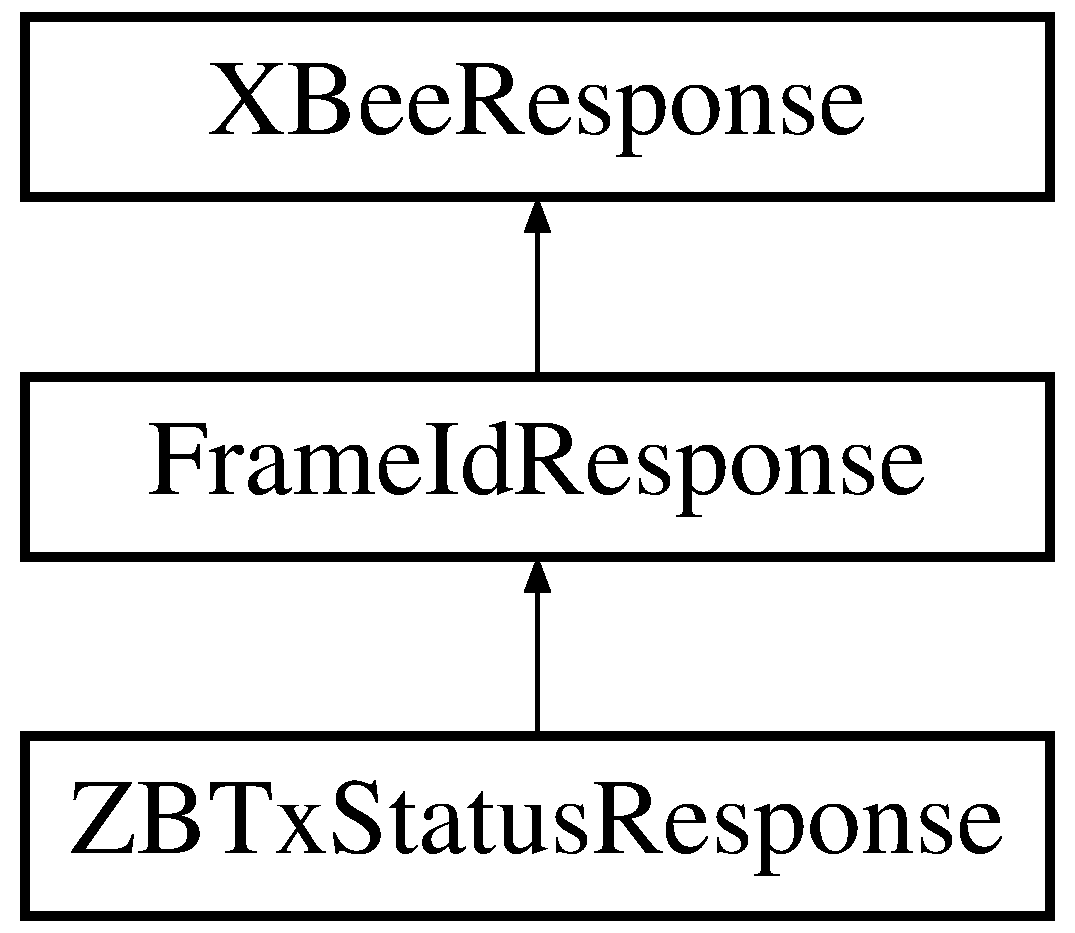
\includegraphics[height=3.000000cm]{classZBTxStatusResponse}
\end{center}
\end{figure}
\subsection*{\-Public \-Member \-Functions}
\begin{DoxyCompactItemize}
\item 
\hypertarget{classZBTxStatusResponse_a75043a3c9af5868938de65c2e4eb1196}{uint16\-\_\-t {\bfseries get\-Remote\-Address} ()}\label{classZBTxStatusResponse_a75043a3c9af5868938de65c2e4eb1196}

\item 
\hypertarget{classZBTxStatusResponse_a84f24560187b275d171f0abca28fe2a4}{uint8\-\_\-t {\bfseries get\-Tx\-Retry\-Count} ()}\label{classZBTxStatusResponse_a84f24560187b275d171f0abca28fe2a4}

\item 
\hypertarget{classZBTxStatusResponse_ad5b8d8a178e0f8fb69e7f24999c37a26}{uint8\-\_\-t {\bfseries get\-Delivery\-Status} ()}\label{classZBTxStatusResponse_ad5b8d8a178e0f8fb69e7f24999c37a26}

\item 
\hypertarget{classZBTxStatusResponse_a0a0a3e30c844a032b43e71f2cdcd66b8}{uint8\-\_\-t {\bfseries get\-Discovery\-Status} ()}\label{classZBTxStatusResponse_a0a0a3e30c844a032b43e71f2cdcd66b8}

\item 
\hypertarget{classZBTxStatusResponse_a3e8472bdc5c2a91a352c75ab327dcccc}{bool {\bfseries is\-Success} ()}\label{classZBTxStatusResponse_a3e8472bdc5c2a91a352c75ab327dcccc}

\end{DoxyCompactItemize}


\subsection{\-Detailed \-Description}
\-Represents a \-Series 2 \-T\-X status packet 

\-The documentation for this class was generated from the following files\-:\begin{DoxyCompactItemize}
\item 
\-X\-Bee.\-h\item 
\-X\-Bee.\-cpp\end{DoxyCompactItemize}

\printindex
\end{document}
